%-----------------------------------
% Define document and include general packages
%-----------------------------------
% Tabellen- und Abbildungsverzeichnis stehen normalerweise nicht im
% Inhaltsverzeichnis. Gleiches gilt für das Abkürzungsverzeichnis (siehe unten).
% Manche Dozenten bemängeln das. Die Optionen 'listof=totoc,bibliography=totoc'
% geben das Tabellen- und Abbildungsverzeichnis im Inhaltsverzeichnis (toc=Table
% of Content) aus.
% Da es aber verschiedene Regelungen je nach Dozent geben kann, werden hier
% beide Varianten dargestellt.
\documentclass[12pt,oneside,titlepage,listof=totoc,bibliography=totoc]{scrartcl}
%\documentclass[12pt,oneside,titlepage]{scrartcl}

%-----------------------------------
% Dokumentensprache
%-----------------------------------
%\def\FOMEN{}% Auskommentieren um die Dokumentensprache auf englisch zu ändern
\newif\ifde
\newif\ifen

%-----------------------------------
% Meta informationen
%-----------------------------------
%-----------------------------------
% Meta Informationen zur Arbeit
%-----------------------------------

% Autor
\newcommand{\myAutor}{Leopold Pinkernell}

% Adresse
\newcommand{\myAdresse}{Deipe Stegge 123 \\ \> \> \> 48653 Coesfeld}

% Titel der Arbeit
\newcommand{\myTitel}{Steuerung und Verwaltung von Servicerobotern}

% Untertitel der Arbeit
\newcommand{\myUntertitel}{Konzeption und prototypische Implementierung einer Webanwendung}

% Betreuer
\newcommand{\myBetreuer}{Prof. Dr. Jannik Hüls}

% Lehrveranstaltung
\newcommand{\myLehrveranstaltung}{Modul Nr. 1}

% Matrikelnummer
\newcommand{\myMatrikelNr}{564638}

% Ort
\newcommand{\myOrt}{Coesfeld}

% Datum der Abgabe
\newcommand{\myAbgabeDatum}{19. März 2024}

% Semesterzahl
\newcommand{\mySemesterZahl}{7}

% Name der Hochschule
\newcommand{\myHochschulName}{FOM Hochschule für Oekonomie \& Management}

% Standort der Hochschule
\newcommand{\myHochschulStandort}{Münster}

% Studiengang
\newcommand{\myStudiengang}{Wirtschaftsinformatik}

% Art der Arbeit
\newcommand{\myThesisArt}{Bachelor-Thesis}

% Zu erlangender akademische Grad
\newcommand{\myAkademischerGrad}{Bachelor of Science (B.Sc.)}

% Firma
\newcommand{\myFirma}{Tobit Software Laboratories AG}


\ifdefined\FOMEN
%Englisch
\entrue
\usepackage[english]{babel}
\else
%Deutsch
\detrue
\usepackage[ngerman]{babel}
\fi


\newcommand{\langde}[1]{%
   \ifde\selectlanguage{ngerman}#1\fi}
\newcommand{\langen}[1]{%
   \ifen\selectlanguage{english}#1\fi}
\usepackage[utf8]{luainputenc}
\langde{\usepackage[babel,german=quotes]{csquotes}}
\langen{\usepackage[babel,english=british]{csquotes}}
\usepackage[T1]{fontenc}
\usepackage{fancyhdr}
\usepackage{fancybox}
\usepackage[a4paper, left=4cm, right=2cm, top=4cm, bottom=2cm]{geometry}
\usepackage{graphicx}
\usepackage{colortbl}
\usepackage[capposition=top]{floatrow}
\usepackage{array}
\usepackage{float}      %Positionierung von Abb. und Tabellen mit [H] erzwingen
\usepackage{footnote}
% Darstellung der Beschriftung von Tabellen und Abbildungen (Leitfaden S. 44)
% singlelinecheck=false: macht die Caption linksbündig (statt zentriert)
% labelfont auf fett: (Tabelle x.y:, Abbildung: x.y)
% font auf fett: eigentliche Bezeichnung der Abbildung oder Tabelle
% Fettschrift laut Leitfaden 2018 S. 45
\usepackage[singlelinecheck=false, labelfont=bf, font=bf]{caption}
\usepackage{caption}
\usepackage{enumitem}
\usepackage{amssymb}
\usepackage{mathptmx}
%\usepackage{minted} %Kann für schöneres Syntax Highlighting genutzt werden. ACHTUNG: Python muss installiert sein.
\usepackage[scaled=0.9]{helvet} % Behebt, zusammen mit Package courier, pixelige Überschriften. Ist, zusammen mit mathptx, dem times-Package vorzuziehen. Details: https://latex-kurs.de/fragen/schriftarten/Times_New_Roman.html
\usepackage{courier}
\usepackage{amsmath}
\usepackage[table]{xcolor}
\usepackage{marvosym}			% Verwendung von Symbolen, z.B. perfektes Eurozeichen

\renewcommand\familydefault{\sfdefault}
\usepackage{ragged2e}

% Mehrere Fussnoten nacheinander mit Komma separiert
\usepackage[hang,multiple]{footmisc}
\setlength{\footnotemargin}{1em}

% todo Aufgaben als Kommentare verfassen für verschiedene Editoren
\usepackage{todonotes}

% Verhindert, dass nur eine Zeile auf der nächsten Seite steht
\setlength{\marginparwidth}{2cm}
\usepackage[all]{nowidow}

%-----------------------------------
% Farbdefinitionen
%-----------------------------------
\definecolor{darkblack}{rgb}{0,0,0}
\definecolor{dunkelgrau}{rgb}{0.8,0.8,0.8}
\definecolor{hellgrau}{rgb}{0.0,0.7,0.99}
\definecolor{mauve}{rgb}{0.58,0,0.82}
\definecolor{dkgreen}{rgb}{0,0.6,0}

%-----------------------------------
% Pakete für Tabellen
%-----------------------------------
\usepackage{epstopdf}
\usepackage{nicefrac} % Brüche
\usepackage{multirow}
\usepackage{rotating} % vertikal schreiben
\usepackage{mdwlist}
\usepackage{tabularx}% für Breitenangabe

%-----------------------------------
% sauber formatierter Quelltext
%-----------------------------------
\usepackage{listings}
% JavaScript als Sprache definieren:
\lstdefinelanguage{JavaScript}{
	keywords={break, super, case, extends, switch, catch, finally, for, const, function, try, continue, if, typeof, debugger, var, default, in, void, delete, instanceof, while, do, new, with, else, return, yield, enum, let, await},
	keywordstyle=\color{blue}\bfseries,
	ndkeywords={class, export, boolean, throw, implements, import, this, interface, package, private, protected, public, static},
	ndkeywordstyle=\color{darkgray}\bfseries,
	identifierstyle=\color{black},
	sensitive=false,
	comment=[l]{//},
	morecomment=[s]{/*}{*/},
	commentstyle=\color{purple}\ttfamily,
	stringstyle=\color{red}\ttfamily,
	morestring=[b]',
	morestring=[b]"
}

\lstset{
	%language=JavaScript,
	numbers=left,
	numberstyle=\tiny,
	numbersep=5pt,
	breaklines=true,
	showstringspaces=false,
	frame=l ,
	xleftmargin=5pt,
	xrightmargin=5pt,
	basicstyle=\ttfamily\scriptsize,
	stepnumber=1,
	keywordstyle=\color{blue},          % keyword style
  	commentstyle=\color{dkgreen},       % comment style
  	stringstyle=\color{mauve}         % string literal style
}

%-----------------------------------
%Literaturverzeichnis Einstellungen
%-----------------------------------

% Biblatex

\usepackage{url}
\urlstyle{same}

\usepackage[
backend=biber,
style=ieee,
maxcitenames=3,	% mindestens 3 Namen ausgeben bevor et. al. kommt
maxbibnames=999,
date=iso,
seconds=true, %werden nicht verwendet, so werden aber Warnungen unterdrückt.
urldate=iso,
dashed=false,
autocite=inline,
useprefix=true, % 'von' im Namen beachten (beim Anzeigen)
mincrossrefs = 1
]{biblatex}%iso dateformat für YYYY-MM-DD

%% et al. anstatt u. a. bei mehr als drei Autoren.
\DefineBibliographyStrings{ngerman}{ 
	andothers = {{et\,al\adddot}},             
}
\DefineBibliographyStrings{english}{ 
	andothers = {{et\,al\adddot}},             
}

%weitere Anpassungen für BibLaTex
% Opptionen für Biblatex
\ExecuteBibliographyOptions{%
giveninits=false,
isbn=true,
url=true,
doi=false,
eprint=false,
maxbibnames=7, % Alle Autoren (kein et al.)
maxcitenames=3, % et al. ab dem 3. Autor
backref=false, % Rückverweise auf Zitatseiten
bibencoding=utf8, % wenn .bib in utf8, sonst ascii
bibwarn=true, % Warnung bei fehlerhafter bib-Datei
}%

% et al. an Stelle von u.a.
\DefineBibliographyStrings{ngerman}{
   andothers = {{et\,al\adddot}},
}

% Klammern um das Jahr in der Fußnote
\renewbibmacro*{cite:labelyear+extrayear}{%
  \iffieldundef{labelyear}
    {}
    {\printtext[bibhyperref]{%
       \mkbibparens{%
         \printfield{labelyear}%
         \printfield{extrayear}}}}}

\renewbibmacro*{cite:title}{%
  \printtext[bibhyperref]{%
    \printfield[citetitle]{labeltitle}%
    \setunit{\addcomma\space}%
    \printdate}}

\DeclareNameFormat{last-first}{%
  \iffirstinits
    {\usebibmacro{name:family-given}
        {\namepartfamily}
        {\namepartgiveni}
        {\namepartprefix}
        {\namepartsuffix}
    }
    {\usebibmacro{name:family-given}
        {\namepartfamily}
        {\namepartgiven}
        {\namepartprefix}
        {\namepartsuffix}
    }%
  \usebibmacro{name:andothers}}

% Alternative Notation der Fußnoten
% Zeigt sowohl den Nachnamen als auch den Vornamen an
% Beispiel: \fullfootcite[Vgl. ][Seite 5]{Tanenbaum.2003}
\DeclareCiteCommand{\fullfootcite}[\mkbibfootnote]
  {\usebibmacro{prenote}}
  {\usebibmacro{citeindex}%
    \printnames[sortname][1-1]{author}%
    \addspace (\printfield{year})}
  {\addsemicolon\space}
  {\usebibmacro{postnote}}

%Autoren (Nachname, Vorname)
\DeclareNameAlias{default}{family-given}

%Reihenfolge von publisher, year, address verändern
% Achtung, bisher nur für den Typ @book definiert

%% Definiert @Book Eintrag
\DeclareBibliographyDriver{book}{%
  \printnames{author}%
  \newunit\addcolon\space
  \printfield{title}%
  \setunit*{,\space}%
  \printfield{edition}%
  \setunit*{\addcomma\space}%
  \printlist{publisher}%
  \newunit\newblockpunct
  \printlist{location}%
  \setunit*{\space}%
  \printfield{year}%
  \setunit*{,\space}%
  \printfield{isbn}%
  \finentry}

%% Definiert @Online Eintrag
\DeclareBibliographyDriver{online}{%
  \printnames{author}%
  \newunit\addcolon\space
  \printfield{title}%
  \setunit*{,\space}%
  %\newunit\newblock
  \printfield{url}%
  \setunit{,\space Erscheinungsjahr:\space}%
  \printfield{year}%
  \setunit{,\space Zugriff am:\space}%
  \printfield{note}%
  \finentry}

%% Definiert @Software Eintrag
\DeclareBibliographyDriver{software}{%
  \printnames{author}%
  \newunit\addcolon\space
  \printfield{title}%
  \setunit*{,\space}%
  %\newunit\newblock
  \setunit*{,\space Verfügbar unter:\space}%
  \printfield[noformat]{url}%
  \setunit*{,\space Version:\space}%
  \printfield[noformat]{version}%
  \setunit*{,\space Zugriff am:\space}%
  \printfield{note}%
  \finentry}

%% Definiert @Article Eintrag
\DeclareBibliographyDriver{article}{%
  \printnames{author}%
  \newunit\newblockpunct
  \printfield{title}%
  \setunit*{.\space In:\space}%
  %\newunit\newblock
  \usebibmacro{journal}%
  \setunit*{\space (}%
  \printfield{year}\newunit{)}%
  \finentry}

%% Definiert @InProceedings Eintrag
\DeclareBibliographyDriver{inproceedings}{%
	\printnames{author}%
	\setunit*{,\space (}%
	\printfield{year}\newunit{)}%
	\newunit\newblockpunct
	\printfield{title}%
	\setunit*{\space}%
	\usebibmacro{booktitle}%
	\setunit*{,\space}%
	\printfield{isbn}%
	\setunit*{,\space}%
	\printfield{doi}%
	\finentry}

%Doppelpunkt nach dem letzten Autor
\renewcommand*{\labelnamepunct}{\addcolon\addspace }

%Komma an Stelle des Punktes
\renewcommand*{\newunitpunct}{\addcomma\space}

%Autoren durch Semikolon trennen
\newcommand*{\bibmultinamedelim}{\addsemicolon\space}%
\newcommand*{\bibfinalnamedelim}{\addsemicolon\space}%
\AtBeginBibliography{%
  \let\multinamedelim\bibmultinamedelim
  \let\finalnamedelim\bibfinalnamedelim
}

%Titel nicht kursiv anzeigen
\DeclareFieldFormat{title}{#1\isdot}


%%%% Ende Alter Leitfaden

%Bib-Datei einbinden
\addbibresource{literatur/literatur.bib}
\addbibresource{literatur/internet.bib}
\addbibresource{literatur/software.bib}

% Zeilenabstand im Literaturverzeichnis ist Einzeilig
% siehe Leitfaden S. 14
\AtBeginBibliography{\singlespacing}

%-----------------------------------
% Silbentrennung
%-----------------------------------
\usepackage{hyphsubst}
\HyphSubstIfExists{ngerman-x-latest}{%
\HyphSubstLet{ngerman}{ngerman-x-latest}}{}

%-----------------------------------
% Pfad fuer Abbildungen
%-----------------------------------
\graphicspath{{./}{./abbildungen/}}

%-----------------------------------
% Weitere Ebene einfügen
%-----------------------------------
\usepackage{titletoc}

\makeatletter

% Setze die Tiefe des Inhaltsverzeichnis auf 4 Ebenen
% Damit erscheinen \paragraph-Sektionen auch im Inhaltsverzeichnis
\setcounter{secnumdepth}{4}
\setcounter{tocdepth}{4}

% Fuege Abstand nach unten wie in einer normalen \section hinzu
% Andernfalls haette \paragraph keinen Zeilenumbruch
% Der Zeilenumbruch koennte mit einer leeren \mbox{} ersetzt werden
% Jedoch klebt dann der Text relativ nah an der Ueberschrift
\renewcommand{\paragraph}{%
  \@startsection{paragraph}{4}%
  {\z@}{3.25ex \@plus 1ex \@minus .2ex}{1.5ex plus 0.2ex}%
  {\normalfont\normalsize\bfseries\sffamily}%
}

\makeatother


%-----------------------------------
% Paket für die Nutzung von Anhängen
%-----------------------------------
\usepackage{appendix}

%-----------------------------------
% Zeilenabstand 1,5-zeilig
%-----------------------------------
\usepackage{setspace}
\onehalfspacing

%-----------------------------------
% Absätze durch eine neue Zeile
%-----------------------------------
\setlength{\parindent}{0mm}
\setlength{\parskip}{0.8em plus 0.5em minus 0.3em}

\sloppy					%Abstände variieren
\pagestyle{headings}

%----------------------------------
% Präfix in das Abbildungs- und Tabellenverzeichnis aufnehmen, statt nur der Nummerierung (siehe Issue #206).
%----------------------------------
\KOMAoption{listof}{entryprefix} % Siehe KOMA-Script Doku v3.28 S.153
\BeforeStartingTOC[lof]{\renewcommand*\autodot{:}} % Für den Doppelpunkt hinter Präfix im Abbildungsverzeichnis
\BeforeStartingTOC[lot]{\renewcommand*\autodot{:}} % Für den Doppelpunkt hinter Präfix im Tabellenverzeichnis

%-----------------------------------
% Abkürzungsverzeichnis
%-----------------------------------
\usepackage[printonlyused]{acronym}

%-----------------------------------
% Symbolverzeichnis
%-----------------------------------
% Quelle: https://www.namsu.de/Extra/pakete/Listofsymbols.pdf
\usepackage[final]{listofsymbols}

%-----------------------------------
% Glossar
%-----------------------------------
\usepackage{glossaries}
\glstoctrue %Auskommentieren, damit das Glossar nicht im Inhaltsverzeichnis angezeigt wird.
\makenoidxglossaries
\newglossaryentry{HTTP}{name={HTTP},description={Das Hypertext Transfer Protocol ist ein grundlegendes Protokoll für den Datenaustausch im World Wide Web, das die Übertragung von Hypertext-Dokumenten zwischen Webbrowsern und -servern ermöglicht und durch Zustandslosigkeit, verschiedene Methoden (GET, POST), Statuscodes und die Verwendung von URLs gekennzeichnet ist}}
\newglossaryentry{MQTT}{name={MQTT},description={Message Queuing Telemetry Transport ist ein leichtgewichtiges Netzwerkprotokoll für die effiziente Nachrichtenübertragung zwischen Geräten, besonders in Machine-to-Machine (M2M) und Internet of Things (IoT)-Anwendungen}}
\newglossaryentry{Webhook}{name={Webhook},description={Ein Webhook ist eine automatisierte Methode zur Übertragung von Echtzeitinformationen zwischen Webdiensten durch das Senden von HTTP-POST-Anfragen an vordefinierte URLs, um sofortige Ereignisbenachrichtigungen zu ermöglichen}}
\newglossaryentry{Websocket}{name={Websocket}, description={Ein Kommunikationsprotokoll, das eine bidirektionale, echtzeitfähige Verbindung zwischen einem Webbrowser und einem Server ermöglicht, wodurch eine kontinuierliche Datenübertragung für interaktive Webanwendungen in Echtzeit ermöglicht wird}}
\newglossaryentry{Mockup}{name={Mockup}, description={Eine visuelle Darstellung oder Modellierung eines Designs, Produkts oder einer Benutzeroberfläche, die dazu dient, das Aussehen und die Funktionalität zu skizzieren und Feedback zu sammeln, bevor die eigentliche Entwicklung beginnt}}
\newglossaryentry{Base64}{name={Base64}, description={Base64 ist ein Kodierungsverfahren, das Binärdaten in eine Textdarstellung umwandelt, indem 64 verschiedene ASCII-Zeichen verwendet werden, wodurch die Daten für die Übertragung über textbasierte Protokolle geeignet gemacht werden}}
\newglossaryentry{DOM}{name={DOM}, description={Das Document Object Model ist eine Programmierschnittstelle, die die Struktur und Inhalte eines HTML- oder XML-Dokuments repräsentiert und es ermöglicht, auf diese Elemente zuzugreifen, sie zu ändern und zu manipulieren}}
\newglossaryentry{Mixins}{name={Mixins}, description={Sass Mixins sind wiederverwendbare Code-Ausschnitte in Sass, die dazu dienen, CSS-Eigenschaften und -Werte zu kapseln und sie leicht in verschiedenen Stilen oder Elementen anzuwenden}}

%-----------------------------------
% PDF Meta Daten setzen
%-----------------------------------
\usepackage[hyperfootnotes=false]{hyperref} %hyperfootnotes=false deaktiviert die Verlinkung der Fußnote. Ansonsten inkompaibel zum Paket "footmisc"
% Behebt die falsche Darstellung der Lesezeichen in PDF-Dateien, welche eine Übersetzung besitzen
% siehe Issue 149
\makeatletter
\pdfstringdefDisableCommands{\let\selectlanguage\@gobble}
\makeatother

\hypersetup{
    pdfinfo={
        Title={\myTitel} - {\myUntertitel},
        Subject={\myStudiengang},
        Author={\myAutor},
        Build=1.1
    }
}

%-----------------------------------
% PlantUML
%-----------------------------------
%\usepackage{plantuml}

%-----------------------------------
% Umlaute in Code korrekt darstellen
% siehe auch: https://en.wikibooks.org/wiki/LaTeX/Source_Code_Listings
%-----------------------------------
\lstset{literate=
	{á}{{\'a}}1 {é}{{\'e}}1 {í}{{\'i}}1 {ó}{{\'o}}1 {ú}{{\'u}}1
	{Á}{{\'A}}1 {É}{{\'E}}1 {Í}{{\'I}}1 {Ó}{{\'O}}1 {Ú}{{\'U}}1
	{à}{{\`a}}1 {è}{{\`e}}1 {ì}{{\`i}}1 {ò}{{\`o}}1 {ù}{{\`u}}1
	{À}{{\`A}}1 {È}{{\'E}}1 {Ì}{{\`I}}1 {Ò}{{\`O}}1 {Ù}{{\`U}}1
	{ä}{{\"a}}1 {ë}{{\"e}}1 {ï}{{\"i}}1 {ö}{{\"o}}1 {ü}{{\"u}}1
	{Ä}{{\"A}}1 {Ë}{{\"E}}1 {Ï}{{\"I}}1 {Ö}{{\"O}}1 {Ü}{{\"U}}1
	{â}{{\^a}}1 {ê}{{\^e}}1 {î}{{\^i}}1 {ô}{{\^o}}1 {û}{{\^u}}1
	{Â}{{\^A}}1 {Ê}{{\^E}}1 {Î}{{\^I}}1 {Ô}{{\^O}}1 {Û}{{\^U}}1
	{œ}{{\oe}}1 {Œ}{{\OE}}1 {æ}{{\ae}}1 {Æ}{{\AE}}1 {ß}{{\ss}}1
	{ű}{{\H{u}}}1 {Ű}{{\H{U}}}1 {ő}{{\H{o}}}1 {Ő}{{\H{O}}}1
	{ç}{{\c c}}1 {Ç}{{\c C}}1 {ø}{{\o}}1 {å}{{\r a}}1 {Å}{{\r A}}1
	{€}{{\EUR}}1 {£}{{\pounds}}1 {„}{{\glqq{}}}1
}

%-----------------------------------
% Kopfbereich / Header definieren
%-----------------------------------
\pagestyle{fancy}
\fancyhf{}
% Seitenzahl oben, mittig, mit Strichen beidseits
% \fancyhead[C]{-\ \thepage\ -}

% Seitenzahl oben, mittig, entsprechend Leitfaden ohne Striche beidseits
\fancyhead[C]{\thepage}
%\fancyhead[L]{\leftmark}							% kein Footer vorhanden
% Waagerechte Linie unterhalb des Kopfbereiches anzeigen. Laut Leitfaden ist
% diese Linie nicht erforderlich. Ihre Breite kann daher auf 0pt gesetzt werden.
\renewcommand{\headrulewidth}{0.4pt}
%\renewcommand{\headrulewidth}{0pt}

%-----------------------------------
% Damit die hochgestellten Zahlen auch auf die Fußnote verlinkt sind (siehe Issue 169)
%-----------------------------------
\hypersetup{colorlinks=true, breaklinks=true, linkcolor=darkblack, citecolor=darkblack, menucolor=darkblack, urlcolor=darkblack, linktoc=all, bookmarksnumbered=false, pdfpagemode=UseOutlines, pdftoolbar=true}
\urlstyle{same}%gleiche Schriftart für den Link wie für den Text

%-----------------------------------
% Start the document here:
%-----------------------------------
\begin{document}

\pagenumbering{Roman}								% Seitennumerierung auf römisch umstellen
\newcolumntype{C}{>{\centering\arraybackslash}X}	% Neuer Tabellen-Spalten-Typ:
%Zentriert und umbrechbar

%-----------------------------------
% Textcommands
%-----------------------------------
%----------------------------------
%  TextCommands
%----------------------------------
%
%
%
%
%----------------------------------
%  common textCommands
%----------------------------------
% Information: OL bedeutet ohne Leerzeichen. Damit man dieses Command z. B. vor einem Komma oder vor einem anderen Zeichen verwenden kann. Dies ist ein Best-Practis von mir und hat sich sehr bewehrt.
% Allgemein hat es sich bewert alle Wörter die man häufig schreibt und wahrscheinlich falsch oder unterscheidlich schreibt, als Textcommand zu hinterlegen.
% 
%
%
\renewcommand{\symheadingname}{\langde{Symbolverzeichnis}\langen{List of Symbols}}
\newcommand{\abbreHeadingName}{\langde{Abkürzungsverzeichnis}\langen{List of Abbreviations}}
\newcommand{\headingNameInternetSources}{\langde{Internetquellen}\langen{Internet sources}}
\newcommand{\AppendixName}{\langde{Anhang}\langen{Appendix}}
\newcommand{\vglf}{\langde{Vgl.}\langen{compare}}
\newcommand{\pagef}{\langde{S. }\langen{p. }}
\newcommand{\os}{\mbox{o. S}}
\newcommand{\ojol}{\mbox{o. J.}}
\newcommand{\oj}{\ojol\ }
\newcommand{\og}{\mbox{o. g.}\ }
\newcommand{\ua}{\mbox{u. a.}\ }
\newcommand{\dah}{\mbox{d. h.}\ }
\newcommand{\zbol}{\mbox{z. B.}}
\newcommand{\zb}{\zbol\ }
\newcommand{\uamol}{unter anderem}
\newcommand{\uam}{\uamol\ }
\newcommand{\uanol}{unter anderen}%mit Leerzeichen
\newcommand{\uan}{\uanol\ }%mit Leerzeichen
\newcommand{\abbol}{Ab"-bil"-dung}
\newcommand{\abb}{\abbol\ }
\newcommand{\tabol}{Tabelle}
\newcommand{\tab}{\tabol\ }
\newcommand{\ggfol}{ggf.}
\newcommand{\ggf}{\ggfol\ }
\newcommand{\unodol}{und/oder}
\newcommand{\unod}{\unodol\ }
\newcommand{\deckgl}{deck.gl}
\newcommand{\loadersgl}{loaders.gl}
\newcommand{\obj}{.obj}
\newcommand{\mtl}{.mtl}
\newcommand{\gltf}{.gltf}
\newcommand{\glb}{.glb}

%----------------------------------
% project individual textCommands
%----------------------------------
\newcommand{\lehol}{Lebensmitteleinzelhandel}%Beispiel eines langen Wortes
\newcommand{\leh}{\lehol\ }

\newcommand{\green}{\cellcolor{green!25}}
\newcommand{\yellow}{\cellcolor{yellow!25}}
\newcommand{\red}{\cellcolor{red!25}}

%-----------------------------------
% Titlepage
%-----------------------------------
\begin{titlepage}
	\newgeometry{left=2cm, right=2cm, top=2cm, bottom=2cm}
	\begin{center}
    
\includegraphics[width=2.3cm]{abbildungen/fomLogo} \\
    \vspace{.5cm}
		\begin{Large}\textbf{\myHochschulName}\end{Large}\\
    \vspace{.5cm}
		\begin{Large}Hochschulzentrum \myHochschulStandort\end{Large}\\
		\vspace{2cm}
    \begin{Large}\textbf{\myThesisArt}\end{Large}\\
    \vspace{.5cm}
    im Studiengang \myStudiengang
		\vspace{1.7cm}

		zur Erlangung des Grades eines\\
    \vspace{0.5cm}
		\begin{Large}{\myAkademischerGrad}\end{Large}\\
		\vspace{1.8cm}
		über das Thema\\
    \vspace{0.5cm}
		\large{\textbf{\myTitel}}\\
		{\myUntertitel}\\
		\vspace{2cm}
    von\\
    \vspace{0.5cm}
    \begin{Large}{\myAutor}\end{Large}\\
	\end{center}
	\normalsize
	\vfill
    \begin{tabular}{ l l }
        Erstgutachter: & \myBetreuer\\
        Matrikelnummer: & \myMatrikelNr\\
        Abgabedatum: & \myAbgabeDatum\\
    \end{tabular}
\end{titlepage}


%-----------------------------------
% Vorwort (optional; bei Verwendung beide Zeilen entkommentieren und unter Inhaltsverzeichnis setcounter entsprechend anpassen)
%-----------------------------------
%\section*{Vorwort}
Bei Bedarf erscheint vor dem Inhaltsverzeichnis ein Vorwort. Es erhält keine Kapitelnummer und wird nicht im Inhaltsverzeichnis aufgeführt (Auszug aus dem Leitfaden zur Gestaltung wissenschaftlicher Arbeiten / Dekanat ING \& IT Management, Februar 2022).

Lorem ipsum dolor sit amet, consetetur sadipscing elitr, sed diam nonumy eirmod tempor invidunt ut labore et dolore magna aliquyam erat, sed diam voluptua. At vero eos et accusam et justo duo dolores et ea rebum. Stet clita kasd gubergren, no sea takimata sanctus est Lorem ipsum dolor sit amet. Lorem ipsum dolor sit amet, consetetur sadipscing elitr, sed diam nonumy eirmod tempor invidunt ut labore et dolore magna aliquyam erat, sed diam voluptua. At vero eos et accusam et justo duo dolores et ea rebum. Stet clita kasd gubergren, no sea takimata sanctus est Lorem ipsum dolor sit amet. Lorem ipsum dolor sit amet, consetetur sadipscing elitr, sed diam nonumy eirmod tempor invidunt ut labore et dolore magna aliquyam erat, sed diam voluptua. At vero eos et accusam et justo duo dolores et ea rebum. Stet clita kasd gubergren, no sea takimata sanctus est Lorem ipsum dolor sit amet. 

Duis autem vel eum iriure dolor in hendrerit in vulputate velit esse molestie consequat, vel illum dolore eu feugiat nulla facilisis at vero eros et accumsan et iusto odio dignissim qui blandit praesent luptatum zzril delenit augue duis dolore te feugait nulla facilisi. Lorem ipsum dolor sit amet, consectetuer adipiscing elit, sed diam nonummy nibh euismod tincidunt ut laoreet dolore magna aliquam erat volutpat. 
\\[1cm]
{\myOrt}, März 2022

{\myAutor}
%\newpage

%-----------------------------------
% Inhaltsverzeichnis
%-----------------------------------
% Um das Tabellen- und Abbbildungsverzeichnis zu de/aktivieren ganz oben in Documentclass schauen
\setcounter{page}{2}
\addtocontents{toc}{\protect\enlargethispage{-20mm}}% Die Zeile sorgt dafür, dass das Inhaltsverzeichnisseite auf die zweite Seite gestreckt wird und somit schick aussieht. Das sollte eigentlich automatisch funktionieren. Wer rausfindet wie, kann das gern ändern.
\setcounter{tocdepth}{4}
\tableofcontents
\newpage

%-----------------------------------
% Abbildungsverzeichnis
%-----------------------------------
\listoffigures
\newpage
%-----------------------------------
% Tabellenverzeichnis
%-----------------------------------
\listoftables
\newpage
%-----------------------------------
% Abkürzungsverzeichnis
%-----------------------------------
% Falls das Abkürzungsverzeichnis nicht im Inhaltsverzeichnis angezeigt werden soll
% dann folgende Zeile auskommentieren.
\addcontentsline{toc}{section}{\abbreHeadingName}

\section*{\langde{Abkürzungsverzeichnis}\langen{List of Abbreviations}}
% TODO Set longest acronym!
\begin{acronym}[WYSIWYG]\itemsep0pt %der Parameter in Klammern sollte die längste Abkürzung sein. Damit wird der Abstand zwischen Abkürzung und Übersetzung festgelegt
  \acro{IFR}{International Federation of Robotics}
  \acro{DSR}{Design Science Research}
  \acro{BA}{Bundesagentur für Arbeit}
  \acro{BCB}{Bot Control Backend}
\end{acronym}
\newpage

%-----------------------------------
% Symbolverzeichnis
%-----------------------------------
% In Overleaf führt der Einsatz des Symbolverzeichnisses zu einem Fehler, der aber ignoriert werdne kann
% Falls das Symbolverzeichnis nicht im Inhaltsverzeichnis angezeigt werden soll
% dann folgende Zeile auskommentieren.
%\phantomsection\addcontentsline{toc}{section}{\symheadingname}
%%
%
%
%
%
%
%
% Quelle: https://www.namsu.de/Extra/pakete/Listofsymbols.pdf
% Wie ind er Quelle beschrieben führt das Verwenden von Umlauten oder ß zu einem Fehler.
% Hier werden die Symbole definiert in folgender Form:
% \newsym[Beschreibung]{Symbolbefehl}{Symbol}
\opensymdef
\newsym[Aufrechter Buchstabe]{AB}{\text{A}}
\newsym[Menge aller natuerlichen Zahlen ohne die Null]{symnz}{\mathbb{N}}
\newsym[Menge aller natuerlichen Zahlen einschliesslich Null]{symnzmn}{\mathbb{N}_{0}}
\newsym[Menge aller ganzen Zahlen]{GZ}{\mathbb{Z}}
\newsym[Menge aller rationalen Zahlen]{RatZ}{\mathbb{Q}}
\newsym[Menge aller reellen Zahlen]{RZ}{\mathbb{R}}
\closesymdef

%\listofsymbols
%\newpage

%-----------------------------------
% Glossar
%-----------------------------------
\printnoidxglossaries
\newpage

%-----------------------------------
% Sperrvermerk
%-----------------------------------
%\newpage
\thispagestyle{empty}

%-----------------------------------
% Sperrvermerk
%-----------------------------------
\section*{Sperrvermerk}
Die vorliegende Abschlussarbeit mit dem Titel \enquote{\myTitel} enthält unternehmensinterne Daten der Firma \myFirma . Daher ist sie nur zur Vorlage bei der FOM sowie den Begutachtern der Arbeit bestimmt. Für die Öffentlichkeit und dritte Personen darf sie nicht zugänglich sein.

\vspace{5cm}

\begin{table}[H]
	\centering
	\begin{tabular*}{\textwidth}{c @{\extracolsep{\fill}} ccccc}
		\myOrt, \today
		&
		% Hinterlege deine eingescannte Unterschrift im Verzeichnis /abbildungen und nenne sie unterschrift.png
		% Bilder mit transparentem Hintergrund können teils zu Problemen führen
		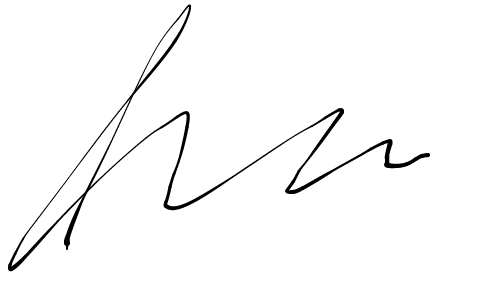
\includegraphics[width=0.35\textwidth]{unterschrift}\vspace*{-0.35cm}
		\\
		\rule[0.5ex]{12em}{0.55pt} & \rule[0.5ex]{12em}{0.55pt} \\
		(Ort, Datum) & (Eigenhändige Unterschrift)
		\\
	\end{tabular*} \\
\end{table}

\newpage


%-----------------------------------
% Seitennummerierung auf arabisch und ab 1 beginnend umstellen
%-----------------------------------
\pagenumbering{arabic}
\setcounter{page}{1}

%-----------------------------------
% Kapitel / Inhalte
%-----------------------------------
% Die Kapitel werden über folgende Datei eingebunden
% Hinzugefügt aufgrund von Issue 167
%-----------------------------------
% Kapitel / Inhalte
%-----------------------------------
\section{Einleitung}
Der Einsatz von Robotern prägt zunehmend den Arbeitsmarkt und beeinflusst die Art und Weise wie Unternehemn ihre Prozesse gestalten. Diese Entwicklung beschränkt sich nicht nur auf die Industrie und den Verbrauchermarkt, sondern immer zunehmender auch auf die Dienstleistungsbranche. So ist der Absatz an Service Robotern für professionelle Anwendungen 2022 laut der International Federation of Robotics \cite{IFR2023} um 48\% gestiegen. Hierbei gibt es laut der \ac{IFR} eine Abgrenzung zu Service Robotern für Verbraucher, bei denen der Absatz 2022 gesunken ist \cite[S.~37]{WorldRobotics2023} und Industrie Robotern bei denen der Absatz 2022 gestiegen ist \cite[S.~9]{WorldRobotics2023}. Aufgrund der Stichprobenentnahme für die Berechnung des Absatzes ist keine genauere Vergleichbarkeit zwischen den Absatzdaten möglich. Das Wachstum des Absatzes wird laut der \ac{IFR} \cite[S.~36]{WorldRobotics2023} unter anderem durch eine gesteigerte Nachfrage getrieben, die auf einen Mangel an Arbeitskräften zurückzuführen ist. Laut der \ac{BA} \cite{BA2024} ist beispielsweise die Menge unbesetzter Arbeitsplätze in Deutschland in den letzten 12 Jahren um ca. zwei Drittel gestiegen und trotz des Rückgangs um ~9\% im Jahr 2023 weiter auf einem hohen Stand. Service Roboter bieten die Möglichkeit diesen Mangel an Arbeitskräften zu mitigieren, da sie eine effiziente Unterstützung der Arbeiter bieten und so die Produktivität erhöhen. Hierbei ersetzen Service Roboter die Menschen meistens nicht vollständig, sondern unterstützen diese nur. Laut Sprenger \cite[S.~272]{Sprenger2015} muss ein Transportroboter beispielsweise von einem Menschen mitgeteilt bekommen was von wo nach wo transportiert werden soll, kann den Transport dafür dann aber vollständig automatisch durchführen.

\subsection{Hintergrund und Motivation}
Insbesondere in der Gastronomie gibt es einen großen Personalmangel. Dieser ist zum Teil auf die Corona-Pandemie zurückzuführen, da in dieser Zeit viele Angestellte in andere Berufsfelder gewechselt. Laut dem Institut der deutschen Wirtschaft \cite{BA2024} - welches sich auf Daten der \ac{BA} bezieht - sind während des Pandemiejahrs 2020 216.000 Arbeiter aus dem Gastgewerbe in ein anderes Berufsfeld gewechselt. Das Gastgewerbe schließt hierbei neben der Gastronomie auch die Hotellerie und Tourismus mit ein. Der Personalmangel macht den Einsatz von Service Robotern in der Gastronomie besonders attraktiv. Diese können dort besonders gut Kellneraufgaben übernehmen und so das Personal entlasten. Das steigert nicht nur die Produktivität, sondern verbessert zusätzlich auch die Arbeitsbedingungen der Kellner. Wie bereits erwähnt agieren die Transportroboter hierbei nicht vollständig autonom, sondern müssen von Menschen ihre Aufträge mitgeteilt bekommen. Man braucht aber nicht nur die Möglichkeit Robotern Aufgaben mitzuteilen, sondern auch die Möglichkeit Roboter zu Orten und herauszufinden was die Roboter aktuell machen.

In dieser Arbeit wird sich speziell mit den Lieferrobotern von Pudu beschäftigt, da diese dem Author zur verfügung stehen. Pudu bietet verschiedene Lieferroboter, an die in der Gastronomie zur Entlastung der Kellner eingesetzt werden können \cite{PUDU2024}. Für diese Arbeit wird auf eine bereits entwickelte API zurückgegriffen, die Endpunkte bereitstellt, mit denen unteranderem Lieferaufträge gegeben und Daten der Roboter abgerufen werden können.

% Im Zuge der weiteren Vertiefung dieses Themas wird im Verlauf der Arbeit genauer auf die Rolle von Service Robotern als Antwort auf den Fachkräftemangel eingegangen. Hierbei werden nicht nur die Vorteile, sondern auch die Herausforderungen und mögliche Lösungsansätze beleuchtet, um eine umfassende Perspektive auf die Thematik zu gewährleisten.

\subsection{Zielsetzung und Forschungsfrage}
Diese Arbeit setzt an dem Punkt an und verfolgt entsprechend das Ziel eine Anwendung zu konzeptionieren und prototypisch zu implementieren, die die Möglichkeit bietet Service Roboter in der Gastronomie zu steuern und zu verwalten. Diese Anwendung soll eine intuitive Steuerung und Übersicht bieten. Bei der Anwendung soll es sich aufgrund verschiedener Vorteile gegenüber nativen Apps um eine Webanwendung handeln. So können Webanwendungen plattformunabhängig genutzt werden und sind sofort ohne Download und Installation verfügbar. Da diese Anwendung in beliebigen Gastronomiebetrieben einsetzbar sein soll, braucht es hierfür auch eine Visualisierung des entsprechenden Gebäudes. Für eine bessere übersichtlichkeit soll diese visualisierung 3-dimensinal sein. Das Erstellen eines 3D Modells erfordert klassischerweise technisches Know-How in Modellierungssoftware wie beispielsweise Blender. Dieses fehlt in den meisten Gastronomiebetrieben, weshalb hierfür eine einfacherere Lösung gefunden werden soll. Das Generieren einer 3-dimensionalen Gebäudeübersicht ist entsprechend ein zusätzlicher Schwerpunkt dieser Arbeit.

Aus dieser Zielsetzung ergibt sich die folgende Forschungsfrage: Wie kann eine effiziente und benutzerfreundliche Steuerung und Verwaltung von Servicerobotern implementiert werden? Ein besonderer Schwerpunkt liegt hierbei auf der Ausarbeitung einer Methode zur einfachen Generierung von 3D-Modellen, um die Grundlage für die nutzerfreundliche Visualisierung und Navigation in der Webanwendung zu schaffen. Die ausgearbeitete Methode muss nicht zwingend in die Webanwendung integriert werden, sondern kann lediglich ein 3D-Modell generieren, welches dann in der Webanwendung importiert werden kann.

\subsection{Methodik}
Diese Arbeit orientiert sich an dem \ac{DSR} Ansatz nach Hevner. Dieser bietet speziell einen Rahmen für \ac{DSR} im Bereich der Informationssysteme. Grundsätzlich ist \ac{DSR} ein iterativer Forschungsansatz, mit dem Lösungen für praktische Probleme, mithilfe der Entwicklung von Artefakten gefunden werden. In dem Fall dieser Arbeit ist das Artefakt die Webanwendung, die konzeptioniert und prototypisch implementiert werden soll. 

\subsubsection{Design Science Research nach Hevner}
Bei diesem Unterkapitel handelt es sich um eine Zusammenfassung des \ac{DSR} Ansatz nach Hevner \cite[S.~79-81]{Hevner2004}. Hevners Ansatz besteht aus verschiednene Zyklen:

\begin{itemize}
    \item Relevancy Cycle
    \item Rigor Cycle 
    \item Design Cycle
\end{itemize}

Mit diesen Zyklen wird eine systematische Entwicklung und Bewertung der Artefakte erreicht. Hevners Ansatz berücksichtigt die Umgebung, in der und für die das Artefakt entwickelt wird und die Wissensgrundlage, auf der das Artefakt aufbaut. Diese Wissensgrundlage wird durch die Entwicklung des Artefakts erweitert. Im Folgenden werden die Zyklen, Umgebung und Wissensgrundlage genauer erklärt.

\begin{itemize}
    \item Die Umgebung besteht aus den relevanten Menschen, Organisationen und Technologien. Sie definiert den Problemraum in dem geforscht wird. Aus der Umgebung ergeben sich die organisatorischen Bedürfnisse beziehnungsweise das Problem, dass gelöst werden soll und die Anforderungen an die Lösung.
    \item Die Wissensgrundlage bietet verbildlicht die Rohmaterialien mit denen der Design Cycle durchgeführt werden kann. Im Fall dieser Arbeit bezieht sich das beispielsweise auf mögliche Frameworks mit denen 3D-Modelle in der Webanwendung eingebunden werden können, aber auch auf Methoden für die Auswertung des Prototyps.
    \item Im Design Cycle, wird das Artefakt iterativ entwickelt und ausgewertet. Mithilfe des Relevancy Cylce wird sichergestellt, dass das Artefakt das ursprüngliche Problem löst. Der Rigor Cycle bietet eine Wissensgrundlage auf der aufbauend entwickelt werden kann.
    \item Im Relevancy Cycle wird das Problem beziehungsweise die Anforderungen die sich aus dem Problem ergeben an den Design Cycle übergeben. Das Artefakt, das im Design Cycle entsteht, wird dann in der Umgebung getestet. Hierdurch wird sichergestellt, dass das Artefakt das entsprechende Problem in der Umgebung auch wirklich löst.
    \item Im Rigor Cycle wird die Wissensgrundlage an den Design Cycle übergeben. Mit der Entwicklung des Artefakts entsteht neues Wissen. Dieses erweitert die Wissensbasis. Der zweite Teil des Rigor Cycle ist somit nur für die zukünftige Anwendung relevant.
\end{itemize}

\subsubsection{Einsatz im Rahmen der Arbeit}

Die verschiedenen Schritte des \ac{DSR} Ansatz nach Hevner werden in dieser Arbeit mithilfe verschiedener Methoden abgewandelt.

\paragraph{Literaturrecherche}

Im ersten Schritt wird eine systematische Literaturrecherche durchgeführt. Mit dieser soll das grundlegende Verständnis über die Umgebung geschaffen werden. So soll insbesondere Wissen zu den Service Robotern gesammelt werden, die in der Gastronomie eingesetzt werden können. Mithilfe der Literaturrecherche soll außerdem die Wissensbasis geschaffen werden. Insbesondere soll Wissen gesammelt werden, mit dem sich eine Lösung für die Generierung von 3D-Modellen von Gebäuden finden lässt. Außerdem soll Wissen zur Einbindung von 3D-Modellen im Web gesammelt werden. Während der Implementierung des Prototyps werden außerdem wahrscheinlich weitere größere technische Probleme auffallen, für die dann entsprechend Wissen gesammelt werden muss. Entsprechend beschränkt sich der Schritt der Literaturrecherche nicht auf den Beginn der Arbeit. Stattdessen wird sie mit dem Auftreten neuer technischer Probleme wiederholt relevant sein.

\paragraph{Anforderungsanalyse}

Daraufhin wird auf Basis des Wissens zur Umgebung im Kontext der Forschungsfrage eine Anforderungsanalyse für den Prototyp erstellt. Durch die Forschungsfrage und den festgelegten Schwerpunkt (3D-Modelle von Gebäuden) stehen bereits verschiedene funktionale und nicht-funktionale Anforderungen fest. So existieren bereits folgende funktionale Anforderungen:

\begin{itemize}
    \item Es soll eine Webanwendung implementiert werden.
    \item Die Anwendung soll eine 3-dimensionale Visualisierung der entsprechenden Gebäude bieten.
\end{itemize}

\begin{samepage}
Außerdem existieren bereits folgende nicht-funktionale Anforderungen:

\nopagebreak
\begin{itemize}
    \item Die Anwendung soll benutzerfreundlich sein.
    \item Die Anwendung soll effizient sein.
\end{itemize}
\end{samepage}

Hierbei muss allerdings basierend auf dem Wissen zur Umgebung noch genauer definiert werden, was unter den beiden Begriffen genau zu verstehen ist. So sollte  präzisiert werden welche Aspekte der Benutzerfreundlichkeit wichtig sind und welche Art von Effizienz gemeint ist.

\paragraph{Umsetzung}

Basierend auf den gesammelten Anforderungen ergeben sich größere technische Herausforderungen. Wie bereits erwähnt sind verschiedene technische Herausforderungen bereits abzusehen, die mithilfe der Wissensbasis gelöst werden sollen. Während der Implementierung des Prototyps können, wie bereits beschrieben weitere Herausforderungen auftreten die mithilfe der sich kontiluierlich entwickelnden Wissensbasis gelöst weren können.

Sobald die Anforderungen definiert sind und die ersten technischen Herausforderungen gelöst sind kann mit der Implementierung des Prototyps begonnen werden. Dieser soll im Verfahren des Rapid Prototypings entwickelt werden, bei denen sich die Implementierung und Evaluierung iterierend abwechseln. Die Benutzerfreundlichkeit und Effizienz des Prototyps soll hierbei durch Usability Tests und Performance Tests evaluiert werden.

\paragraph{Usability Tests}
% Usability Tests kurz erklären
% Während einem Großteil der Implementierung nur kleinere inoffizielle Tests durch den Entwickler durchgeführt um Probleme zu finden
% Zum Ende Usability Tests durch ausgewählte Testpersonen
    % Dadurch wird Zeit gespart, da Usability Tests zeitlich aufwändig sind. So wurde versucht die meisten größeren Probleme schon vorher zu finden.
    % praktisch ein groberer Filter während der Implementierung der weniger Zeit kostet, und dann ein (oder mehrere) feinere Filter zum Ende der Implementierung.

\paragraph{Performance Tests}

\newpage
\section{Grundlagen}\label{Grundlagen}
In diesem Kapitel werden grundlegende Konzepte und Technologien in den Bereichen Serviceroboter, Webanwendungen, 3D-Modelle und Softwarequalität vorgestellt.

\subsection{Serviceroboter}
Dieser Abschnitt gibt einen kurzen Überblick über Serviceroboter im Allgemeinen und eine Einführung in die Funktionen der Roboter, die im Prototyp eingesetzt werden. Außerdem wird das \ac{BCB} genauer erläutert.

\subsubsection{Definition}
Nach der ISO Norm 8373:2021 handelt es sich bei Servicerobotern um Roboter, die im privaten oder professionellen Gebrauch für Menschen nützliche Aufgaben erledigen. Serviceroboter werden hierbei von Industrierobotern und Medizinrobotern abgegrenzt. Roboter müssen zudem voll- oder zumindest teilautonom handeln können.\cite[S.~1-2]{ISO2021} Unter dem professionellen Gebrauch versteht man den kommerziellen Einsatz \cite[S.~4]{GonzalezAguirre2021}, unter anderem im Gesundheitswesen, in der Landwirtschaft oder im Tourismus \cite[S.~9]{GonzalezAguirre2021}.

\subsubsection{Einsatzmöglichkeiten}
Serviceroboter werden bereits vielfältig professionell eingesetzt. So gibt es verschiedene Beispiele in denen sie in Hotels für den Gästeempfang, den Check-in und die Gepäcklieferung und an Flughäfen für die Beratung von Reisenden, das Scannen von Boardingpässen, den Check-in, die Bodenreinigung und Patrouillengänge genutzt werden \cite[S.~425]{Paluch2020}. In der Pflege können Serviceroboter den Pflegern beim Heben von Patienten und beim Durchführen von Übungen mit Patientengruppen aushelfen \cite[S.~427]{Paluch2020}. Aufgaben mit geringer kognitiver und emotionaler Komplexität können in der Regel vollautonom und ohne Aufsicht eines Menschen durchgeführt werden \cite[S.~429]{Paluch2020}. Unter solche Aufgaben fällt zum Beispiel Staubsaugen, Rasenmähen und Gepäcklieferung. Komplexere Aufgaben erfordern die Aufsicht oder Unterstützung von Menschen, wodurch diese nur teilautonom ausgeführt werden \cite[S.~430-431]{Paluch2020}. Für den Einsatz von Servicerobotern müssen immer die Vor- und Nachteile abgewogen werden. So können zum Beispiel Roboter, die im Kontakt mit Kunden eingesetzt werden, Emotionen vorspielen, die von Kunden allerdings als unauthentisch erkannt werden. Gleichzeitig sind Roboter im Gegensatz zu Menschen dafür ununterbrochen freundlich.\cite[S.~427]{Paluch2020}

\subsubsection{Pudu Robotics}
Der Prototyp wird für den Einsatz von Pudu Robotern konzipiert. Pudu stellt Serviceroboter her, die vor allem in der Gastronomie eingesetzt werden können. Die Modelle sind hierbei auf unterschiedliche Funktionen, wie das Begrüßen von Gästen, das Liefern bestellter Speisen, das Zurückbringen dreckigen Geschirrs und das Putzen des Bodens spezialisiert \cite{PUDU2024}. Damit die Roboter diese Funktionen ausführen können, müssen sie eigenständig durch komplexe, sich ändernde Umgebungen navigieren. Die eigenständige Navigation lässt sich in die Teilfunktionen Positionsfindung, Wahrnehmung und Routenplanung aufteilen, wobei die Positionsfindung eine Schlüsselrolle spielt \cite[S.~1]{Nature2022}. Zur Positionsfindung erstellen sich die Pudu Roboter mit dem sogenannten \ac{VSLAM} eine Karte ihrer Umgebung, was bei einer Fläche von 1000 Quadratmetern eine Stunde dauern kann. Während Roboter zur Navigation normalerweise platzierte Markierungen benötigen, können sich Pudu Roboter mithilfe einer nach oben gerichteten Kamera anhand der Zimmerdecke orientieren.\cite{Pudu2023} Durch weitere Kameras und Sensoren können die Roboter außerdem ihre Umgebung wahrnehmen \cite[S.~1]{Nature2022}.

\subsubsection{Bot Control Backend}\label{sec:BotControlBackend}
Das bereits existierende \ac{BCB} wird als Schnittstelle zwischen den Pudu Robotern und dem Prototyp genutzt. Über dieses können die Roboter zum Beispiel beauftragt werden. Die folgenden Informationen zum Service Framework der Roboter stammen aus dem SDK Guidance Document \cite{PuduSDK}, das der Tobit Laboratories AG, für die Entwicklung des \ac{BCB}s, durch Pudu zur Verfügung gestellt wurde.

Die Abbildung \ref{fig:BotControlBackendCommunication} veranschaulicht die Kommunikation zwischen dem \ac{BCB} und den Robotern. Wie man in der Abbildung sieht hat das \ac{BCB} eine direkte Verbindung zum \gls{Microservice}, der wiederum über die PUDU Cloud – die als \gls{MQTT-Broker} agiert – mit den Robotern kommuniziert. Über \gls{HTTP}-Anfragen an den \gls{Microservice} können Daten abgefragt und Befehle gegeben werden. Bei der Anfrage von Daten fragt der \gls{Microservice} die entsprechenden \gls{MQTT}-Topics an. Wie die Kommunikation zwischen \gls{Microservice} und Robotern genau funktioniert, wenn das \ac{BCB} Befehle an die Roboter verschickt, ist aus dem Dokument nicht ersichtlich. Die Roboter können zusätzlich auch unaufgefordert Ereignisse an das \ac{BCB} kommunizieren. Hierfür muss das \ac{BCB} eine Adresse für einzelne Ereignistypen im \gls{Microservice} als \gls{Webhook} registrieren. Der \gls{Microservice} abonniert daraufhin die entsprechende \gls{MQTT-Topic}. So schicken die Roboter auftretende Ereignisse – wie eine Positionsaktualisierung – an die PUDU Cloud, die diese an den \gls{Microservice} weiterleitet, da dieser die \gls{MQTT-Topic} abonniert hat. Der \gls{Microservice} schickt das Ereignis daraufhin als \gls{HTTP}-Nachricht an die, als \gls{Webhook} registrierte, Adresse im \ac{BCB}.

\begin{figure}[H]
    \caption{Kommunikation zwischen Bot Control Backend und Robotern}\label{fig:BotControlBackendCommunication}
    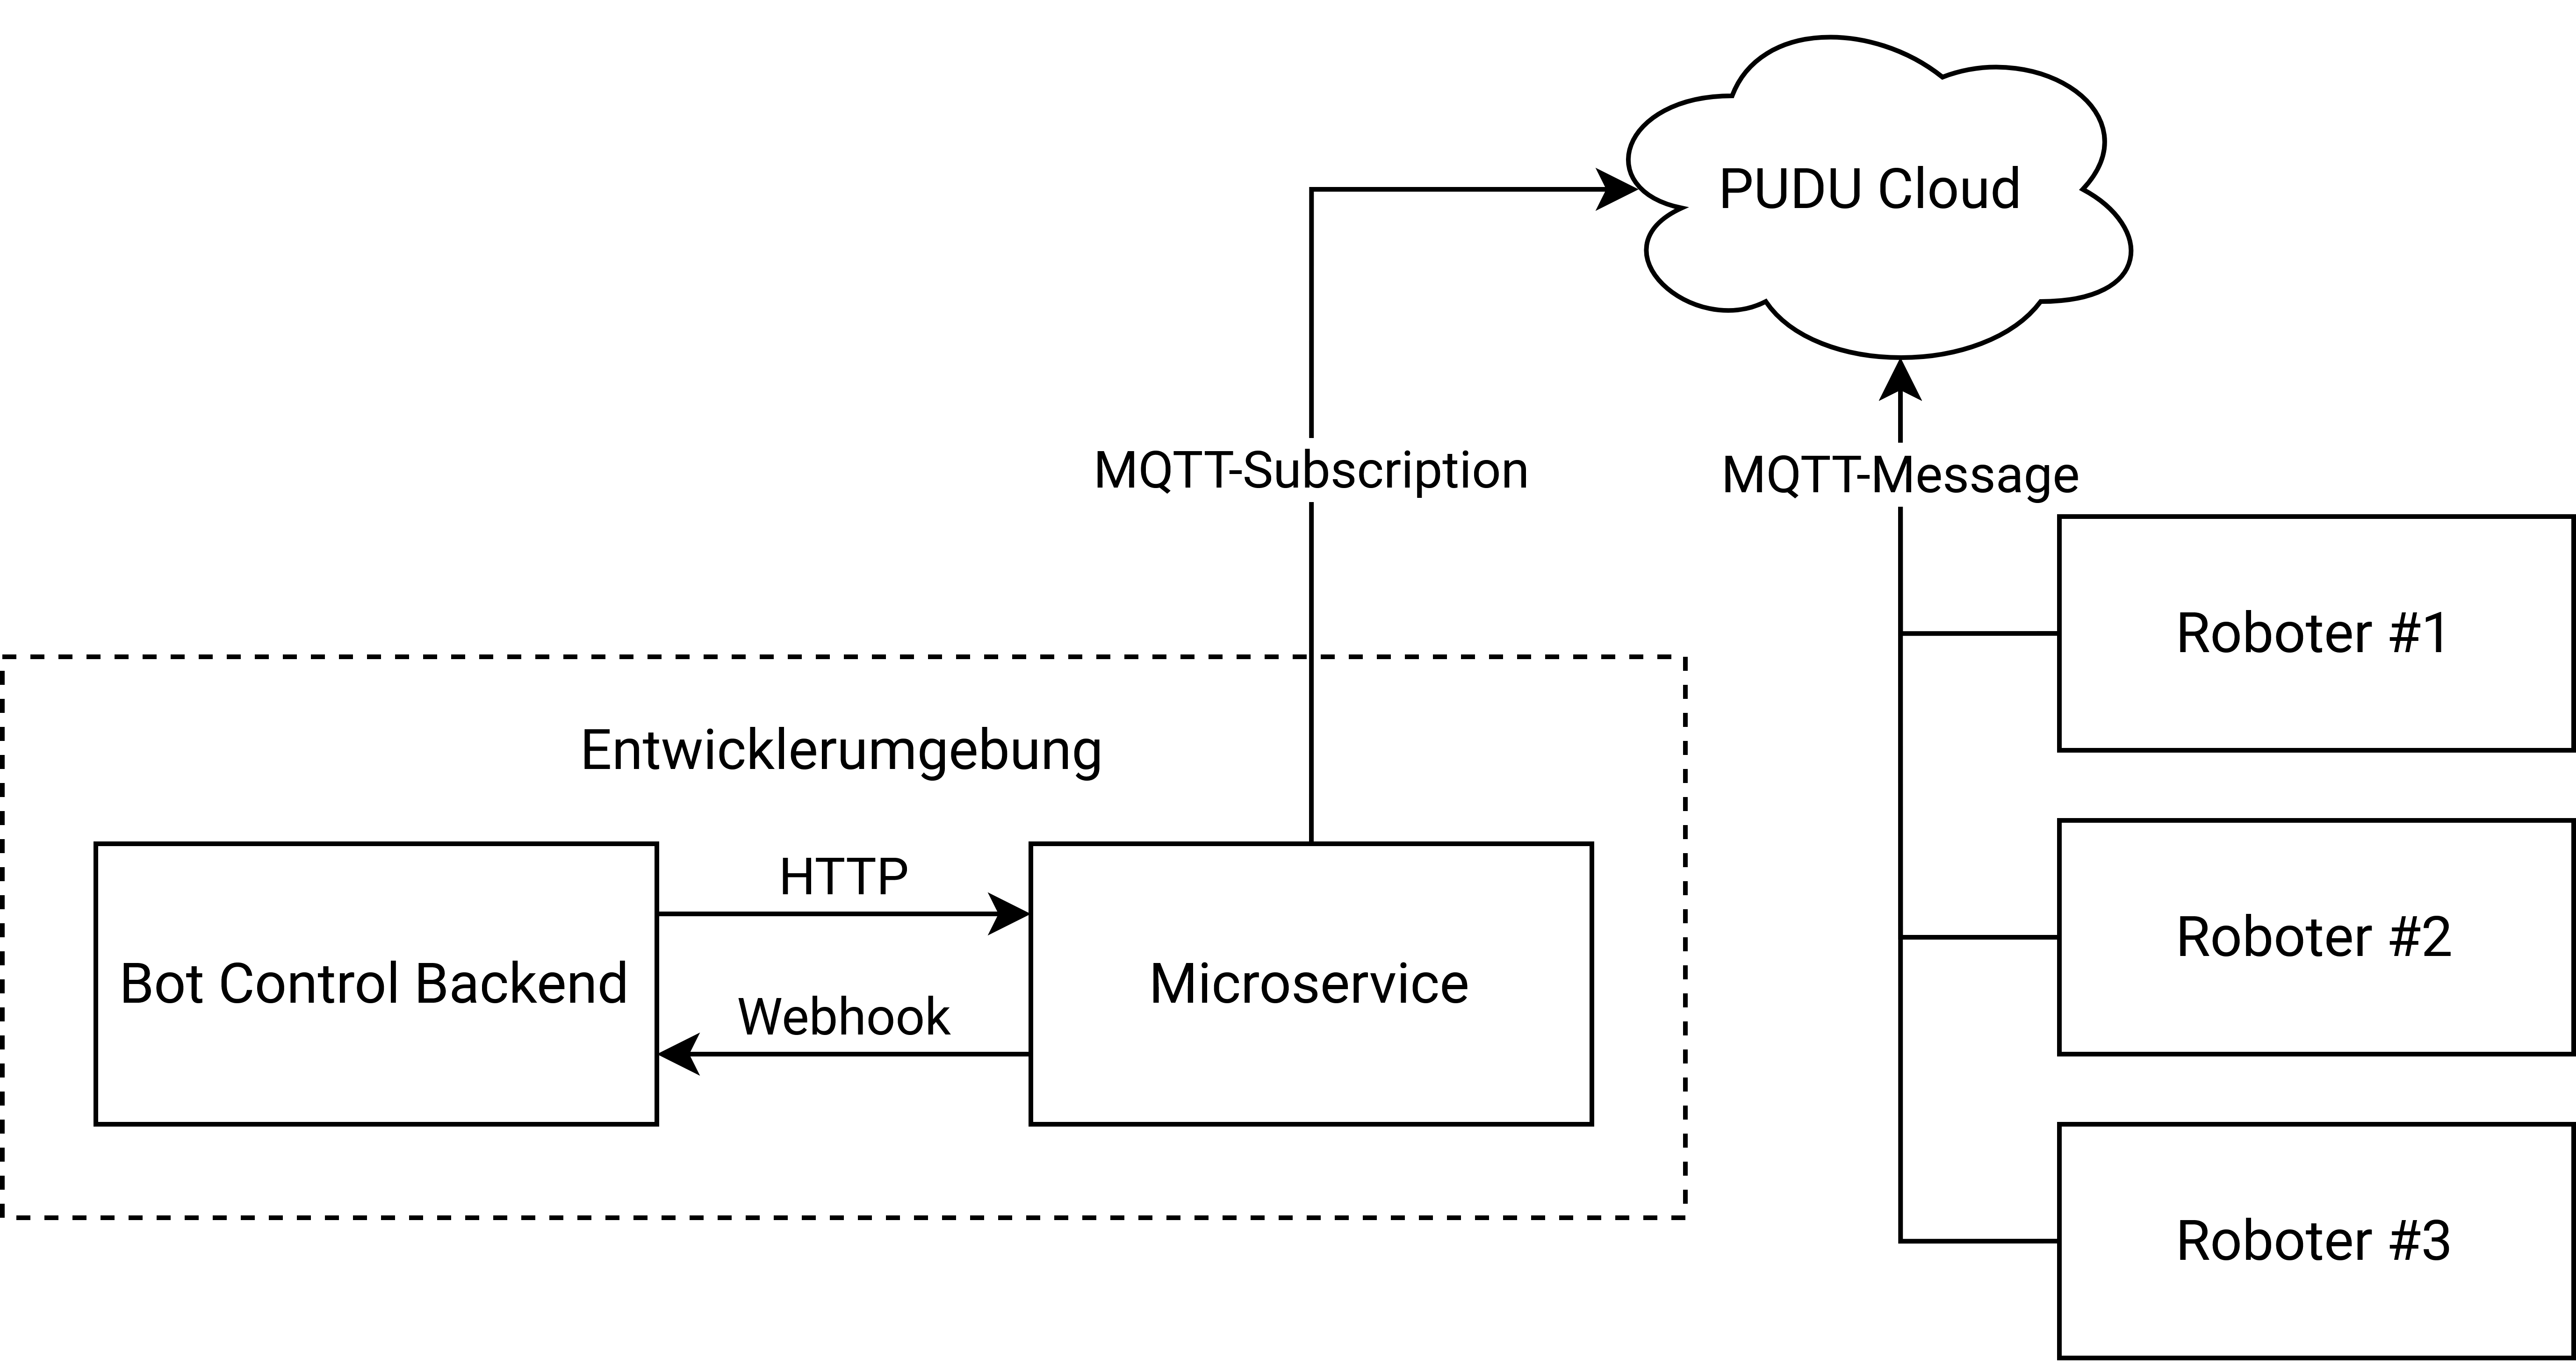
\includegraphics[width=0.9\textwidth]{BotControlBackend Diagramm2}
    \\
    Quelle: In Anlehnung an Pudu \cite[S.~4]{PuduSDK}
\end{figure}

Das \ac{BCB} fungiert nicht nur als Kommunikationsschnittstelle zu den Robotern, sondern abstrahiert auch neue Funktionen. So können Roboter mithilfe des \ac{BCB}s Fahrstuhl fahren und somit Lieferpunkte in anderen Stockwerken erreichen. Ebenso können sie durch das \ac{BCB} an geschlossenen Türen halten, diese öffnen und anschließend weiterfahren.

Es gibt verschiedene Daten, die über das \ac{BCB} abgerufen werden können und für den Prototyp relevant sind, wie die Position der Roboter innerhalb ihrer internen Karte, sowie die Positionen wichtiger Standorte, wie Lieferpunkte und Ladestationen. Außerdem sind auch die Pfade relevant, an denen sich die Roboter während der Fahrt orientieren. Darüber hinaus sind auch noch die Positionen der virtuellen Wände wichtig. Diese müssen manuell platziert werden und agieren aus der Sicht der Roboter wie echte Wände, wodurch sichergestellt wird, dass bestimmte Bereiche nie durchfahren werden.

\subsection{Webanwendungen}
Webanwendungen sind Softwareanwendungen, die auf Webservern gehostet werden und über Webbrowser aufgerufen werden können. Sie ermöglichen es Benutzern über das Internet auf Anwendungen zuzugreifen, ohne dass eine Installation dieser erforderlich ist. Da sie auf verschiedenen Betriebssystemen und Gerätetypen verwendet werden können, solange ein kompatibler Webbrowser zur Verfügung steht, sind sie plattformunabhängig nutzbar.\cite[Abschnitt~1-2]{AWSWebApp} Zusammenfassend sind Webanwendungen breit und einfach zugänglich.

\subsubsection{Technologien und Softwarebibliotheken}\label{sec:WebTechnologies}
Die reibungslose Entwicklung ansprechender Webanwendungen erfordert den Einsatz verschiedener Technologien.

Die drei zentralen Technologien jeder Webanwendungen sind \ac{HTML}, \ac{CSS} und JavaScript. \ac{HTML} ist eine Auszeichnungssprache, die die Struktur einer Webseite definiert, indem Elemente wie Überschriften, Absätze und Hyperlinks verwendet werden, um Inhalte zu organisieren und zu strukturieren \cite{HTML}. Um das Erscheinungsbild einer Webseite zu gestalten wird \ac{CSS} genutzt. Mit \ac{CSS} lassen sich Layout, Formatierung und weitere Eigenschaften von \ac{HTML}-Elementen definieren.\cite{CSS} \ac{Sass} erweitert \ac{CSS} durch Verschachtelung, Variablen, \gls{Mixins} und weitere Funktionen \cite{Sass}, wodurch die Wiederverwendbarkeit definierter Styles verbessert und die Entwicklung vereinfacht wird. Die Interaktivität von Webseiten wird durch JavaScript ermöglicht \cite{JavaScript}. Bei JavaScript handelt es sich um eine dynamisch typisierte Skriptsprache, die durch TypeScript um eine statische Typisierung erweitert wird \cite{TypeScript}. Durch TypeScript wird die Entwicklung einer robusten und fehlerfreien Webanwendung im Vergleich zu JavaScript erleichtert.

Die Entwicklung komplexerer Webanwendungen wird durch die JavaScript-Bibliotheken React und Redux weiter erleichtert. React wird zur Erstellung von Benutzeroberflächen verwendet und ermöglicht die Entwicklung wiederverwendbarer \ac{UI} Komponenten – im Folgenden auch React-Komponenten genannt –, sowie eine effiziente Aktualisierung der Benutzeroberflächen durch die Verwendung virtueller \gls{DOM}s. React-Projekte werden in \ac{JSX} entwickelt, womit sich \ac{HTML} Elemente im JavaScript-Code integrieren lassen. Damit React Projekte von Webbrowsern ausgelesen werden können, muss der geschriebene \ac{JSX}-Code zu JavaScript transpiliert werden.\cite{React} Redux ermöglicht eine übersichtliche Verwaltung des Anwendungsstatus \cite{Redux}.

\subsubsection{chayns}\label{sec:Chayns}
Bei chayns handelt es sich um eine Digitalisierungsplattform, die durch die Tobit Software GmbH vertrieben wird. Unter anderem bietet chayns einen Cloud-Speicher – den chayns.space – und einen Webseiten-Baukasten, mit dem sich Nutzer eine Webpräsenz erstellen können. Auf den Webseiten können vordefinierte chayns Anwendungen, wie ein eShop oder ein Bundesliga-Tippspiel, aber auch eigenentwickelte Webanwendungen eingebunden werden.\cite{chayns} Als Besitzer einer chayns Seite hat man Zugriff auf den Admin-Modus, in dem sich die meisten chayns Anwendungen verwalten lassen. So gibt es auch im entwickelten Prototyp eine Nutzer- und Adminansicht. Tobit bietet verschiedene Softwarebibliotheken, die die Entwicklung von chayns Anwendungen erleichtern. So gibt es den Shell Befehl create-chayns-app \cite{CreateChaynsApp}, mit dem chayns basierte React Projekte aufgesetzt werden können; das \ac{npm} Paket chayns-toolkit \cite{ChaynsToolkit}, mit dem chayns basierte React Projekte kompiliert werden können; das \ac{npm} Paket chayns-components \cite{ChaynsComponents}, das React-Komponenten für verschiedene \ac{GUI} Elemente zur Verfügung stellt; und das \ac{npm} Paket chayns-api \cite{ChaynsApi}, das verschiedene hilfreiche Funktionen bereitstellt. Für unternehmensinterne Projekte bietet Tobit den \gls{Websocket}-Service der eine indirekte \gls{Websocket}-Verbindung zwischen Backends und Clients ermöglicht. Über diese können Backends unaufgefordert Nachrichten an verbundene Clients versenden.

\subsection{3D Modelle}
Dieser Abschnitt bietet eine kurze Einführung in das Thema der 3D-Modelle. Daraufhin werden verschiedene Methoden zur Erzeugung von 3D-Gebäudemodellen vorgestellt und es wird erläutert, wie 3D-Modelle in Webanwendungen eingebunden werden können.

3D-Modelle sind digitale Darstellungen von Objekten oder Szenen in drei Dimensionen. Anders als bei 2D-Grafiken, die lediglich eine Breite und Höhe haben, enthalten 3D-Modelle zusätzlich Tiefeninformationen, aus denen sich die dritte Dimension ergibt. Polygonale 3D-Modelle bestehen aus Polygonen, die sich aus Eckpunkten und Kanten – den Verbindungen zwischen Eckpunkten – zusammensetzen. Oberflächeneigenschaften der Polygone, wie Farben, Glanz und Reflexionen lassen sich durch die Anwendung von Texturen und Materialien definieren. Transformationsoperationen wie Skalierung, Rotation und Translation ermöglichen es, 3D-Modelle im Raum zu bewegen und zu manipulieren. Die Kamera, Perspektive und Projektion legen den Standpunkt des Betrachters und die Darstellung des Modells fest.\cite[S.~8-16]{Parisi2014}

\subsubsection{Generierung}
Neben der manuellen Modellierung von 3D-Modellen, mithilfe von Modellierungssoftware wie Blender \cite{Blender}, gibt es verschiedene Methoden, die sich insbesondere zur Generierung von Raummodellen eignen.

\paragraph{Fotogrammetrie}

Die Fotogrammetrie beschäftigt sich damit, Messungen aus einer Vielzahl an zweidimensionalen Bildern abzuleiten, aus denen sich präzise 3D-Modelle erzeugen lassen \cite[S.~19]{Aber2010}. Inzwischen erfordert die Fotogrammetrie nicht mehr den Einsatz teurer Kameras, da die Kameras moderner Mobilgeräte eine ausreichende Bildqualität bieten \cite{Cohrs2021}. Bei der Planung und Durchführung der Bildaufnahmen müssen verschiedene Aspekte beachtet werden. Innerhalb der aufzunehmenden Szene sollte es eine gleichmäßige Belichtung, möglichst keine reflektierende oder transparente Flächen und keine sich bewegende Objekte geben. Während der Aufnahme müssen Parameter wie Belichtungszeit und Weißabgleich passend konfiguriert sein und zwischen den einzelnen Aufnahmen unverändert bleiben. Außerdem muss sich der Inhalt aufeinanderfolgender Bilder stets überschneiden.\cite{Cohrs2021b} Nach der Durchführung der Aufnahmen erfolgt die Verarbeitung mithilfe spezialisierter Software, deren Bedienung komplex sein kann. Für eine reibungslose Verarbeitung sind eine leistungsstarke \ac{GPU} und ausreichend Speicherplatz unerlässlich.\cite{Cohrs2021c}

\paragraph{LiDAR Scanning}
Im Gegensatz zur Fotogrammetrie nutzt \ac{LiDAR} einen aktiven Sensor. Es wird Licht in Form eines pulsierenden Lasers ausgesendet. Die Reflexionen werden mit einem Scanner erfasst, wodurch sich Abstände zwischen Sensor und Gegenständen berechnen lassen. Auf Grundlage dieser Messungen wird ein 3D-Modell erstellt. Wie bei der Fotogrammetrie, muss beim Scannen darauf geachtet werden, dass reflektierende oder transparente Flächen, sowie sich bewegende Objekte vermieden werden. Seit 2020 werden \ac{LiDAR}-Scanner in iOS-Geräte von Apple integriert, was unter anderem zu einer verbesserten Bildqualität beim Fotografieren beitragen soll \cite{Fenstermaker2022}. Als glücklicher Nebeneffekt wurden verschiedene Apps, wie Canvas \cite{Canvas2023}, Polycam \cite{Polycam2024} und Scaniverse \cite{Scaniverse2024} entwickelt, die den \ac{LiDAR}-Scanner nutzen, um 3D-Modelle zu erstellen. Diese Apps versprechen eine schnelle und einfache Erzeugung akkurater 3D-Modelle.

\paragraph{KI gestützte Methoden}
Es existieren verschiedene \ac{KI}-Modelle, die darauf trainiert sind, 3D-Gebäudemodelle mit nur wenigen Bildern zu erzeugen. Eines dieser \ac{KI}-Modelle ist Plan2Scene. Es benötigt als Eingabe einen Grundriss des Gebäudes, sowie Bilder, die den einzelnen Räumen zugeordnet sind. Basierend auf dem Grundriss generiert das \ac{KI}-Modell ein 3D-Modell mit Möbeln. Basierend auf den Bildern der Räume werden monotone Texturen generiert.\cite[S.~10733]{Plan2Scene2021} Das Rent3D Modell funktioniert ähnlich, nutzt die Bildaufnahmen aber direkt als Textur, statt sie aus den Bildaufnahmen zu generieren \cite[S.~3413]{Rent3D2015}.

\subsubsection{Einbindung im Web}
Das Einbinden von 3D-Modellen wird im Web durch die \ac{WebGL} und WebGPU ermöglicht. Während \ac{WebGL} für lange Zeit der etablierte Standard war, gewinnt WebGPU seit der Veröffentlichung im Jahr 2021 stetig an Popularität.

\paragraph{WebGL und WebGPU}
\ac{WebGL} wurde 2011 von der Khronos Group entwickelt und ist ein JavaScript \ac{API} mit dem 3D-Grafiken im Webbrowser ohne den Einsatz zusätzlicher Plugins dargestellt werden können. Die 3D-Grafiken können hierbei hardwarebeschleunigt angezeigt werden, also mithilfe spezialisierter Hardware wie einer \ac{GPU}. Durch die Integration mit \ac{HTML} und JavaScript können 3D-Grafiken dynamisch auf Webseiten eingebunden werden. Da \ac{WebGL} auf offenen Webstandards basiert, ist es in allen Browsern plattformunabhängig nutzbar.\cite[S.~17-19]{Parisi2014} WebGPU bietet wie \ac{WebGL} das hardwarebeschleunigte Anzeigen von 3D-Grafiken und darüber hinaus eine verbesserte Leistung sowie einen erweiterten Funktionsumfang \cite{Surma2022}. Entwicklern steht eine Vielzahl an Frameworks zur Verfügung die auf \ac{WebGL} oder WebGPU basieren \cite{Seguin2024} und die Entwicklung vereinfachen und beschleunigen.

\paragraph{\deckgl{}}
Das Framework \deckgl{} wurde 2016 von Uber als Open Source Projekt veröffentlicht \cite{Visgl}. Das Framework basiert auf \ac{WebGL}, wobei ab der kommenden Version 9.0.0 stattdessen WebGPU genutzt wird \cite{Green2022}. Mit \deckgl{} lassen sich hochperformante interaktive Karten und Geovisualisierungen mit tausenden bis Millionen Datenpunkten im Web einbinden. Da das Framework auf React ähnlichen Programmierparadigmen basiert, eignet es sich besonders gut für die Einbindung in React Anwendungen. Das Framework funktioniert nach dem \ac{PIL} Prinzip. So gibt es Ebenen, welche grundlegende visuelle Elemente – im Englischen Primitives –, wie Kreise, Rechtecke und Linien, aber auch komplexere teilweise dreidimensionale Elemente nutzen, um Datenpunkte darzustellen. Die Elemente werden in einer Ebene auf Basis der Attribute der Datenpunkte positioniert, skaliert und gefärbt. Die Ebenen können gestapelt und somit kombiniert werden, was auch die Inspiration für den Namen des Frameworks ist, da das englische Wort deck in etwa Stapel bedeuten kann.\cite[S.~2]{YangWang2019} Das Framework bietet verschiedene vordefinierte Ebenen, wie die IconLayer \cite{DeckglIconLayer}, die Icons als grundlegendes visuelles Element nutzt. Zur Veranschaulichung des \ac{PIL}-Prinzips zeigt die Abbildung \ref{fig:IconLayerExample} wie die IconLayer – in Kombination mit einer weiteren Ebene zur Darstellung der Weltkarte – genutzt wird, um die Positionen aller bekannten Meteoritenlandungen auf der Erde anzuzeigen.

\begin{figure}[H]
    \caption{IconLayer Beispiel}\label{fig:IconLayerExample}
    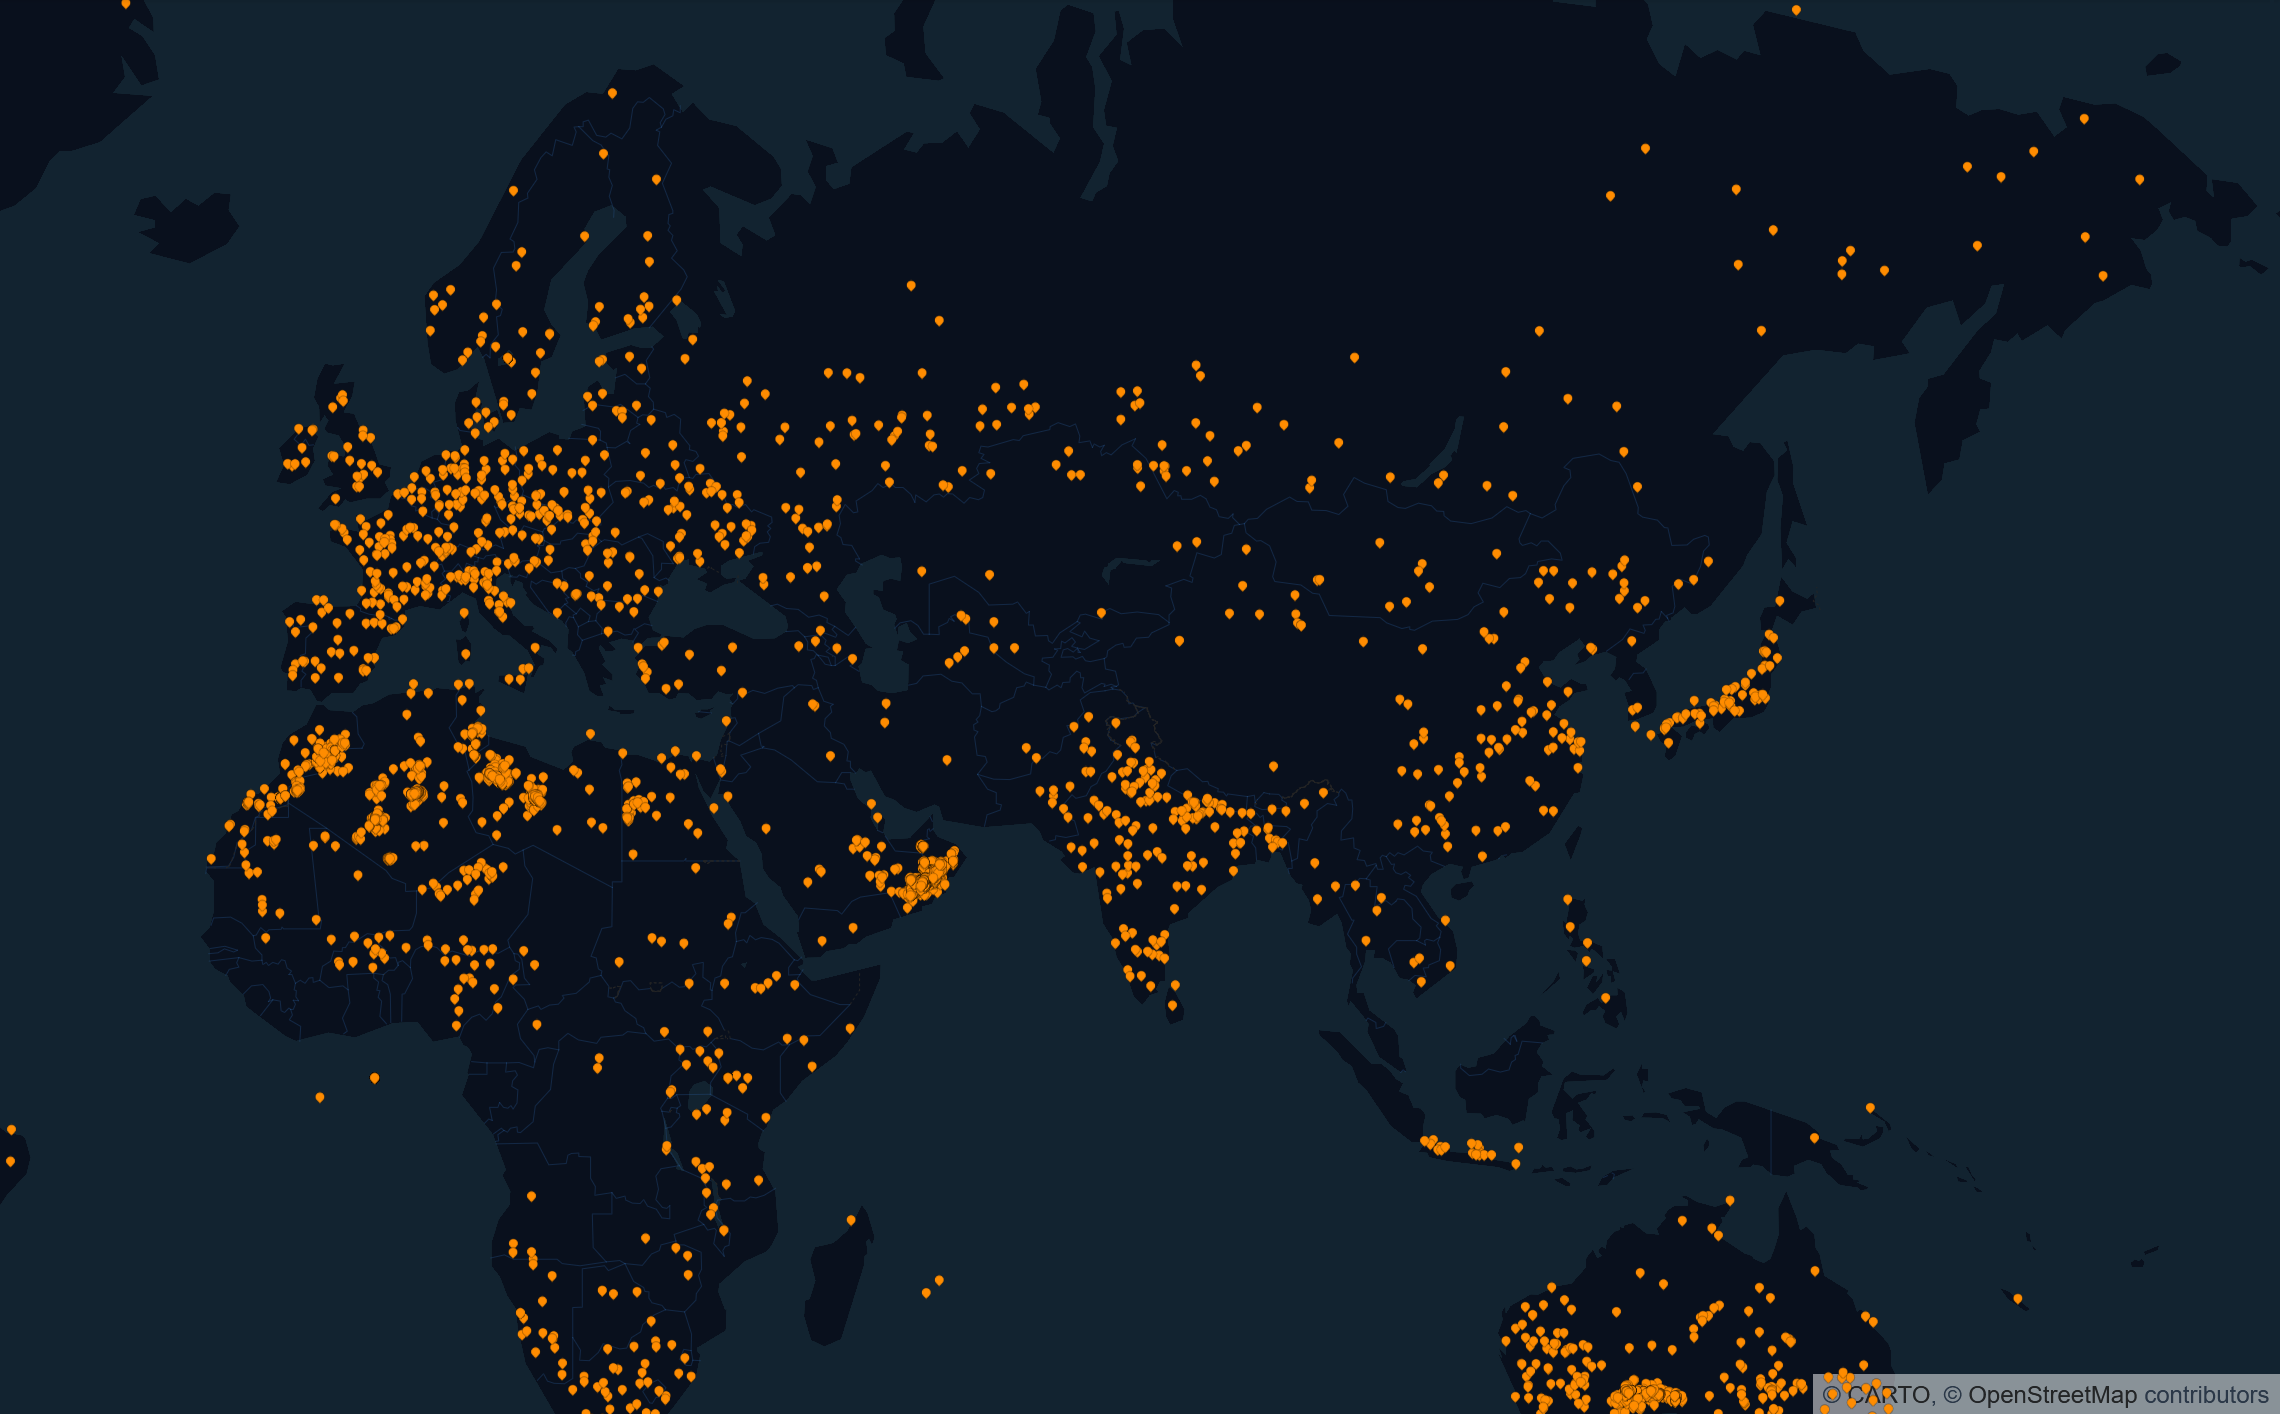
\includegraphics[width=0.9\textwidth]{IconLayer Example.png}
    \\
    Quelle: OpenJS Foundation \cite{DeckGlMeteorites}
\end{figure}

Weitere Ebenen, die für den Prototyp relevant sind, sind die SimpleMeshLayer \cite{DeckglSimpleMeshLayer} und ScenegraphLayer \cite{DeckglScenegraphLayer} für das Anzeigen von 3D-Modellen und die PathLayer für das Anzeigen von Pfaden. \deckgl{} ermöglicht außerdem den Einsatz eigenentwickelter Ebenen, was für den Prototyp aber nicht gebraucht wird. Weitere wichtige Elemente die \deckgl{} bietet sind die Controller Klasse \cite{DeckglController}, mit der die Navigation auf der Karte konfiguriert werden kann und die Viewport Klasse \cite{DeckglViewport}, mit der die Navigation direkt kontrolliert werden kann.

\subsection{Softwarequalität}
``Unter Softwarequalität versteht man die Gesamtheit der Merkmale und Merkmalswerte eines Softwareprodukts, die sich auf dessen Eignung beziehen, festgelegte oder vorausgesetzte Erfordernisse zu erfüllen'' \cite[S.~257]{Balzert1998}. So ergibt sich die Softwarequalität aus der Erfüllung der definierten Anforderungen – aber auch aus der Erfüllung undefinierter Erwartungen. Die Anforderungen an Software können in die acht Produktqualitätsmerkmale nach dem Standard ISO/IEC 25010 aufgeteilt werden \cite[S.~3-4]{ISO25010}. In Abbildung \ref{fig:SoftwareQuality} werden diese Merkmale aufgelistet. Die Merkmale Effizienz und Benutzerfreundlichkeit haben eine besondere Relevanz für die Evaluierung des Prototyps, da sie direkt in der Forschungsfrage gefordert werden. Auch die funktionale Eignung ist relevant, da diese die Erfüllung der funktionalen Anforderungen abdeckt, die im Abschnitt \ref{sec:FunctionalRequirements} definiert werden. Die drei genannten Merkmale sind in der Abbildung entsprechend gekennzeichnet. Im Rahmen dieser Arbeit wird ein Prototyp entwickelt, der nicht die Ansprüche an ein Produktivsyste erfüllen muss. Aus diesem Grund werden die restlichen Merkmale vernachlässigt. Im Folgenden werden die Merkmale Benutzerfreundlichkeit und Effizienz genauer erläutert.

\begin{figure}[H]
    \caption{Qualitätsmerkmale}\label{fig:SoftwareQuality}
    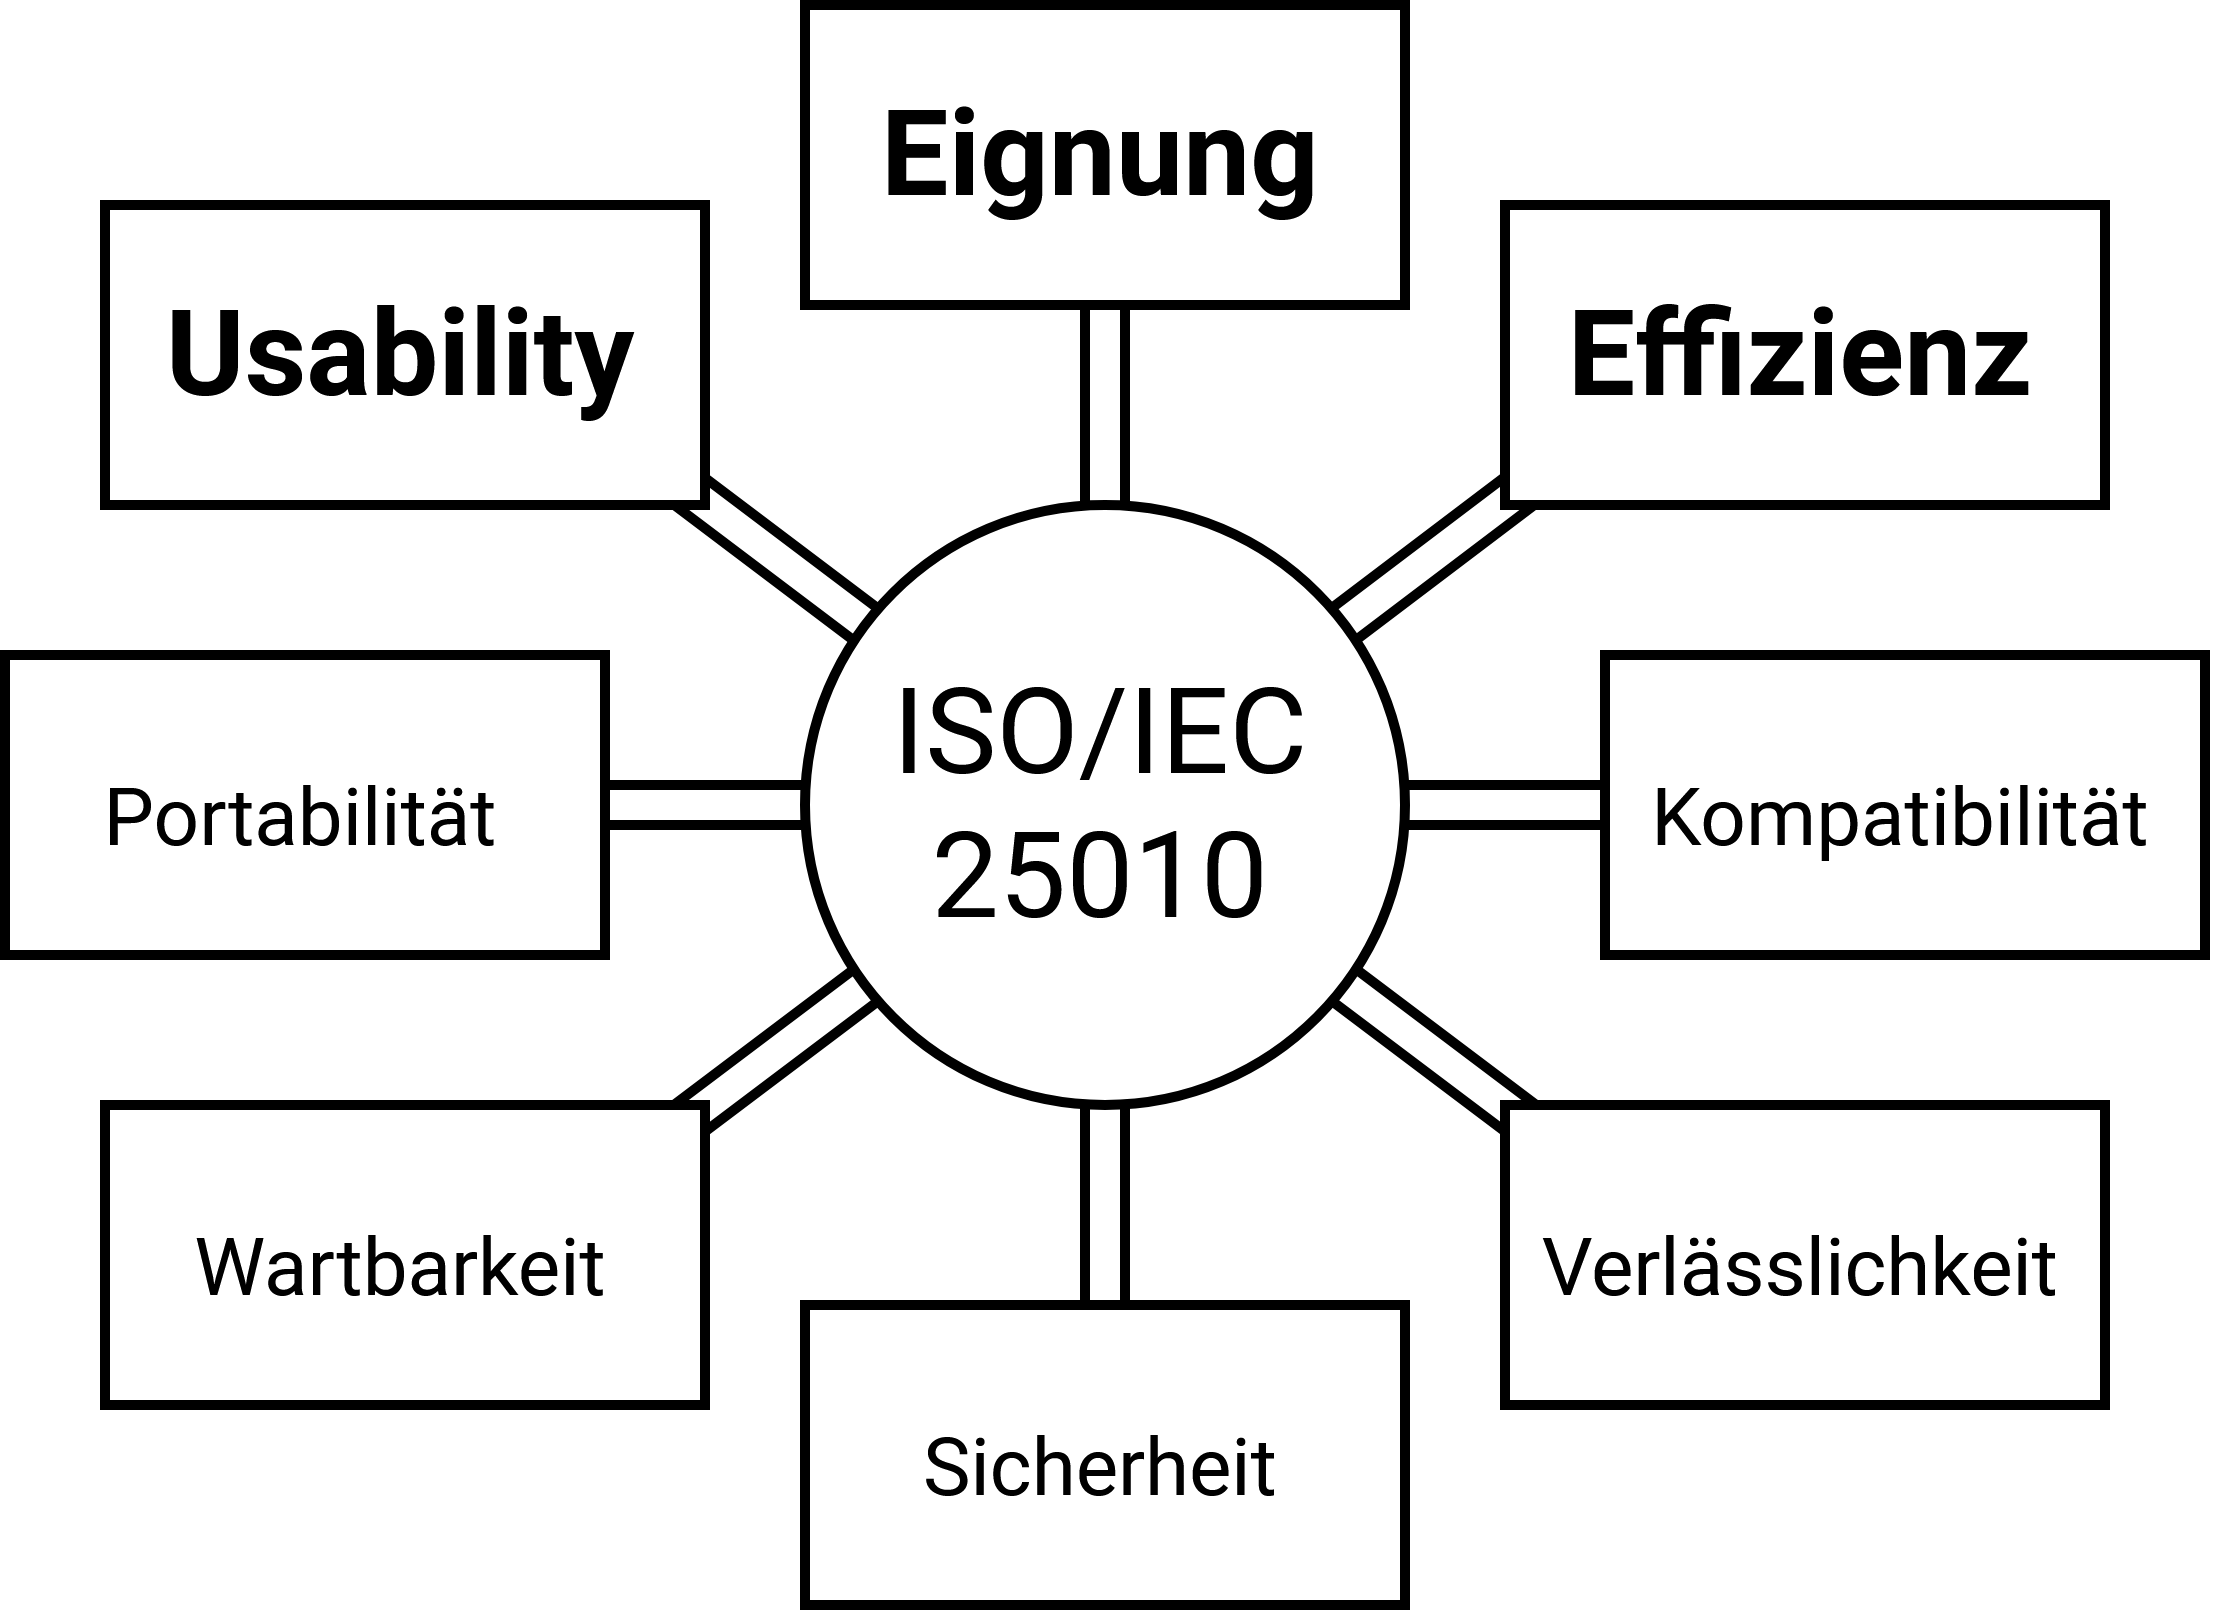
\includegraphics[width=0.8\textwidth]{SoftwareQuality2.png}
\end{figure}

\subsubsection{Benutzerfreundlichkeit}
Die Benutzerfreundlichkeit wird nach ISO/IEC 25010 in sechs Kriterien aufgeteilt: angemessene Erkennbarkeit, Erlernbarkeit, Bedienbarkeit, Toleranz gegenüber Anwenderfehlern, Ästhetik der Benutzeroberfläche und Barrierefreiheit \cite[S.~4]{ISO25010}.

\paragraph{Usability Heuristics}
Die zehn Usability Heuristics von Nielsen sind grundlegende Richtlinien zur Bewertung der Benutzerfreundlichkeit \cite{Nielsen.1994} und decken die ISO/IEC 25010 Kriterien weitestgehend ab. So gibt es zum Beispiel die folgenden Richtlinien:

\begin{itemize}
    \item Das Design sollte die Sprache der Benutzer sprechen, indem vertraute Wörter, Phrasen und Konzepte, statt interne Fachbegriffe verwendet werden \cite[Regel 2]{Nielsen.1994}.
    \item Das Design sollte konsistent sein und etablierten Standards folgen, sodass Benutzer nicht darüber nachdenken müssen, ob verschiedene Wörter, Situationen oder Aktionen dasselbe bedeuten \cite[Regel 4]{Nielsen.1994}.
\end{itemize}

Beide Richtlinien helfen dabei das ISO/IEC 25010 Kriterium der Erlernbarkeit einzuhalten. Während der Entwicklung können die Richtlinien als Orientierungshilfe dienen, um die Benutzerfreundlichkeit zu verbessern. Eine subjektive Einhaltung dieser ist allerdings unzureichend, um die Benutzerfreundlichkeit zu bewerten. Usability Tests eignen sich hierfür besser.

\paragraph{Usability Tests}
Usability Tests erfordern die Beobachtung von Testpersonen bei der Nutzung des zu prüfenden Produkts, während sie vorab entwickelte Anwendungsszenarien durchspielen. Die Testpersonen sollten potenzielle Benutzer des Produkts repräsentieren.\cite[S.~22]{Dumas.1999} Nach der Durchführung der Tests werden die gesammelten Beobachtungen auf Probleme und Schwachstellen im Produkt ausgewertet. Die Tests können entweder quantitativ oder qualitativ durchgeführt werden. Bei quantitativen Usability Tests werden verschiedene Metriken, wie die Durchführungszeit oder die Rate der erfolgreichen Durchführung von Aufgaben gesammelt. Diese Metriken zeigen im Vergleich zu den Ergebnissen früherer oder zukünftiger Tests, wie sich die Benutzerfreundlichkeit zwischen verschiedenen Versionen entwickelt hat. In qualitativen Usability Tests werden Testpersonen bei der Interaktion mit dem Produkt beobachtet, um Designmerkmale zu identifizieren, die gut oder schlecht zu bedienen sind.\cite{Budiu.2017} Qualitative Tests erfordern einen Moderator, der die Testpersonen durch den Testprozess leitet. Gegebenenfalls gibt es auch weitere Beobachter, die nicht mit den Testpersonen interagieren.\cite{Moran.2019} Für qualitative Tests reicht eine Auswahl an fünf Testpersonen aus, um einen Großteil der Probleme zu finden. Mit einer zunehmenden Menge an Testpersonen sinkt das Return of Investment maßgeblich dadurch, dass immer weniger neue Fehler pro Testperson entdeckt werden.\cite{Nielsen.2012}

\subsubsection{Effizienz}\label{sec:PerformanceBasics}
Die Effizienz einer Anwendung beeinflusst die Benutzerfreundlichkeit und Absprungraten maßgeblich und zeichnet sich unter anderem durch die Dauer der Ladezeiten und die Reaktionsgeschwindigkeit der Benutzeroberfläche aus. Für die Bewertung der Effizienz einer Webanwendung oder Webseite gibt es verschiedene Merkmale. Beim Prototyp wird besonders auf die wahrgenommene Ladezeit, die Lade-Reaktionsfähigkeit und die Smoothness geachtet. 

Unter der wahrgenommenen Ladezeit versteht man wie schnell der Ladevorgang dem Nutzer erscheint \cite[Abschnitt~4]{PerformanceMetrics}. Zur Bestimmung dieser Ladezeit wird gemessen, wann bestimmte \ac{UI}-Elemente angezeigt werden. Der \ac{LCP} ist hierbei der wichtigste Messwert, da mit diesem gemessen wird, wann das größte oder wichtigste Element angezeigt wird \cite{LCP}. Der \ac{FCP} ist ein weiterer erwähnenswerter Messwert, mit dem gemessen wird, wann das erste Element angezeigt wird \cite{FCP}.

Unter der Lade-Reaktionsfähigkeit versteht man wie flüssig auf Interaktionen des Nutzers reagiert wird, während der Ladevorgang noch stattfindet \cite[Abschnitt~4]{PerformanceMetrics}. Gemessen wird die Reaktionsfähigkeit vor allem durch den \ac{FID}. Dieser misst die Verzögerung, die bei der ersten Interaktion des Nutzers auftritt \cite{FID}. Zusätzlich kann auch die \ac{TBT} gemessen werden. Hier wird gemessen wie lange der Hauptthread so stark beschäftigt ist, dass Interaktionen nur verzögert verarbeitet werden können \cite{TBT}.

Mit der Smoothness ist die insgesamte Geschmeidigkeit des Nutzererlebnisses gemeint, also ob Übergänge und Animationen mit einer konsistenten Bildrate gerendert werden und flüssig aussehen \cite[Abschnitt~4]{PerformanceMetrics}. Die Smoothness lässt sich durch die \ac{INP} – die Latenz von Interaktionen – messen \cite{INP}.

\newpage
\section{Anforderungen an den Prototyp}\label{sec:Requirements}
In diesem Kapitel werden die funktionalen und nicht-funktionalen Anforderungen an den Prototyp, sowie die Anforderungen an die Modellerzeugungsmethode vorgestellt.

\subsection{Anforderungen an Modellerzeugung}

Für die Relevanz des Prototyps ist es erheblich, dass es eine einfache Methode gibt, mit der 3D-Gebäudemodelle erzeugt werden können. Hierfür soll eine Methode gefunden werden, die diese Anforderung erfüllt. Eine tiefere Analyse der gewählten Methode sowie ein tieferer Vergleich zwischen verschiedenen Methoden ist unerheblich, da die gewählte Methode nicht die beste sein muss. So soll in dieser Arbeit nur herausgearbeitet werden, dass es eine passende Methode gibt, nicht welche am besten für den Anwendungsfall geeignet ist. Trotzdem soll die Methode möglichst geringe Kosten verursachen. Auch sollte die Methode kein besonderes technisches Know-how erfordern, um sich von klassischer Modellierungssoftware wie Blender abzuheben. Die erzeugten Modelle müssen nicht hundertprozentig genau, aber genau genug sein, um eine gute Übersicht zu ermöglichen.

\subsection{Funktionale Anforderungen}\label{sec:FunctionalRequirements}
Wie bereits im Abschnitt \ref{sec:ResearchQuestion} beschrieben, soll der Prototyp als Webanwendung implementiert werden. So wird mit wenig Aufwand eine Plattformunabhängigkeit ermöglicht. Diese ist nötig, da die Anwendung auf beliebigen Geräten nutzbar sein soll. Insbesondere soll die Anwendung sowohl auf Smartphones als auch auf Desktop Computern genutzt werden können, weshalb der Prototyp außerdem responsiv sein soll.

Die Anwendung lässt sich in drei zentrale Funktionen aufteilen: Übersicht, Steuerung und Verwaltung.

\subsubsection{Übersicht}

In der Übersicht sollen die relevanten Roboterdaten zusammen mit dem Gebäudemodell in einer dreidimensionalen Ansicht abgebildet werden. Da die Roboter in der Lage sind Fahrstuhl zu fahren, soll es die Möglichkeit geben zwischen verschiedenen Stockwerken zu navigieren. Es soll außerdem in Echtzeit angezeigt werden, wo sich die Roboter befinden. In der Darstellung sollen die Roboter dann so wie in der Realität fahren. Auch soll ersichtlich sein, ob und womit die Roboter beschäftigt sind. Falls der Roboter einen Lieferauftrag ausführt, soll das Ziel angezeigt werden. Weitere Daten, die von den Robotern stammen und angezeigt werden sollen, sind die Positionen aller möglichen Ausgabe- und Lieferpunkten, sowie Ladestationen. Auch haben die Roboter festgelegte Pfade, an denen sie sich beim Fahren orientieren. Diese Pfade sollen auch angezeigt werden.

\subsubsection{Steuerung}

In der Steuerung sollen die Roboter beauftragt werden können. So soll es die Möglichkeit geben einen Zielpunkt einzustellen. Auch sollen die Roboter an ihre Ladestation geschickt werden können.

\subsubsection{Verwaltung}

In der Verwaltung sollen sowohl die Roboter als auch die Übersicht selbst verwaltet werden können. Das Ändern der verschiedenen Roboter-Einstellungen soll möglich sein. So soll beispielsweise die eingestellte Ladestation geändert werden können.

Es muss außerdem möglich sein die 3D-Gebäudemodelle zu importieren und diese mit den Roboterdaten zu synchronisieren. So muss es die Möglichkeit geben das importierte 3D-Gebäudemodell und die mit \ac{VSLAM} erzeugte interne Karte der Roboter anzugleichen, damit die Positionen der Roboter in der Übersicht mit der Realität übereinstimmen.

\subsubsection{Benutzer}

Für die Anwendung gibt es drei verschiedene Nutzergruppen: Gäste, Mitarbeiter und Administratoren. Der für den Nutzer verfügbare Funktionsumfang erhöht sich in dieser Reihenfolge. So sollen Gäste nur einen eingeschränkten Zugriff auf die Übersicht haben während Administratoren Zugriff auf alle Funktionen der Übersicht, Steuerung und Verwaltung haben.

Der Wert von Servicerobotern muss insbesondere aus der Sicht von Gästen noch bewiesen werden \cite[S.~429]{Paluch2020}. Deshalb sollen Gäste einen eingeschränkten Zugriff auf die Übersicht der Roboter bekommen, in der sie die Positionen und aktuellen Aufträge sehen können. Mithilfe dieser Transparenz sollen ihnen die Vorteile von Servicerobotern veranschaulicht werden.

Die Mitarbeiter sollen einen vollständigen Zugriff auf die Übersicht und Steuerung bekommen. So werden ihnen alle Funktionen zur Verfügung gestellt, die sie für das Steuern der Roboter brauchen. Auch sollen ihnen in der Übersicht mehr Informationen angezeigt werden. Einen Zugriff auf die Verwaltung der Roboter brauchen die Mitarbeiter nicht.

Auf die Verwaltung sollen nur Administratoren Zugriff haben. Während die Verwaltung der Roboter kontinuierlich genutzt werden sollte, sollte die Verwaltung der Stockwerke hauptsächlich bei der Einrichtung gebraucht werden. So sollte die Karte nur zu Beginn eingerichtet und danach nie wieder verändert werden müssen.

\subsection{Nicht-funktionale Anforderungen}
Lange Ladezeiten während der Nutzung der Anwendung können schnell Frust verursachen. Die Reduktion der Ladezeiten ist deshalb eine zentrale Anforderung an den Prototyp. Normalerweise lassen sich Ladezeiten sowohl auf der Server- als auch auf der Client-Seite verbessern. Der Schwerpunkt dieser Arbeit liegt allerdings im Frontend, weshalb sich Optimierungen auch nur auf die Client-Seite beschränken sollen. Das \ac{BCB} soll entsprechend, unabhängig davon, ob Optimierungspotenzial existiert, nicht verändert werden. Maßnahmen, die sich hier anbieten sind das Verzögern des Ladens nicht essenzieller Ressourcen, sowie die Reduktion des Datenverbrauchs. Eine Reduktion des Datenverbrauchs bietet auch den Vorteil, dass sich Kosten für Nutzer reduzieren, die einen teuren oder begrenzten Datenplan verwenden. Unabhängig von Ladezeiten sollte der Prototyp trotz der aufwändigen Darstellung von 3D-Modellen möglichst performant sein. So soll es beispielsweise beim Navigieren keine Ruckler geben. Hierdurch wird auch die Benutzerfreundlichkeit verbessert. Diese Anforderungen lassen sich unter dem Begriff der Performance zusammenfassen. Die Performance soll anhand des \ac{PLS}, der \ac{LR} und der Smoothness bewertet werden.

Neben einer guten Performance sollte die Anwendung auch eine gute Benutzerfreundlichkeit aufweisen, damit sichergestellt wird, dass sich die Benutzer problemlos zurechtfinden können. Die Benutzerfreundlichkeit soll anhand von Usability Tests bewertet werden.

\newpage
\section{Technische Herausforderungen}
Während der Implementierung des Prototyps sind verschiedene größere technische Herausforderungen entstanden, die gelöst werden mussten. Die Herausforderungen mit den gewählten Lösungsansätzen in diesem Kapitel gruppiert. 

\subsection{3D Modelle von Gebäuden}
Fehlender-Text

\subsection{3D Visualisierung im Web}
Für die dreidimensonale Darstellung im Prototyp wurde \deckgl gewählt.
% TODO Weiter erläutern warum deck.gl
% deck.gl kurz vorstellen (inklusive Layers)

\subsubsection{deck.gl}
Fehlender-Text

\subsubsection{Auswahl des Dateiformats der 3D-Modelle}

Für die Darstellung des 3D-Modells gibt es verschiedene Möglichkeiten. Zwei dieser Möglichkeiten sind das Einbinden des \ac{OBJ} Formats in der SimpleMeshLayer von \deckgl und das Einbinden des \ac{glTF} Dateiformats in der ScreengraphLayer. Beide Dateiformate werden in der Scaniverse App als Dateiexport angeboten. Beim \ac{OBJ} Format gibt es das Problem, dass das 3D-Modell mit \deckgl nur ohne Textur dargestellt werden kann. Das \ac{OBJ} Format besteht aus einer Datei mit der Endung \obj in der die dereidimensionalen geometrischen Formen kodiert sind und einer Datei mit der Endung \mtl in der die optische Materialeigenschaften und Texturierung kodiert sind. Die Materialdatei lässt sich nicht in \deckgl einbinden, da die \loadersgl Programmbibliothek nur das Parsen der \obj Datei ermöglicht. Das \ac{glTF} Format besteht im Gegensatz zu \ac{OBJ} nur aus einer Datei mit der Endung \gltf oder \glb, die auch die Materialeigenschaften und Texturierung enthält. Die Ersteller des Dateiformats beschreiben es als "JPEG of 3D", da es eine geringere Dateigröße bietet. Mithilfe der \loadersgl Programmbibliothek lassen sich 3D-Modelle des Dateiformats ohne großen Aufwand in der ScenegraphLayer von \deckgl einbinden. Da ein 3D-Modell mit einer passenden Texturierung eine bessere Übersichtlichkeit bietet und da \ac{glTF} Dateien eine geringe Dateigröße haben, wird im Rahmen des Prototyps weiter mit dem Dateityp und der ScenegraphLayer gearbeitet.

\subsection{Synchronisierung des Gebäudemodells und der Roboterdaten}
Im Prototyp sollen die Roboterdaten in den 3D-Modellen integriert dargestellt werden. Die Roboterdaten und 3D-Modelle haben den gleichen Maßstab, die Positionen und Rotationen der Datensätze stimmen allerdings nicht miteinander überein. Der Grund hierfür ist, dass zur Generierung der Datensätze unterschiedliche Scanning-Methoden eingesetzt werden. Auch die Positionen der 3D-Modelle stimmen nicht miteinander überein, da beim Scannen an verschiedenen Ausganspunkten angefangen wurde.

Aus diesem Grund müssen die Positionen der Roboterdaten mit den 3D-Modellen synchronisiert werden. Auch müssen die Positionen der 3D-Modelle unterienander synchronisiert werden. Eine automatische Synchronisierung ist aus verschiedene Gründen zu komplex. Zum einen sind die Formate der Daten zu verschieden, denn während die 3D-Modelle aus komplexen dreidimensonalen Formen bestehen, setzen sich die Roboterdaten aus zweidimensonalen Linien und Punkten zusammen. Zum anderen gibt es in beiden Datensätzen unterschiedliche Ungenaugkeiten in Bezug auf die Realität. Sowohl \ac{VSLAM}, mit dem die Roboterdaten untereinander positioniert werden, \ac{LiDAR}-Scanning, mit dem die 3D-Modelle für den Prototyp generiert wurden, sind fehlerbehaftet. Da sich diese Scanning-Methoden unterscheiden und somit verschiedene Stärken und Schwächen beim Scannen haben, sind die Ungenauigkeiten zwischen den Roboterdaten und 3D-Modellen größer, während die Ungenauigkeiten zwischen den verschiedenen 3D-Modellen geringer sind.

Da eine automatische Synchronisierung der Datensätze ausgeschlossen ist, muss diese manuell vorgenommen werden. Hierfür wurde ein Editor implementiert, mit dem der Administrator die 3D-Modelle und Roboterdaten durch Verschieben und Rotieren der 3D-Modelle synchronisieren kann. Die Implementierung dieses Editors wird im folgenden Kapitel beschrieben.

% TODO textcommand für Scenegraph-Ebene, SimpleMesh-Ebene, Icon-Ebene

\newpage
\section{Umsetzung des Prototyps}\label{sec:RealizationOfPrototype}
Im Folgenden wird das \gls{Mockup}, die Implementierung und das Deployment des Prototyps beschrieben. Während der Skizzierung der \gls{Mockup}s und der Implementierung wurde auf eine gute Benutzerfreundlichkeit geachtet. Hierfür wurde sich unter anderem an Nielsens Usability Heuristics \cite{Nielsen.1994} orientiert. Im Abschnitt \ref{sec:UsabilityHeuristics} wird genauer geprüft, wie gut diese eingehalten wurden.

\subsection{Mockup}\label{sec:Mockup}
Für den Prototyp wurden \gls{Mockup}s skizziert die während der Implementierung als Orientierungshilfe genutzt wurden. Diese \gls{Mockup}s wurden zunächst auf Papier niedergeschrieben und für die folgende Beschreibung mithilfe von Figma \cite{Figma} digitalisiert. Es gibt jeweils ein \gls{Mockup} für die Übersicht, Steuerung und Verwaltung, sowie für das Routenplanungs-Popup in der Steuerung. Für den Editiermodus wurde kein \gls{Mockup} entworfen, da das Design und Verhalten zu stark von den Möglichkeiten in \deckgl{} abhängt, die noch nicht vollständig bekannt waren, als die \gls{Mockup}s entworfen wurden. Stattdessen wurde das Design und Verhalten des Editiermodus während der Implementierung festgelegt.

Die Abbildung \ref{fig:MockupOverview} im Anhang zeigt das \gls{Mockup} für die Übersicht. In der Übersicht werden die Raummodelle zusammen mit den verschiedenen Roboterdaten angezeigt. So werden die Standorte mithilfe von Icons, die Roboterpfade mithilfe von Linien und die Roboterpositionen mithilfe von 3D-Modellen der Roboter dargestellt. Es gibt außerdem Buttons mit denen zwischen den verschiedenen Stockwerken navigiert werden kann und mit denen die Roboter ausgewählt werden können. Zusätzlich gibt es einen Button, der es ermöglicht den ausgewählten Roboter automatisch zu verfolgen und einen anderen Button, mit dem die Kameraposition wieder zur Ausgangsposition zurückgesetzt werden kann. Die Buttons sind abhängig von ihren Funktionen in den vier Ecken der Anwendung gruppiert.

Die Steuerung erweitert die Übersicht nur um weitere Funktionen und unterscheidet sich daher kaum von dieser. Abbildung \ref{fig:MockupControls} im Anhang zeigt das \gls{Mockup} der Steuerung. Der einzige Unterschied zur Übersicht sind die zusätzlichen Buttons mit denen eine Lieferroute bestimmt, der Roboter zum Aufladen geschickt und der aktuelle Lieferauftrag abgebrochen werden kann. Die Abbildung \ref{fig:MockupRoutePlanner} im Anhang zeigt das \gls{Mockup} für das Routenplanungs-Popup das sich öffnet, wenn der Lieferroute-Button ausgewählt wird. In dem Popup muss ein Ziel und ein Roboter ausgewählt werden, bevor der Auftrag gestartet werden kann. Um die Routenerstellung zu vereinfachen, sollen sowohl Roboter als auch Standorte zusätzlich über das Anklicken auf der Karte auswählbar sein.

Die Abbildung \ref{fig:MockupAdministration} zeigt das \gls{Mockup} für die Verwaltung. Hier gibt es jeweils eine Liste für die Roboter und die Stockwerke. In der Liste der Roboter können verschiedene Informationen der einzelnen Roboter, wie beispielsweise der systeminterne \ac{ID} und die tägliche Neustartzeit ausgelesen werden. Auch können Einstellungen der Roboter, wie Name und Ausgabepunkt geändert werden. Zudem gibt es für jeden Roboter eine Vorschau der Übersicht, in der die Position des Roboters gezeigt wird. Sowohl in der Liste der Roboter als auch in der Liste der Stockwerke gibt es für jedes Stockwerk eine Auflistung der Standorte. In der Liste der Stockwerke gibt es außerdem eine Vorschau der Übersicht und zusätzlich ein Kontextmenü, über das in den Editiermodus des Stockwerks gewechselt werden kann.

\subsection{Implementierung}
Es wurde ein Frontend entwickelt, dass auf das \ac{BCB} zugreift, um die Roboterdaten anzufragen. Wie das \ac{BCB} hierbei mit den Robotern kommuniziert, wird im Abschnitt \ref{sec:BotControlBackend} erklärt. Das Frontend nutzt das Web-Framework React mit \ac{HTML}, \ac{Sass} und TypeScript. Die Vorteile von TypeScript und \ac{Sass} gegenüber JavaScript und \ac{CSS}, wie auch das Web-Framework React werden im Abschnitt \ref{sec:WebTechnologies} genauer erläutert. Zustandsinformationen die React-Komponenten übergreifend abgerufen werden, werden zentral mithilfe von Redux gespeichert. Die Grundstruktur des Frontend-Projekts wurde mithilfe des Shell Befehls npx create-chayns-app \cite{CreateChaynsApp} aufgesetzt. Die Kompilierung ist mithilfe des \ac{npm}-Pakets chayns-toolkit \cite{ChaynsToolkit} konfiguriert. \ac{GUI}-Elemente wie Buttons und Aufklapper werden durch die Komponentenbibliothek chayns-components \cite{ChaynsComponents} bereitgestellt. Außerdem werden die \ac{npm}-Pakete clsx \cite{clsx} und fortawesome \cite{fontawesome} genutzt. Mithilfe von clsx lassen sich \ac{HTML}-Klassennamen dynamisch anwenden. Das fortawesome \ac{npm}-Paket wird genutzt, um \ac{SVG} Icons als Zeichenkette zu importieren.

\subsubsection{Übersicht}
In der Übersicht werden die Roboterdaten in Kombination mit den Gebäudemodellen mithilfe von \deckgl{} angezeigt. Hierfür werden verschiedene Ebenen eingesetzt. Auch bietet die Übersicht eine Echtzeitaktualisierung der Roboter und Interaktivität für den Nutzer.

\paragraph{Gebäudemodelle}
Für den Prototyp sind die \ac{URL}-Verweise der 3D-Modelle hartkodiert, oder in anderen Worten in den Quelltext der Webanwendung eingebettet. Für ein potenzielles Produktivsystem müssten die \ac{URL}-Verweise in der Datenbank des \ac{BCB}s abgespeichert werden. Die Modelle sind im chayns.space gespeichert, nutzen – aus Gründen, die im Abschnitt \ref{sec:ModelFileFormat} erläutert werden – das \ac{glTF}-Format und werden über die ScenegraphLayer angezeigt. Diese Ebene ist dafür ausgelegt, ein bestimmtes 3D-Modell beliebig oft an verschiedenen Positionen anzuzeigen \cite{DeckglScenegraphLayer}, was auf die Hauptfunktion von \deckgl{} – die Visualisierung riesiger Geodaten Mengen \cite[S.~3]{YangWang2019} – zurückzuführen ist. Unterschiedliche 3D-Modelle lassen sich nicht in einer ScenegraphLayer-Instanz einbinden, weshalb für jedes 3D-Modell eine eigene Instanz der ScenegraphLayer erzeugt werden muss. \deckgl{} ist für den Einsatz von über 100 Ebenen gleichzeitig ausgelegt, wobei wahrscheinlich sogar der Einsatz von bis zu 1000 Ebenen ohne große Performance Einbußen möglich ist \cite{DeckglPerformance}. Im Prototyp besteht ein Stockwerk aus bis zu sechs 3D-Modellen und somit auch aus bis zu sechs ScenegraphLayers, wehalb davon auszugehen ist, dass nie mehr als 100 Modelle für die Darstellung eines Stockwerks erforderlich sind. In Anbetracht dessen, dass nie mehrere Stockwerke gleichzeitig angezeigt werden, ist es unwahrscheinlich, dass die beschriebene mehrfache Verwendung der Ebene negative Auswirkungen auf die Performance hat. Für die Ebenen ist das Backface Culling aktiviert. Mithilfe vom Backface Culling werden die von der Kamera weg gerichteten Polygone ausgeblendet \cite{BackfaceCulling}. Meist wird Backface Culling genutzt, um Polygone auszublenden, die sowieso hinter anderen Polygonen versteckt sind, wodurch die Darstellungsgeschwindigkeit erhöht wird. Im Fall der Gebäudemodelle sind die Polygone in den Raum hineingerichtet. Somit bewirkt das Backface Culling, dass die Wände und Decken, die dem Nutzer die Sicht in den Raum verdecken, ausgeblendet werden. In der Abbildung \ref{fig:BackfaceCulling} wird dieser Effekt deutlich. So sieht man auf der linken Seite, dass ohne das Backface Culling nicht von außen in den Raum hineingesehen werden kann, während es auf der rechten Seite mit aktiviertem Backface Culling möglich ist.

\begin{figure}[H]
    \caption{Raummodell ohne und mit Backface Culling}\label{fig:BackfaceCulling}
    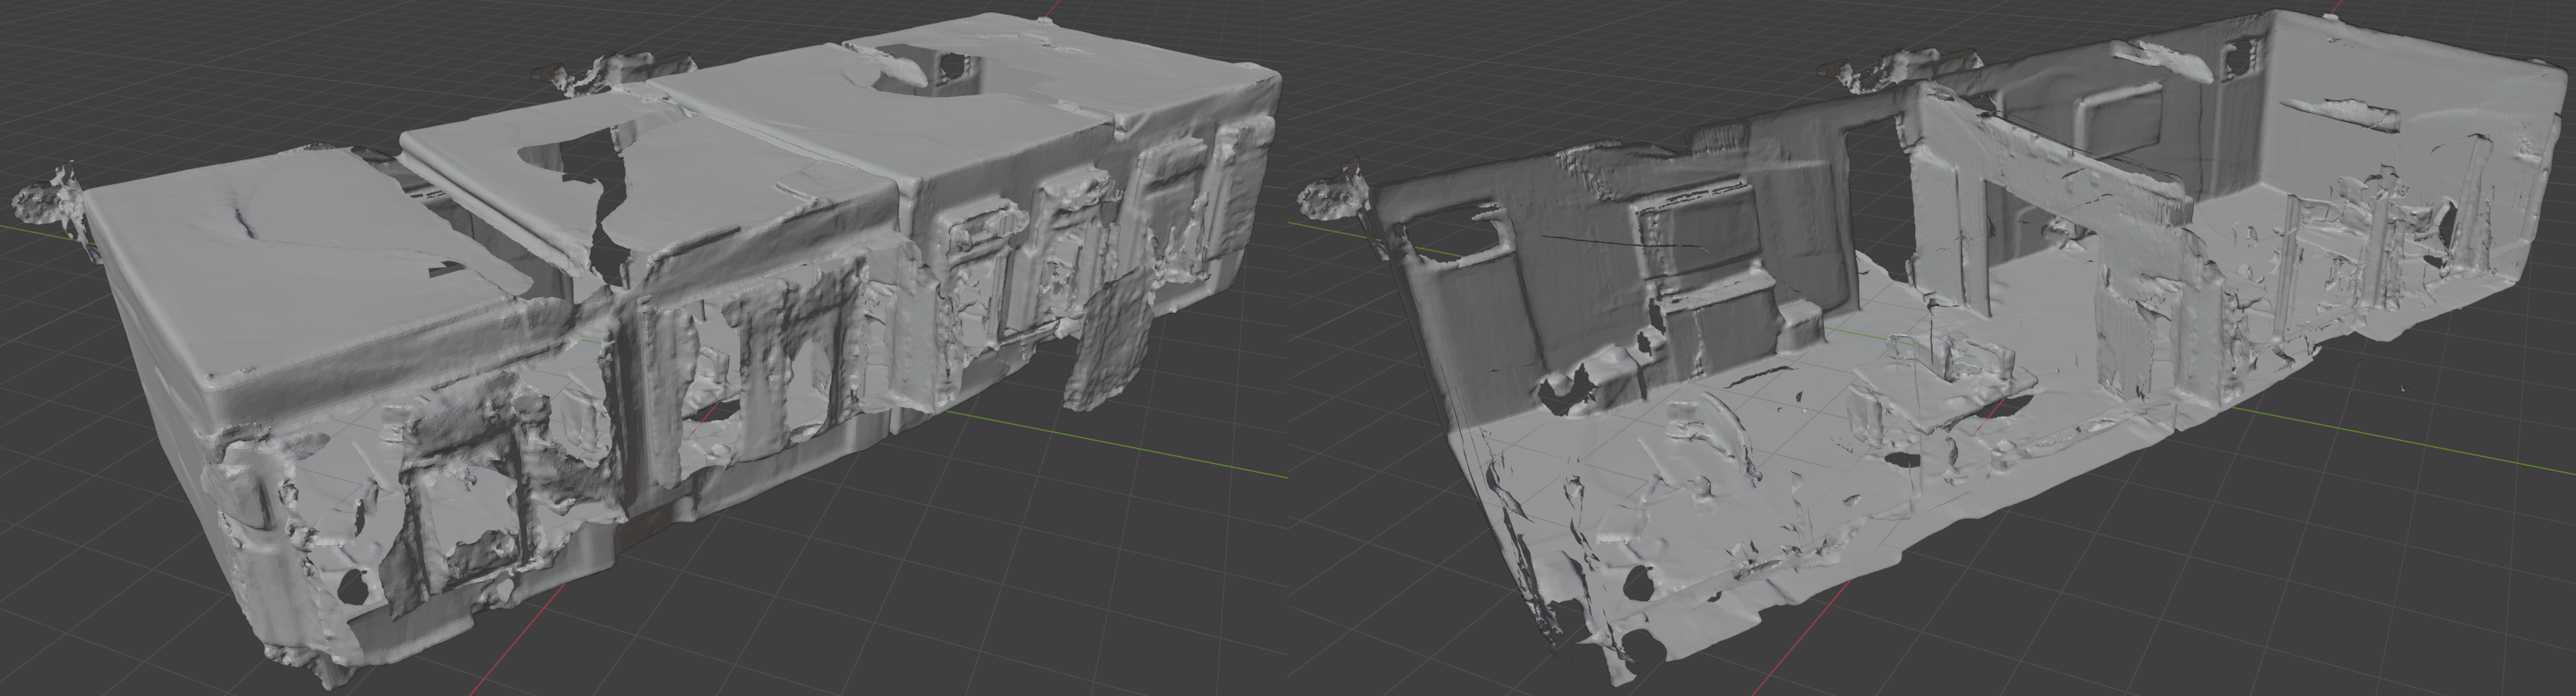
\includegraphics[width=0.9\textwidth]{Backface Culling Vergleich.png}
    \\
    Quelle: Eigene Darstellung
\end{figure}

\paragraph{Roboterdaten}\label{sec:RobotData}
Die Roboterdaten werden über verschiedene Endpunkte des \ac{BCB}s abgerufen. So gibt es einen Endpunkt für die Bezeichnungen der verschiedenen Standorte und einen Endpunkt für den Roboterstatus, Lieferauftrag und die Roboterposition \cite{BCBSwagger}. Für die Positionen aller Standorte und Roboterpfade gibt es keinen Endpunkt. Stattdessen können die Standorte und Pfade nur von Stockwerken angefragt werden, in denen sich zu dem Zeitpunkt Roboter befinden. Damit immer alle Daten aus allen Stockwerken abgerufen werden können, sind diese Daten im Prototyp für alle Stockwerke hartkodiert. Für ein potenzielles Produktivsystem müssten diese Daten in der Datenbank des \ac{BCB}s gespeichert und regelmäßig mit den Robotern synchronisiert werden.

Im Gegensatz zu den Gebäuademodellen werden die Robotermodelle im \ac{OBJ}-Format mit der SimpleMeshLayer \cite{DeckglSimpleMeshLayer} angezeigt. Mit der ScenegraphLayer gibt es das Problem, dass die Positionsänderungen der Modelle nicht animiert werden können, wodurch die SimpleMeshLayer brauchbarer, aber auch nicht ideal, ist. Laut der Dokumentation von \deckgl{} sollte das Animieren über die transition Property in allen Ebenen möglich sein \cite{DeckglLayerClass}. Deshalb handelt es sich bei dem Problem mit der ScenegraphLayer vermutlich um einen Bug. Wie im Abschnitt \ref{sec:ModelFileFormat} erwähnt, lässt sich die Materialdatei des \ac{OBJ} Formats nicht in der SimpleMeshLayer einbinden, weshalb die Roboter einfarbig angezeigt werden müssen. Das ist nicht unbedingt ein Nachteil, denn so können die Roboter durch eine herausstechende Farbe für den Nutzer besser sichtbar gemacht werden. Die Positionsänderungen der Roboter werden über die transitions Property animiert \cite{DeckglLayerClass}. Allerdings lässt sich die Rotationsänderungen nicht animieren, was vermutlich auch auf einin \deckgl{} zurückzuführen ist.

Über den Robotermodellen wird mithilfe der IconLayer der aktuelle Status der Roboter angezeigt. Während in einer ScenegraphLayer-Instanz nur ein bestimmtes 3D-Modell angezeigt werden kann, können in einer IconLayer-Instanz mithilfe der getIcon Zugriffsfunktion verschiedene Bilder angezeigt werden \cite{DeckglIconLayer}. So reicht im Gegensatz zur ScenegraphLayer eine IconLayer-Instanz aus, um alle Icons anzuzeigen. Die genutzten Icons stammen aus der Icon-Bibliothek Fontawesome und werden aus dem fortawesome \ac{npm}-Paket als \ac{SVG}-Zeichenkette importiert. Da die IconLayer \ac{SVG}-Zeichenketten nicht unterstützt, werden diese in das Data-\ac{URL} Format umgewandelt. Das Data-\ac{URL} Format kann Daten als \gls{Base64}-Zeichenkette innerhalb einer \ac{URL} einbetten \cite{DataUrlSpec}, was von der SimpleMeshLayer ausgelesen werden kann \cite{DeckglIconLayer}.

Die verschiedenen Standorte werden über eine weitere IconLayer-Instanz angezeigt. Wie bei den Roboter-Zuständen werden hierfür verschiedene Fontawesome-Icons genutzt. Wurde ein Roboter ausgewählt und hat dieser einen Lieferauftrag, dann wird der Zielstandort farbig markiert. Die Pfade und virtuellen Wände werden über eine Instanz der PathLayer \cite{DeckglPathLayer} dargestellt. Die virtuellen Wände werden gestrichelt und in einer anderen Farbe angezeigt, damit diese von den Roboterpfaden unterschieden werden können. Für die gestrichelte Darstellung wird die PathStyleExtension \cite{DeckglPathStyleExtension} genutzt. Der Boden der 3D-Modelle liegt relativ konstant auf der z-Koordinate – der vertikalen Position – 0. Aufgrund der Ungenauigkeiten die durch den \ac{LiDAR}-Scan entstehen ist der Boden der 3D-Modelle nicht vollständig eben. Da die Positionen der Roboterdaten zweidimensional sind, und somit keine vertikale Position haben, besteht die Gefahr, dass diese an manchen Stellen unter dem Boden der 3D-Modelle verschwinden, wenn sie auf der z-Koordinate 0 angezeigt werden. Aus diesem Grund werden die Icons und Pfade an einer leicht erhöhten z-Koordinate positioniert.

Zusammenfassend wird für die Kartendarstellung die ScenegraphLayer, PathLayer, IconLayer und SimpleMeshLayer genutzt. In Abbildung \ref{fig:MapSchematic} wird dargestellt wie sich die Kartendarstellung aus den einzelnen Ebenen zusammensetzt. Bei der ScenegraphLayer muss beachtet werden, dass für jedes 3D-Modell eine eigene Instanz erstellt wird. Ansonsten stimmt die Menge der Ebenen-Instanzen mit denen im Schaubild überein.

\begin{figure}[H]
    \caption{Kartendarstellung}\label{fig:MapSchematic}
    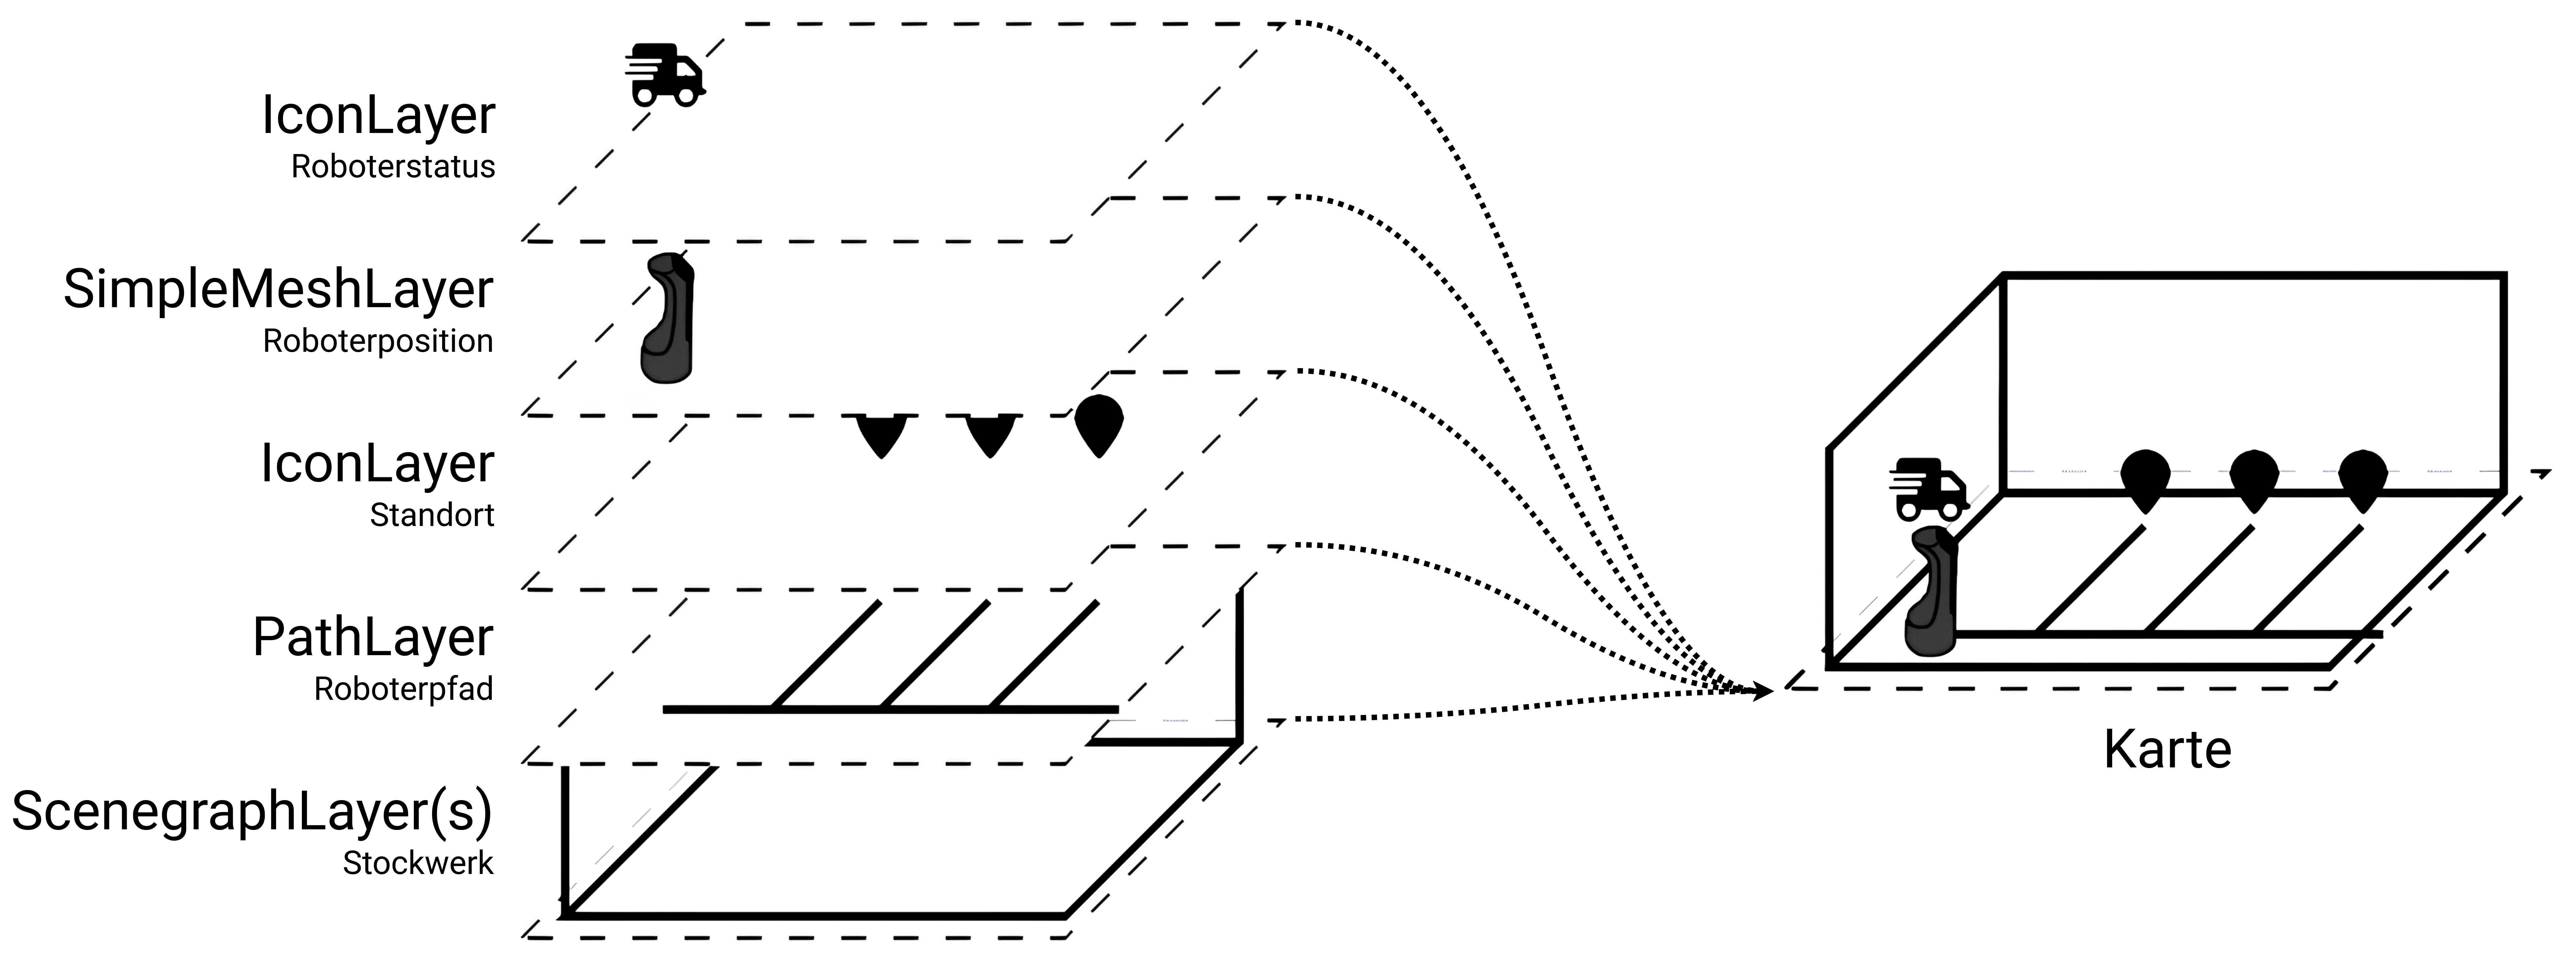
\includegraphics[width=0.9\textwidth]{Layers Schaubild.png}
    \\
    Quelle: In Anlehnung an OpenJS Foundation \cite{DeckglBaseMaps}
\end{figure}

Bei der Abbildung \ref{fig:OverviewScreenshot} handelt es sich um einen Screenshot aus der Übersicht im Prototyp. Man sieht alle erwähnten Ebenen, sowie die verschiedenen Buttons. Basierend auf dem Feedback aus den Usability Tests, die im Abschnitt \ref{sec:UsabilityTests} genauer beschrieben werden, wurden Buttons ergänzt, die es nicht im \gls{Mockup} gibt.

\begin{figure}[H]
    \caption{Übersicht}\label{fig:OverviewScreenshot}
    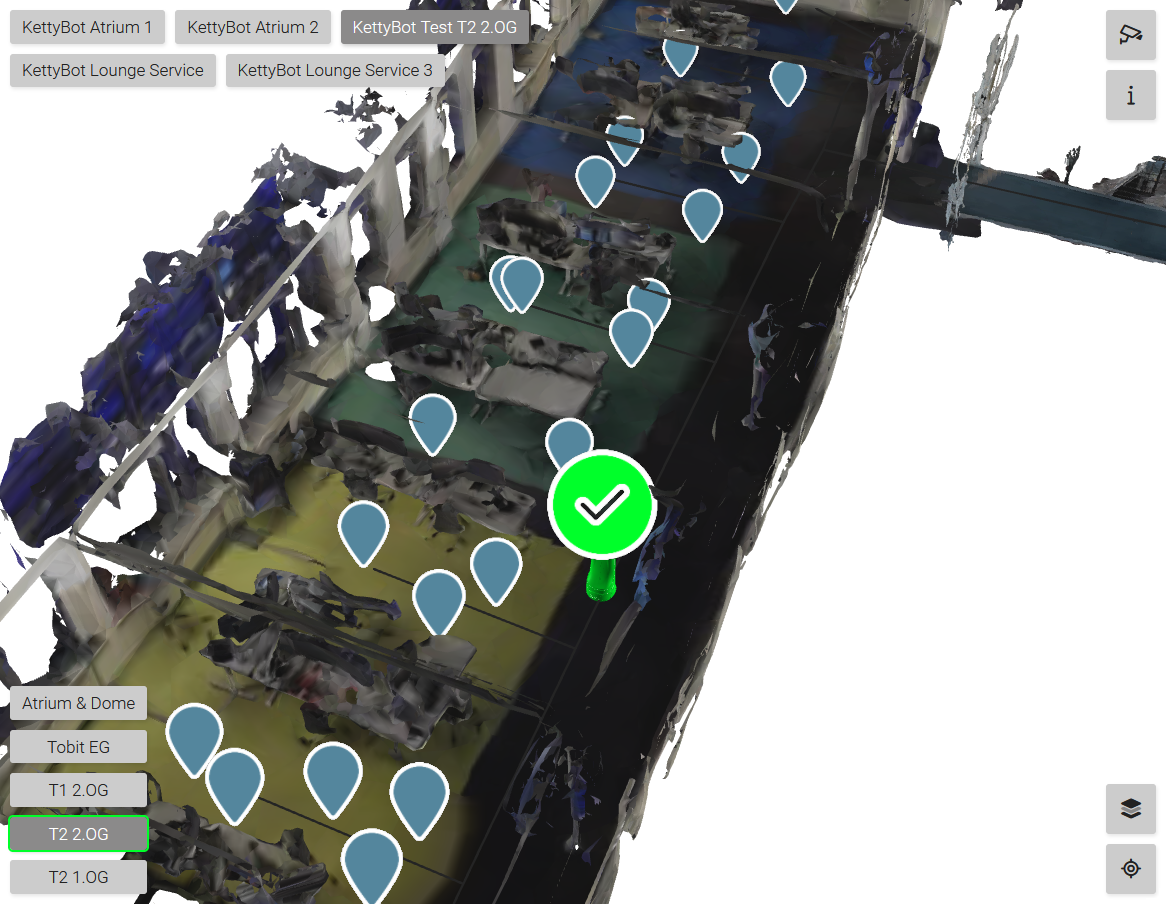
\includegraphics[width=0.9\textwidth]{Screenshot Uebersicht.png}
    \\
    Quelle: Eigene Darstellung
\end{figure}

\paragraph{Echtzeit-Aktualisierung}
Die Positionen sowie weitere Statusinformationen der Roboter, wie beispielsweise der aktuelle Auftrag und Akkuladung, werden mithilfe einer indirekten Verbindung zwischen der Webanwendung und dem \ac{BCB} regelmäßig aktualisiert. Hierfür wird der im Abschnitt \ref{sec:Chayns} erwähnte \gls{Websocket}-Service genutzt. In der Abbildung \ref{fig:RobotStatusUpdate} ist der Ablauf einer Statusaktualisierung vereinfacht dargestellt. Aktualisiert ein Roboter seine Position, wird die entsprechende Information an das \ac{BCB} gesendet. Wie die Kommunikation zwischen Robotern und \ac{BCB} funktioniert wird im Abschnitt \ref{sec:BotControlBackend} erklärt.
% Passt das so? Funktioniert MQTT wie beschrieben?
Das \ac{BCB} sendet daraufhin eine Nachricht an den \gls{Websocket}-Service, der diese Information wiederum an alle verbundenen Clients schickt, die Nachrichten des \ac{BCB}s erwarten. So sieht man in der Abbildung auch, dass der dritte Client keine Nachricht empfängt, da er Nachrichten eines anderen Systems erwartet.

\begin{figure}[H]
    \centering
    \caption{Kommunikationsweg von Statusaktualisierungen der Roboter}\label{fig:RobotStatusUpdate}
    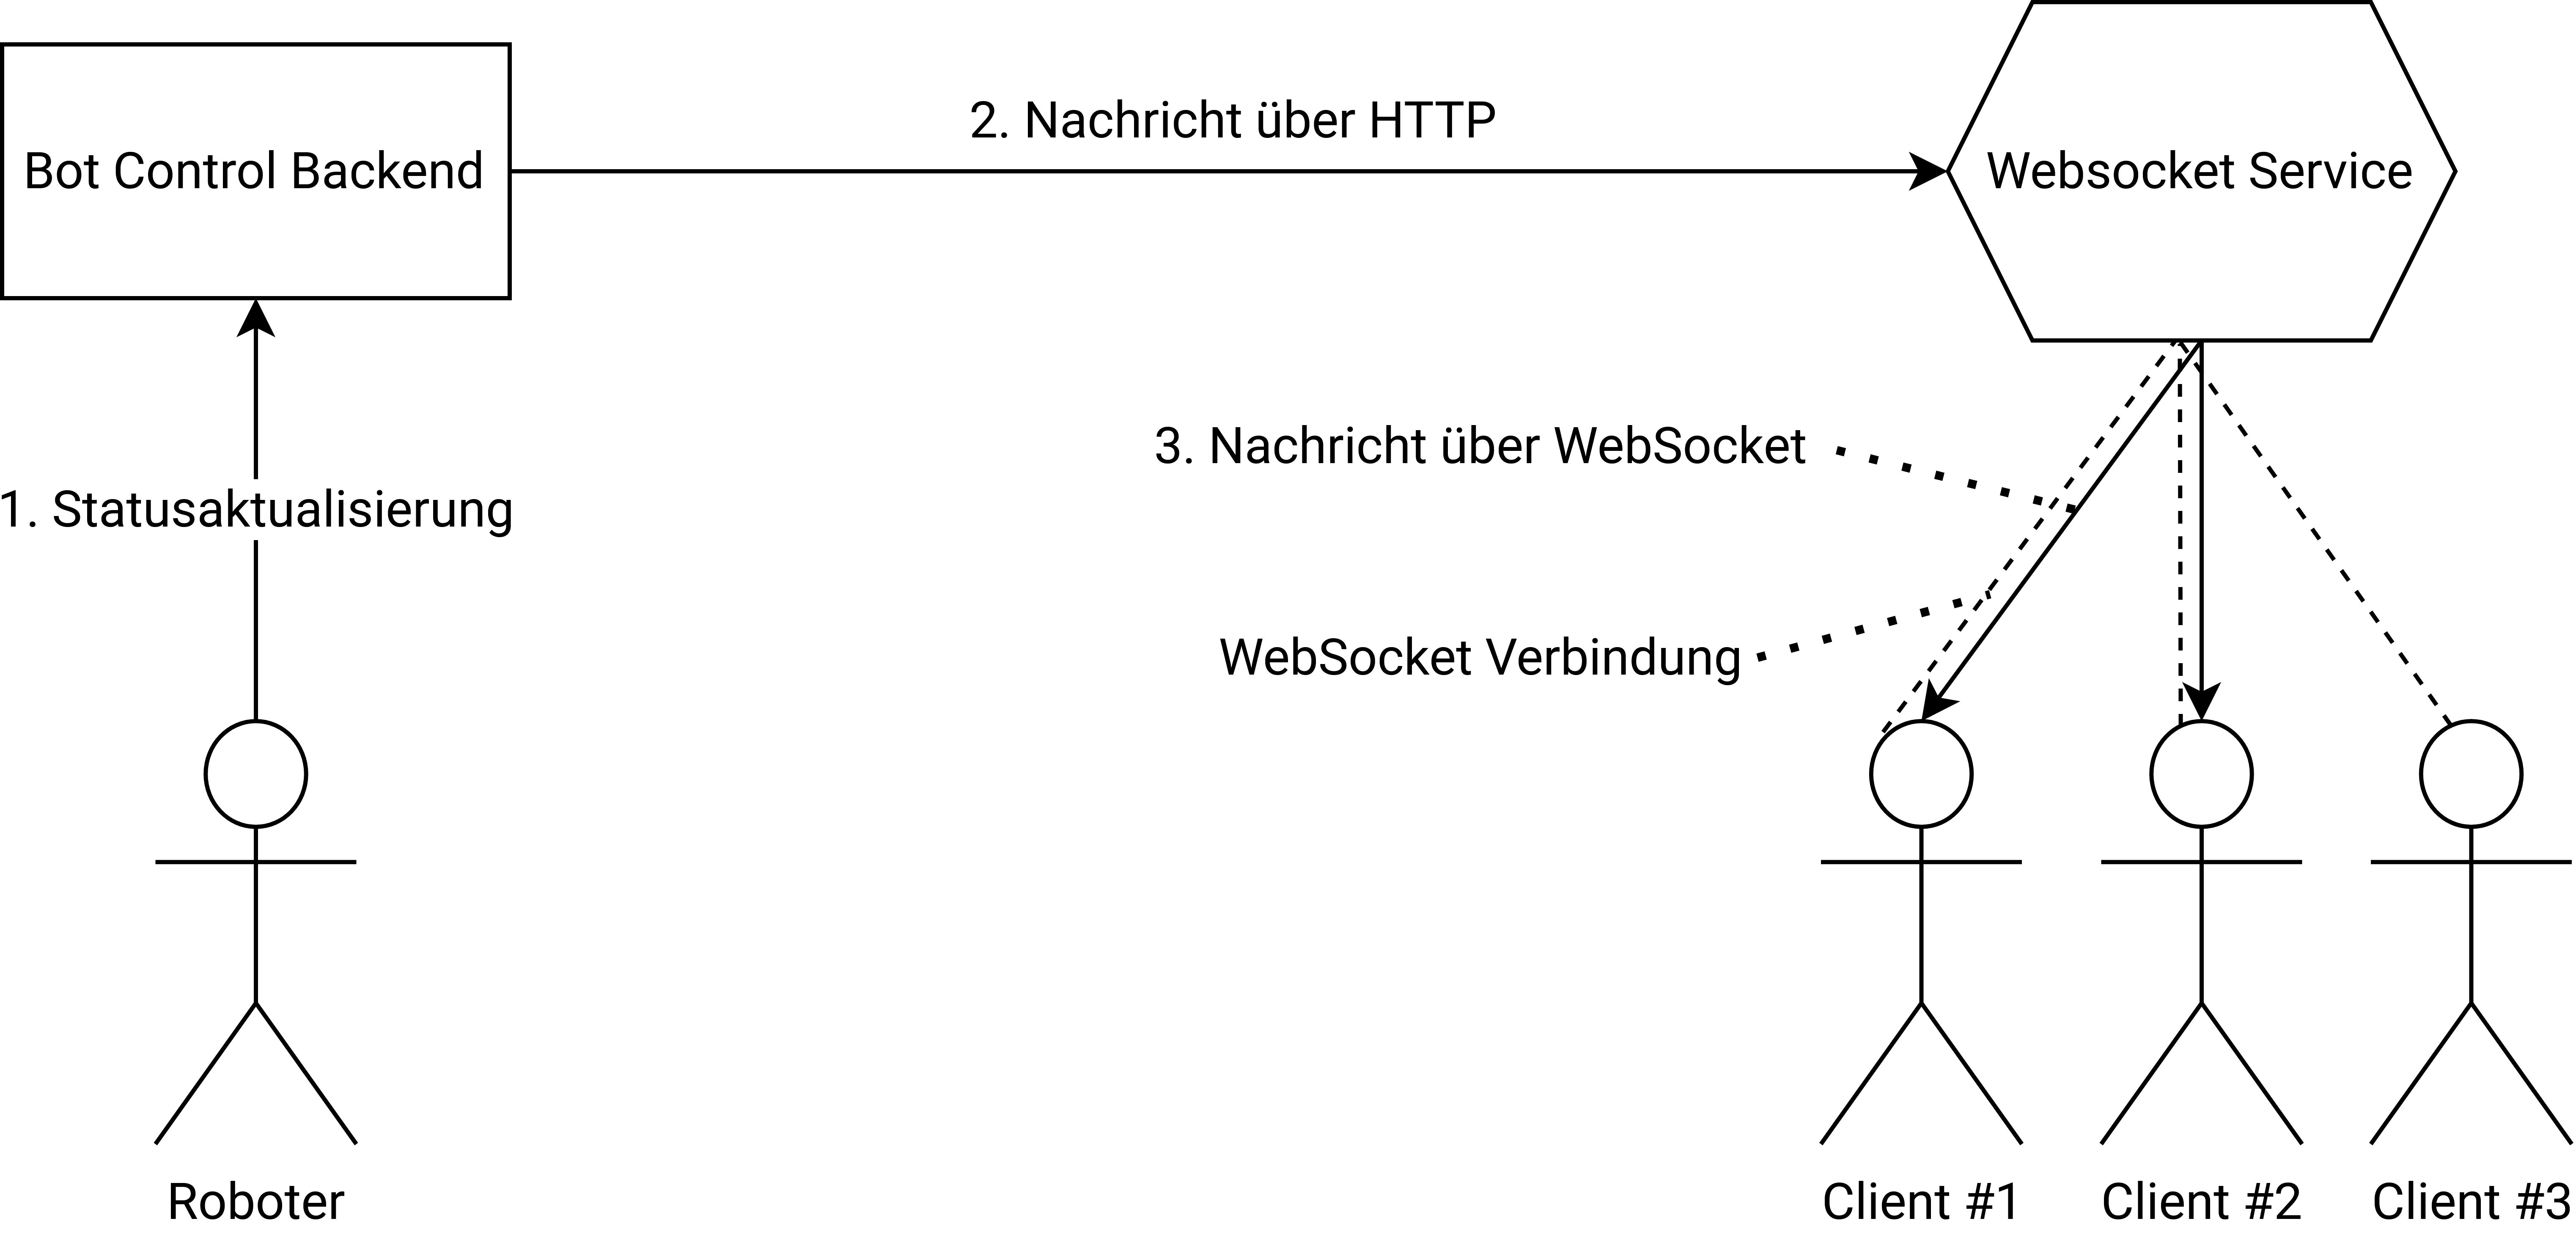
\includegraphics[width=0.9\textwidth]{Websocket Service.png}
    \\
    Quelle: Eigene Darstellung
\end{figure}

Die über den \gls{Websocket}-Service empfangene Statusaktualisierung wird zentral im Redux-Store gespeichert, sodass dem Nutzer direkt die aktualisierten Informationen angezeigt werden können.

\paragraph{Interaktion}
Die Roboter, sowie die Standorte sind mithilfe der onClick Property der entsprechenden Ebene \cite{DeckglInteractivity} auswählbar. Ausgewählte Standorte und Roboter werden verfärbt angezeigt. Außerdem erscheint beim Auswählen eines Roboters ein Button über den sich weitere Informationen wie die Akkuladung anzeigen lassen. Schwebt die Maus über einem Standort oder Roboter, dann wird mithilfe der getTooltip Property \cite{DeckglDeckClass} ein Tooltip angezeigt, in dem der Name des entsprechenden Objekts und weitere wichtige Informationen stehen. Es gibt zudem einen Button, über den einem Roboter gefolgt werden kann. Die Kamera wird hierfür durch den FlyToInterpolator \cite{DeckglFlyToInterpolator} zum ausgewählten Roboter bewegt. Beim Folgen eines Roboters wird die Kameraposition mithilfe der transitionDuration Property \cite{DeckglAnimationsAndTransitions} animiert.

\subsubsection{Steuerung}
Wie im Abschnitt \ref{sec:Mockup} beschrieben, gibt es drei Aktionen die zum Steuern der Roboter ausgeführt werden können: Lieferauftrag, Laden und Abbrechen. Mit dem Laden und Abbrechen wird der aktuelle Lieferauftrag abgebrochen, worauf der Nutzer auch über einen Bestätigungsdialog hingewiesen wird. Für das Starten eines Lieferauftrags muss ein Ziel und ein Roboter angegeben werden. Hierfür gibt es Inputs, mit denen nach Standorten und Robotern gesucht werden kann. Bei den Inputs handelt es sich um die PersonFinder React-Komponente \cite{ChaynsPersonFinder} der chayns-components, die eigentlich für die Suche nach chayns Nutzern genutzt wird, im Prototyp aber für die Suche nach Robotern und Standorten konfiguriert ist. Das Ziel und der Roboter lassen sich außerdem über das Anklicken auf der Karte auswählen. Die Roboter können zudem über ihre Buttons ausgewählt werden. Bestimmte Standorte wie Türen oder Fahrstühle können nicht als Zielstandorte ausgewählt werden. Aus diesem Grund sind diese weder im Input und noch auf der Karte auswählbar. Zum endgültigen Ausführen der drei Aktionen werden die entsprechenden Endpunkte Robot/Call, Robot/Charge und Robot/Cancel im \ac{BCB} \cite{BCBSwagger} aufgerufen. Die Abbildung \ref{fig:ControlsScreenshot} zeigt die Steuerung und das Routenplanungs-Popup. Im Popup sind bereits Ziel und Roboter eingestellt. Der ausgewählte Standort ist auf der Karte farblich markiert.

\begin{figure}[H]
    \caption{Steuerung und Routenplanung}\label{fig:ControlsScreenshot}
    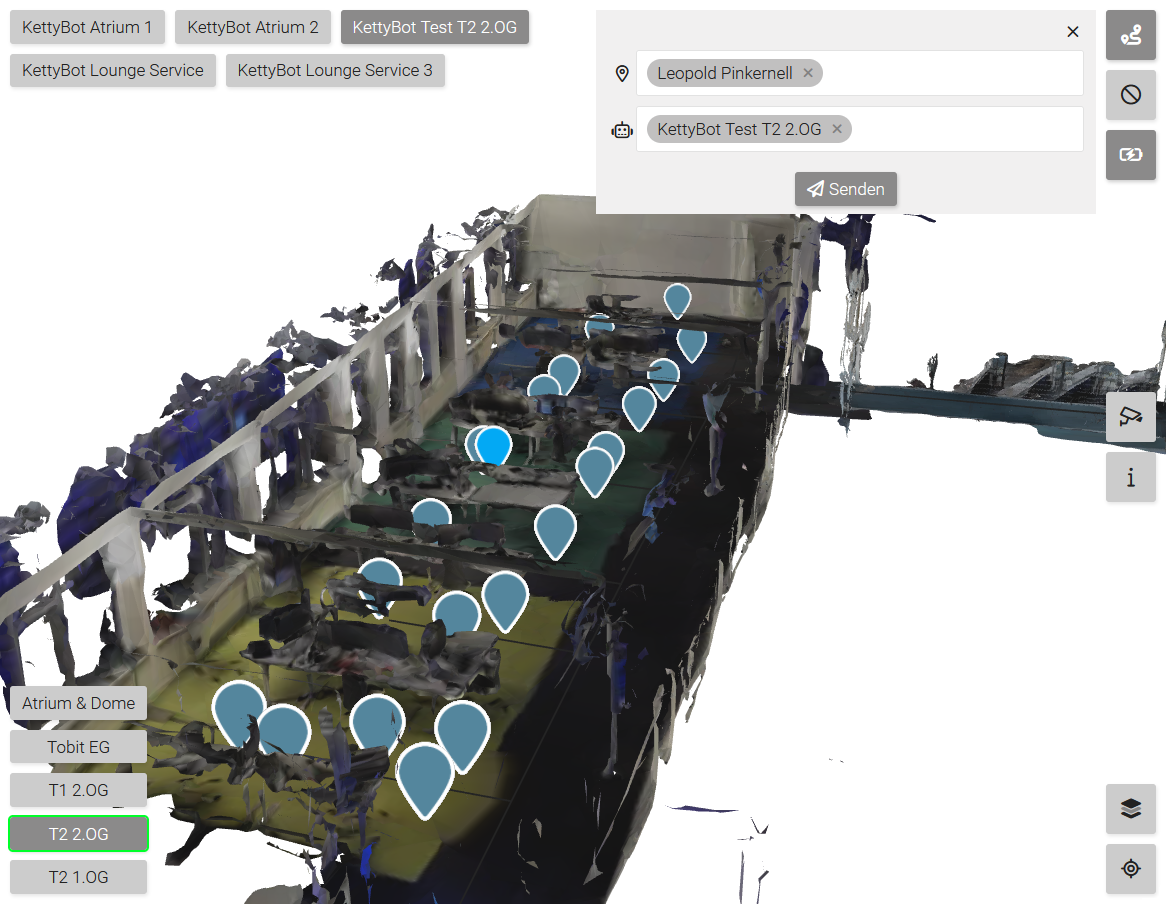
\includegraphics[width=0.9\textwidth]{Screenshot Steuerung.png}
    \\
    Quelle: Eigene Darstellung
\end{figure}

\subsubsection{Verwaltung}
Die Verwaltung ist nicht besonders komplex, da die Daten der Roboter und Stockwerke in jeweils einem Array strukturiert sind und somit leicht mithilfe von React gemappt werden können. Hiermit ist gemeint, dass die Arrays mithilfe der map Funktion zu Arrays an React-Komponenten umgewandelt werden können, die daraufhin gerendert werden können \cite[S.~35-36]{Boduch2020}.

In der Roboterliste werden im Gegensatz zum \gls{Mockup} mehr Statusinformationen angezeigt. Auch können mehr Einstellungen der Roboter geändert werden. Da die Übersicht der verschiedenen Standorte auch über die Liste der Stockwerke ersichtlich ist und dadurch redundant ist, wurde diese aus der Roboterliste entfernt. Bei der Abbildung \ref{fig:RobotlistScreenshot} handelt es sich um einen Screenshot der Verwaltung im Prototyp. Man sieht einen geöffneten Roboter-Eintrag, das Kontextmenü, über das Einstellungen geändert werden können und einen Tooltip, in dem eine Statusinformation erläutert wird.

\begin{figure}[H]
    \caption{Verwaltung}\label{fig:RobotlistScreenshot}
    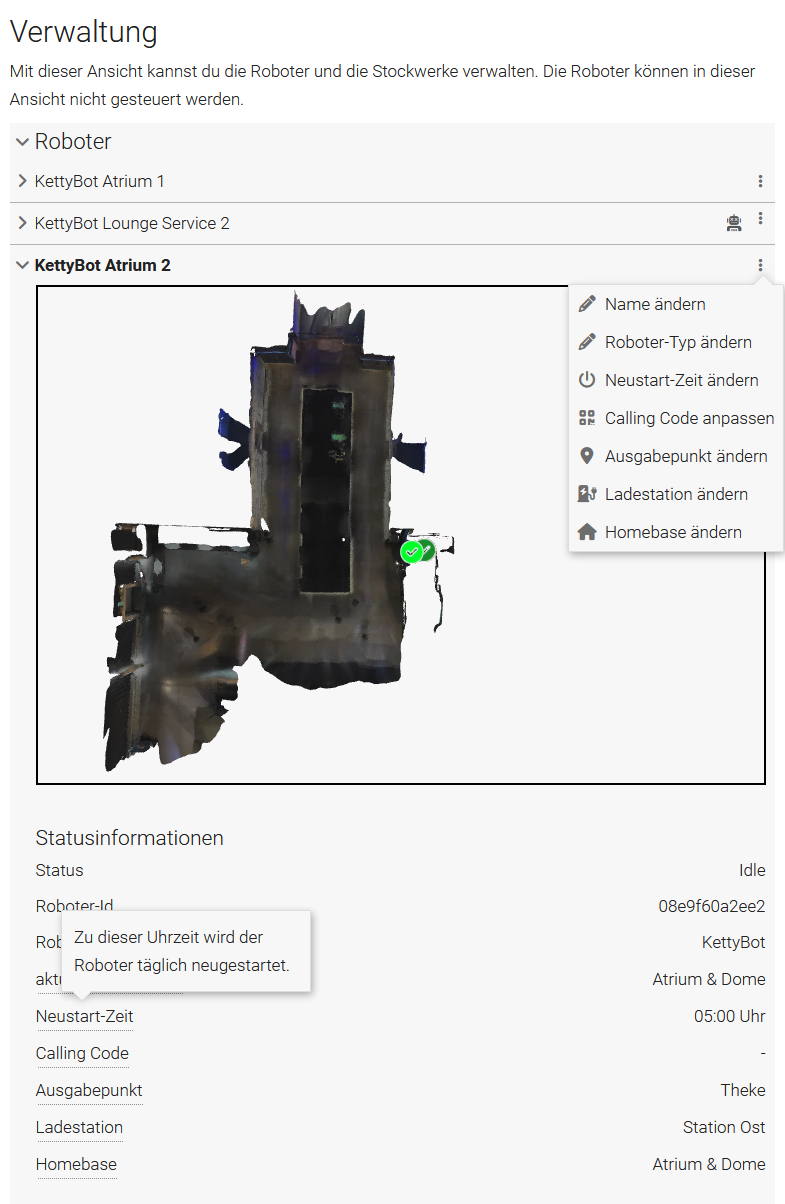
\includegraphics[width=0.6\textwidth]{Screenshot Verwaltung.png}
    \\
    Quelle: Eigene Darstellung
\end{figure}

Die Stockwerkliste unterscheidet sich nur geringfügig vom \gls{Mockup}. So werden die Standorte im Gegensatz zum \gls{Mockup} gruppiert nach der Art des Standorts aufgelistet. Diese Gruppierung ist hilfreich, da die Art des Standortes nicht unbedingt aus dem Namen ersichtlich ist.

Sowohl in der Roboter- als auch in der Stockwerkliste gibt es eine Vorschau des entsprechenden Stockwerks, um die Position des Roboters oder die Positionen der Standorte zu zeigen. Hierbei handelt es sich um die Nutzeransicht mit reduzierten Funktionen. Die Vorschau ist im \gls{Mockup} automatisch geöffnet, was ein Problem ist, da die entsprechende \deckgl{}-Karteninstanz – aufgrund des Verhaltens der genutzten Aufklapper-Komponente – beim Öffnen des Aufklappers initialisiert wird. Die Initialisierung der \deckgl{} Karteninstanz ist rechnerisch aufwändig und verursacht beim ersten Öffnen des Aufklappers starke Ruckler in der Aufklapper-Animation. Um diese Ruckler zu verhindern wird ein Button angezeigt, über den die Karte manuell initialisiert werden kann. Dadurch gibt es die Ruckler beim Klicken des Buttons und nicht beim Öffnen des Aufklappers, was weniger störend ist.

\subsubsection{Editiermodus}\label{sec:EditMode}
In der Verwaltung, sowie in der Nutzeransicht gibt es die Möglichkeit in den Editiermodus eines Stockwerks zu wechseln. In diesem können die Roboterdaten und 3D-Modelle manuell synchronisiert werden. Der Editiermodus ähnelt der Nutzeransicht und unterscheidet sich nur durch andere Buttons und die Editiermöglichkeiten. Da der Einsatz der Steuerungs- und Umschalttaste nötig ist, kann dieser Modus nicht an Mobilgeräten genutzt werden. Im Editiermodus hat der Nutzer die Möglichkeit neue 3D-Modelle zu importieren. Hierfür gibt es einen einfachen Dateiinput der nur Dateien im \glb{} Format akzeptiert. Wie bereits erwähnt sind die 3D-Modelle im Prototyp hartkodiert. Entsprechend werden Änderungen sowie neu importierte 3D-Modelle nur für die aktuelle Sitzung gespeichert und gehen verloren, wenn die Anwendung erneut geöffnet und somit eine neue Sitzung gestartet wird. Mithilfe der in \deckgl{} integrierten Events onDragStart, onDrag und onDragEnd \cite{DeckglInteractivity} kann das angeklickte 3D-Modell per Ziehen der Maus verschoben und rotiert werden. So wird das ausgewählte Modell beim Ziehen entweder verschoben oder rotiert, je nachdem ob die Steuerungs- oder Umschalttaste gedrückt wurde. Das Verschieben und Rotieren kann mithilfe der Tastenkombination Strg + Z rückgängig gemacht und mit Strg + Y wiederholt werden. Hierfür sind zwei Stapelspeicher implementiert in denen die vergangenen und rückgängig gemachten Aktionen per push hinzugefügt und per pop wieder herausgenommen werden. Bei Abbildung \ref{fig:EditmodeScreenshot} handelt es sich um einen Screenshot des Editiermodus. Oben Links sind die Buttons zum rückgängig machen und wiederhohlen. Mit dem Button oben rechts kann die initiale Kameraposition geändert werden. Unten rechts sind Buttons zum Importieren neuer Modelle – wobei das Importieren nicht implementiert ist –, zum Anzeigen verschiedener Tastenkombinationen und zum Zurücksetzen der Kameraposition. Außerdem gibt es unten Buttons zum Speichern und Abbrechen des Editierens.

\begin{figure}[H]
    \caption{Editiermodus}\label{fig:EditmodeScreenshot}
    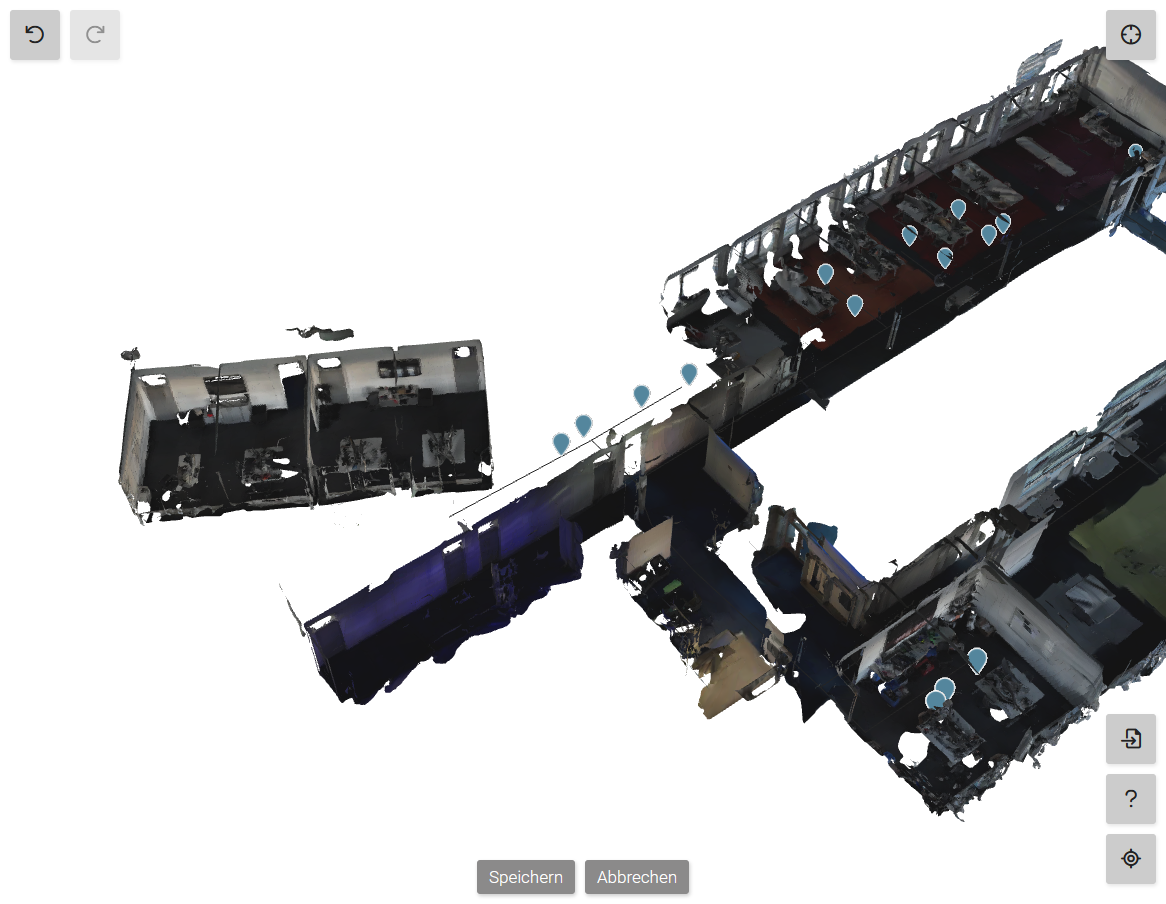
\includegraphics[width=0.9\textwidth]{Screenshot Editiermodus.png}
    \\
    Quelle: Eigene Darstellung
\end{figure}

Da der Boden bei allen 3D-Modellen ungefähr auf derselben z-Koordinate positioniert ist, müssen diese durch den Nutzer nicht weiter an der z-Achse verschoben werden. Im Vergleich zu den Roboterdaten sind die 3D-Modelle immer um 90° an der z-Achse und einen beliebigen Wert an der y-Achse rotiert, während die Rotation der x-Achse zwischen 3D-Modellen und Roboterdaten bereits übereinstimmt. Die 3D-Modelle werden im Editiermodus automatisch um -90° an der z-Achse rotiert und müssen vom Nutzer somit nur nach an der y-Achse rotiert werden. Die Roboterdaten und 3D-Modelle teilen sich bereits denselben Maßstab, weshalb der Nutzer nicht die Möglichkeit braucht die Modelle zu skalieren. Es gilt zu beachten, dass im Prototyp 3D-Modelle erwartet werden, die mit der Scaniverse App erzeugt wurden. In einem Produktivsystem sollten auch andere Quellen genutzt werden können. Die genannten Annahmen, dass die Modelle nicht um die z-Koordinate verschoben, nicht um die x- und z-Achse rotiert und nicht skaliert werden müssen, gelten dann nicht mehr. Somit bräuchte der Nutzer in einem Produktivsystem die Möglichkeit Modelle an allen Achsen zu verschieben und um alle Achsen zu rotieren. Auch müsste der Nutzer die Modelle skalieren können.

\subsection{Softwaretests}
Für eine größtmögliche Testabdeckung des entwickelten Prototyps wurden Unit und Integration Tests geschrieben. Das Testen der \deckgl{} Ansicht und Ebenen konnte nicht umgesetzt werden. So gibt es zwar den SnapshotTestRunner \cite{DeckglSnapshotTestRunner} mit dem das Framework testbar ist, dieser ist aber unzureichend dokumentiert, sodass die Tests nicht erfogreich implementiert werden konnten. Da die \deckgl{} Ansicht das Herzstück des Prototyps ist, ist die Testabdeckung unzureichend, aber unglücklicherweise auch nicht ausbaubar. Damit die Testabdeckung ausreicht muss erzwungenermaßen davon ausgegangen werden, dass die \deckgl{} Elemente ohne Fehler implementiert wurden. Es wurden Unit Tests für verschiedene Utility-Funktionen, für die komplexeren Redux Selektoren und für weitere Funktionen geschrieben. Die Redux Implementierung wurde bewusst nicht direkt getestet da es sich hierbei um Implementierungsdetails handelt die nach Kent C. Dodds nicht getestet werden sollten \cite{Dodds}. Stattdessen wird die Redux Implementierung zusammen mit den Buttons und dem Routenplanungs-Popup über Integration Tests getestet. Diese Vorgehensweise wird auch vom Redux Maintainer Mark Erikson empfohlen \cite{Erikson}. Die Unit und Integration Tests sind in die im Folgenden erklärte Deployment-Pipeline integriert.

\subsection{Deployment}
Für das Veröffentlichen des Prototyps wird GitHub Actions in Kombination mit GitHub Pages genutzt. Mit GitHub Actions lässt sich die Build-, Test- und Deployment-Pipeline eines Projekts automatisieren \cite{GitHubActions}. Bei GitHub Pages handelt es sich um einen Hosting-Dienst, der in GitHub integriert ist und aus Repositories statische Websites erstellen kann \cite{GitHubPages}. So wird mithilfe der actions-gh-pages Github Action \cite{ActionsGhPages} bei der Aktualisierung des Haupt-Branches automatisch ein Build erstellt. Das GitHub Repository ist so konfiguriert, dass der erstellte Build automatisch mit GitHub Pages veröffentlicht wird.

Die Anwendung verwendet verschiedene Funktionen der chayns-api \cite{ChaynsApi}, wie beispielsweise das Anfordern eines Zugangstokens, ohne den Funktionen des Backends nicht aufgerufen werden können. Diese Funktionen sind nur innerhalb der chayns Umgebung nutzbar, weshalb die Anwendung nur funktioniert, wenn sie – wie in der Dokumentation des create-chayns-app Befehls beschrieben \cite{CreateChaynsApp} – als Custom Page auf einer chayns Seite eingebunden ist. Der Zugriff auf die meisten Endpunkte des \ac{BCB}s ist so eingeschränkt, dass diese nur von unternehmensinternen chayns Seiten aus aufgerufen werden können. Auf anderen chayns Seiten können die Steuerungs- und Verwaltungsfunktionen deshalb nicht oder nur eingeschränkt genutzt werden.

\newpage
\section{Evaluierung des Prototyps}
Im Folgenden wird gezeigt welche funktionalen Anforderungen erfüllt werden. Auch wird ausgewertet inwieweit die nicht funktionalen Anforderungen an die Usability und Performance erfüllt werden.

\subsection{Funktionale Anforderungen}
Im Abschnitt \ref{sec:FunctionalRequirements} werden die funktionalen Anforderungen erläutert. Die meisten dieser Anforderungen werden erfüllt, weshalb hier nur die nicht erfüllten Anforderungen erwähnt werden. Bei dem Protyp handelt es sich zwar - wie in den Anforderungen definiert - um eine responsive Webanwendung, sie funktioniert allerdings nicht auf allen Geräten vollständig. So können die für die Gebäudemodelle genutzten \ac{glTF}-Modelle nicht im Safari-Browser angezeigt werden, weil die Modelle das \ac{WebP} Bildformat für die Texturen nutzen und dieses noch nicht vollständig von Safari unterstützt wird \cite{CanIUseWebP}. Da es sich hierbei um eine Beschränkung des Safari-Browsers handelt, die in Zukunft von Apple behoben werden sollte und weil alle anderen Funktionen des Prototyps auch im Safari-Browser funktionieren, wurde hierfür kein Workaround entwickelt. Während die Positionsänderungen der Roboter animiert werden, ist das bei den Rotationsänderungen aufgrund eines Bugs in \deckgl{} nicht der Fall. Aus diesem Grund ist die Anforderung, dass der Roboter in der Übersicht fährt nur teilweise erfüllt.

Die Anforderungen an die Methode zur Gebäudemodell-Generierung konnten mit dem Einsatz des \ac{LiDAR}-Scannens weitestgehend erfüllt werden. Für die Methode wird ein neueres iPhone benötigt, welches man als Nutzer unter umständen bereits besitzt. Das Generieren der Modelle erfordert vergleichsweise wenig Aufwand, wobei dieser davon abhängig ist, wie gründlich das Scannen durchgeführt wird. Insgesamt ist für das Scannen nur wenig Know-How nötig, da es in der Scanniverse App gut und einfach erklärt wird. Die entstandenen Modelle müssen für den Prototyp manuell komprimiert werden, wofür beispielsweise das im Abschnitt \ref{sec:ModelFileFormat} erwähnte Webtool infrage kommt. In einem Produktivsystem könnten die Modelle aber auch mithilfe des \ac{glTF}-Transform \ac{npm}-Pakets \cite{glTF-Transform} automatisch beim Import in den Editiermodus komprimiert werden. Die Qualität der erzeugten Modelle variiert zum einen dadurch wie gründlich die Scans durchgeführt wurden und zum anderen dadurch welche Methode zur Komprimierung des Modells genutzt wird. Insbesondere kleinere Ungenaugkeiten in den erzeugten Modellen können ignoriert werden, solange diese keinen Einfluss auf die Übersichtlichkeit des Modells haben.

\subsection{Benutzerfreundlichkeit}
Die Benutzerfreundlichkeit wird sowohl anhand der Erfüllung der Usability Entscheidungsregeln als auch durch die Auswertung von Usability Tests beurteilt.

\subsubsection{Usability Heuristics}\label{sec:UsabilityHeuristics}
Die Usability Entscheidungsregeln konnten weitestgehend eingehalten werden. Im Folgenden wird aufgezeigt wie ein paar Entscheidungsregeln konkret eingehalten werden.

Die erste Regel besagt, dass der Nutzer immer innerhalb einer angemssenen Zeispanne durch geeignete Rückmeldungen mitbekommen sollte, was gerade passiert \cite[Regel 1]{Nielsen.1994}. Diese Regel ist durch verschiedene Features in der Übersicht und Steuerung erfüllt. Zum einen gibt es die Echtzeit-Aktualisierungen des Roboterstandorts und -status über die \gls{Websocket}-Verbindung mit dem \ac{BCB}. Zum anderen werden Statusänderungen auch über die Farben der Buttons signalisiert. Auch gibt es einen Wait Cursor, um Ladevorgänge anzuzeigen.

% Die zweite Regel erwartet, dass der Nutzer die Sprache der Anwendung versteht und somit beispielsweise möglichst wenig Fachsprache verwendet wird. In der Steuerung und Verwaltung gibt es nur wenig Text, da vor allem Icons eigesetzt werden. In der Verwaltungsansicht werden möglicherweise unklare Begriffe wie Ladestation über Tooltips erklärt. Außerdem werden Einstellungsänderungen über Dialoge erklärt.

Da Benutzer oft versehentlich Aktionen ausführen, gibt es die dritte Regel, die klar gekennzeichnete Abbruchoptionen fordert, damit unerwünschte Aktionen abgebrochen oder rückgängig gemacht werden können \cite[Regel 3]{Nielsen.1994}. Um die Kamera wieder in die Ausgangsposition zu bringen, wenn diese versehentlich an eine ungewünschte Position bewegt wurde, gibt es in der Übersicht einen entsprechenden Button. In der Steuerung gibt es außerdem einen Button mit dem der aktuelle Lieferauftrag des Roboters abgebrochen werden kann. Auch gibt es sowohl in der Steuerung als auch in der Verwaltung Bestätigungsdialoge mit denen neue Aktionen und Einstellungsänderungen bestätigt werden müssen. Im Editiermodus gibt es die Möglichkeit das Verschieben und Rotieren von Objekten rückgängig zu machen oder zu wiederholen. Auch gibt es im Editiermodus einen Button mit dem das Editieren ohne Speichern abgebrochen werden kann. In Abbildung \ref{fig:DialogScreenshot} wird der Bestätigungsdialog gezeigt, der beim Abbrechen der Roboter Aktionen geöffnet wird.

\begin{figure}[H]
    \caption{Bestätigungsdialog}\label{fig:DialogScreenshot}
    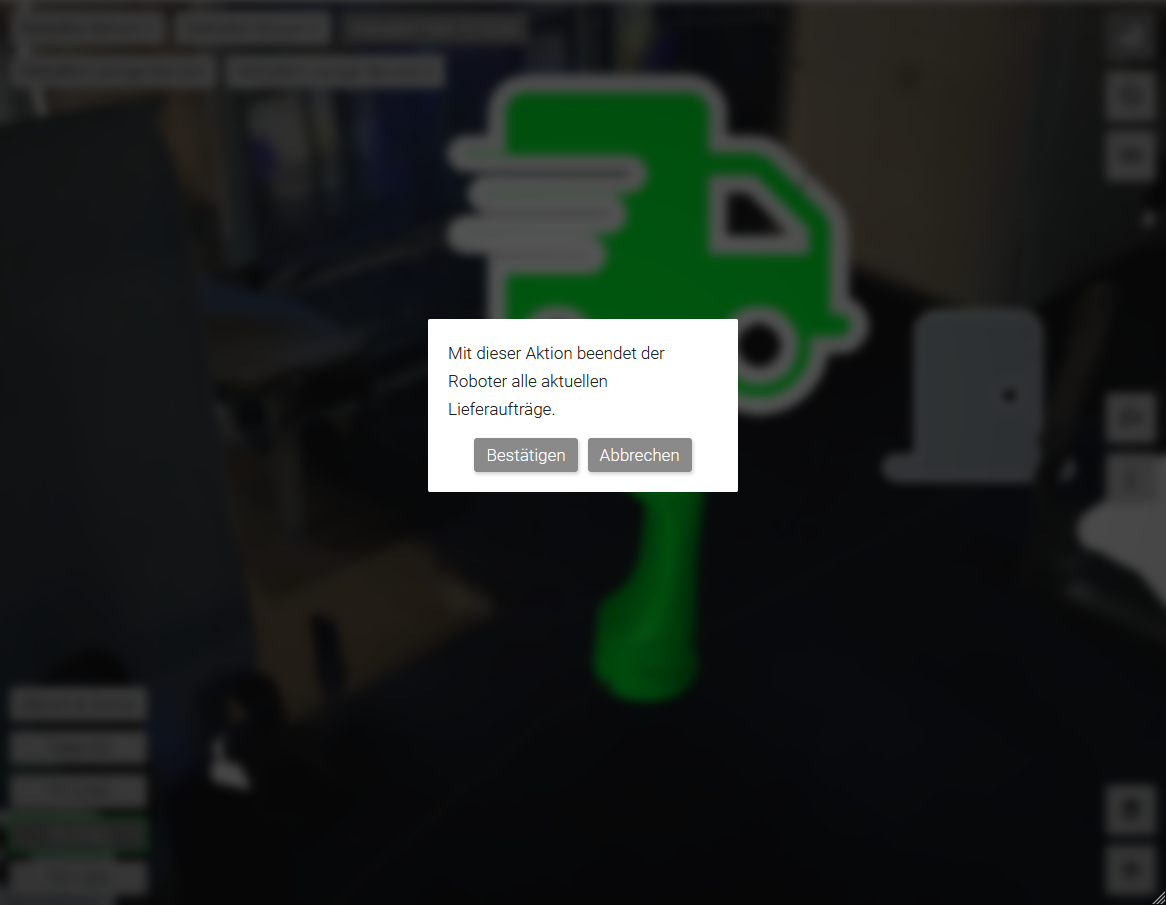
\includegraphics[width=0.9\textwidth]{Screenshot Dialog.png}
    \\
    Quelle: Eigene Darstellung
\end{figure}

In der fünften Regel geht es darum, dass Probleme, die Fehler auslösen, verhindert werden sollten \cite[Regel 5]{Nielsen.1994}. In der Steuerung ist es zum Beispiel nicht möglich ungültige Standorte in der Routenplanung einzugeben. Währenddessen wird diese Regel in der Verwaltung durch die bereits erwähnten Bestätigungsdialoge erfüllt. Im Editiermodus gibt es währenddessen die bereits erwähnte Rückgängigmachen und Wiederhohlen Funktion.

In der siebten Regel geht darum, dass bestimmte, häufig genutzte Aktionen mit Shortcuts schneller ausführbar sein sollten \cite[Regel 7]{Nielsen.1994}. So können Lieferstandort und Roboter für einen Lieferauftrag in der Steuerung sowohl über die Inputs als auch über die Karte ausgewählt werden. Im Editiermodus gibt es außerdem Tastenkombinationen für das Rückgängigmachen und Wiederhohlen.

Auch die anderen Usability Entscheidungsregeln wurden während der Entwicklung beachtet und weitestgehend erfüllt, was aber nicht automatisch bedeutet, dass der Prototyp auch wirklich benutzerfreundlich ist. Um das zu bestimmen folgen die Usability Tests.

\subsubsection{Usability Tests}\label{sec:UsabilityTests}
Während eines Großteils der Implementierung wurde die Benutzerfreundlichkeit nur oberflächlich durch den Entwickler bewertet, wodurch viel Zeit gespart wurde. Da sich die Entwickler von Systemen nicht zum Testen dieser eignen, konnten viele Probleme allerdings nicht identifiziert werden. Aus diesem Grund wurden Usability Tests mit ausgewählten Testpersonen durchgeführt, nachdem alle Funktionen des Prototyps erfolgreich implementiert wurden. Da die Benutzerfreundlichkeit des fertigen Prototyps bewertet werden soll und ein Vergleich zu vorherigen Versionen unwichtig ist, wurden qualitative statt quantitative Usability Tests durchgeführt.

Der Aufbau der Usability Tests basiert maßgeblich auf verschiedenen Artikeln der Nielsen Norman Group. So wurden die Aufgaben nach dem Stepped-User-Tasks-System \cite{Pernice.2020} formuliert und während der Durchführung der Tests wurde darauf geachtet, dass die Testpersonen die Thinking-Aloud-Methode \cite{Nielsen.2012b} einsetzen. Die ausführlicheren Tests wurden in zwei Runden mit jeweils fünf Personen durchgeführt. So konnten die gefundenen Probleme nach der ersten Runde behoben werden, bevor die zweite Runde durchgeführt wurde. Für die Usability Tests wurden drei Aktivitäten vorbereitet, die die Testpersonen nacheinander durchführen sollten. Die Aktivitäten decken direkt oder indirekt einen großen Teil der Funktionen des Prototyps ab. Konkret beschäftigen sich die Aktivitäten mit der Übersicht, der Steuerung und dem Editiermodus. In der ersten Aktivität müssen Position und Akkustand eines bestimmten Roboters gefunden werden. Daraufhin muss der Roboter in der zweiten Aktivität zu einem oder mehreren Standorten und dann zurück zur Ladestation geschickt werden. In der dritten Aktivität muss ein 3D-Modell mithilfe des Editiermodus richtig positioniert werden. In der dritten Aktivtiät wird beispielsweise nicht nur geprüft wie Benutzerfreundlich das Editieren ist, sondern auch wie leicht der Editiermodus überhaupt gefunden werden kann.

Um die geplanten Aktivitäten zu prüfen wurde zunächst ein Pilottest durchgeführt. Mithilfe von Pilottests können Probleme im Design von Tests gefunden werden, sodass diese vor der Durchführung der richtigen Tests aus dem Weg geschafft werden können \cite{Schade.2015}. Mithilfe des Pilottests konnten die Aktivitäten optimiert werden. Außerdem konnten die Ergebnisse des Pilottests bezüglich der Benutzerfreundlichkeit des Prototyps ausgewertet werden, sodass viele Probleme behoben werden konnten, bevor die anderen Tests durchgeführt wurden.

\paragraph{Erste Usability Test Runde}

In den beiden folgenden Tabellen werden die Ergebnisse des ersten Usability Testdurchlaufs zusammengefasst. Der Pilottest wird zu dieser Runde dazugezählt und ist in den Tabellen als T0 gekennzeichnet. In Tabelle \ref{tbl:1stUsabilityTestsProblems} wird dargestellt, welche Probleme bei welcher Testperson aufgefallen sind. So sieht man, dass die meisten Probleme die im Pilottest aufgefallen sind, danach nicht mehr aufgetreten sind, was darauf zurückzuführen ist, dass diese vor der Durchführung der restlichen Tests behoben wurden. Man kann zudem sehen, dass den meisten Testpersonen mindestens ein Problem aufgefallen ist, das keiner anderen Testperson aufgefallen ist. Hierdurch zeigt sich, dass durch weniger Testpersonen weniger Probleme gefunden worden wären. In Tabelle \ref{tbl:1stUsabilityTestsProblemsDesc} im Anhang werden die gefundenen Probleme genauer beschrieben. Bei der Korrektur der Probleme wurden die Probleme priorisiert, die besonders vielen Testpersonen aufgefallen sind. Durch die Usability Tests gab es außerdem zusätzlich Feedback der Testpersonen, das in der folgenden Implementierungsphase berücksichtigt wurde.

\begin{table}[H]
    \caption{Gefundene Probleme in erster Usability Test Runde}\label{tbl:1stUsabilityTestsProblems}
    \begin{tabular}{l||l|l|l|l|l|l}
                & T0    & T1    & T2    & T3    & T4    & T5    \\ \hline
    Problem 1   & X     &       &       & X     &       &       \\
    Problem 2   & X     &       &       &       &       &       \\
    Problem 3   & X     &       &       &       &       &       \\
    Problem 4   & X     &       &       &       &       &       \\
    Problem 5   & X     &       &       &       &       &       \\
    Problem 6   & X     &       & X     &       &       &       \\
    Problem 7   & X     &       &       &       &       &       \\
    Problem 8   & X     &       &       &       & X     &       \\
    Problem 9   &       & X     &       &       &       &       \\
    Problem 10  &       & X     &       &       &       &       \\
    Problem 11  &       & X     & X     & X     & X     &       \\
    Problem 12  & X     & X     & X     &       &       &       \\
    Problem 13  &       &       & X     &       &       &       \\
    Problem 14  &       &       & X     & X     &       &       \\
    Problem 15  & X     &       & X     &       &       &       \\
    Problem 16  &       &       &       & X     &       &       \\
    Problem 17  &       &       &       & X     &       &       \\
    Problem 18  &       &       &       &       &       & X     \\
    Problem 19  &       &       &       &       &       & X     \\
    Problem 20  &       &       &       &       &       & X     \\
    \end{tabular}    
\end{table}

In Tabelle \ref{tbl:1stUsabilityTestsActions} sind die Aktivitäten in verschiedene Aktionen aufgeteilt, die bei der Ausführung der Aktivität durchgeführt werden können, aber nicht unbedingt durchgeführt werden müssen. Die Werte zeigen, wie gut eine Aktion von einer Testperson durchgeführt werden konnte. Je niedriger der Wert, desto weniger Probleme sind aufgetreten. Kein Wert bedeutet, dass die Testperson die Aktion nicht durchgeführt hat, da die Aktion für den Erfolg der Aktivität nicht benötigt wurde. Somit wird die Benutzerfreundlichkeit in den entsprechenden Teilen der Anwendung ersichtlich. Man sieht, dass die meisten Aktionen nach dem Pilottest deutlich besser durchgeführt werden konnten, was auf die erwähnten Anpassungen am Prototyp zurückzuführen ist. Die Tabelle \ref{tbl:1stUsabilityTestsActions} zeigt, dass die meisten Aktionen zuverlässig durchgeführt werden können, sie zeigt aber auch, dass die Benutzerfreundlichkeit an einigen Stellen noch ausbaufähig ist. Insbesondere der Editiermodus hat Mängel, aber auch in der Übersicht und Steuerung gibt es kleinere Probleme.


\begin{table}[H]
    \caption{Bewertung der durchgeführten Aktionen in erster Usability Test Runde}\label{tbl:1stUsabilityTestsActions}
    \begin{tabular}{l||llllll}
        Aktion                              & T0        & T1        & T2        & T3        & T4        & T5        \\ \hline
        \textbf{Aktivität 1 (Übersicht)}    &           &           &           &           &           &           \\
        Roboter mit Button ausgewählt       &         1 &         1 &         1 &         1 &         1 &         1 \\
        Akkustand gefunden                  &         2 &         1 &         1 &         2 &         2 &         1 \\
        Roboter mit Folgen-Button gefunden  &         2 &         1 &         1 &         - &         - &         - \\
        Roboter mit Karte gefunden          &         - &         - &         - &         2 &         1 &         1 \\ \hline

        \textbf{Aktivtiät 2 (Steuerung)}    &           &           &           &           &           &           \\
        Lieferauftrag-Button gefunden       &         1 &         1 &         1 &         1 &         1 &         1 \\
%       Roboter mit Karte ausgewäht         &         - &         - &         - &         - &         - &         1 \\
        Standort mit Personfinder ausgewählt&         2 &         - &         1 &         1 &         1 &         1 \\
        Standort mit Karte ausgewählt       &         - &         1 &         - &         - &         1 &         1 \\
        Lieferauftrag gestartet             &         3 &         2 &         1 &         1 &         1 &         1 \\
        Roboter zur Ladestation geschickt   &         - &         1 &         1 &         1 &         1 &         1 \\ \hline

        \textbf{Aktivität 3 (Editiermodus)} &           &           &           &           &           &           \\
        Editormodus über Adminansicht       &         3 &         - &         - &         - &         - &         - \\
        Editormodus über Nutzeransicht      &         - &         1 &         1 &         1 &         1 &         1 \\
        Steuerung verstanden                &         - &         1 &         3 &         1 &         2 &         1 \\
        Undo/Redo genutzt                   &         - &         - &         - &         - &         - &         - \\
        Modell positioniert                 &         2 &         1 &         2 &         1 &         1 &         1 \\
    \end{tabular}
\end{table}


\paragraph{Zweite Usability Tests Runde}

Die Ergebnisse der ersten Usability Tests Runde wurden in der darauffolgenden Implementierungsphase einbezogen. Verschiedene Probleme wurden behoben und Feedback wurde umgesetzt. Daraufhin wurde eine neue Runde an Usability Tests mit fünf neuen Testpersonen durchgeführt. Die Ergebnisse sind in den folgenden zwei Tabellen abgebildet. Die Tabellen folgen der Struktur der vorherigen Tabellen. So zeigt Tabelle \ref{tbl:2ndUsabilityTestsProblems}, welche Testperson welche Probleme hatte und Tabelle \ref{tbl:2ndUsabilityTestsActions} wie gut Aktionen durchgeführt werden konnten. In Tabelle \ref{tbl:2ndUsabilityTestsProblemsDesc} im Anhang werden die gefundenen Probleme beschrieben. 

Man sieht in Tabelle \ref{tbl:2ndUsabilityTestsProblems}, dass deutlich weniger Probleme aufgefallen sind. Neben den Problemen gab es auch noch weiteres Feedback, dass sich aber vor allem auf Rechtschreibung, Zeichensetzung und Benennung beschränkt. Außerdem ist aus dem Feedback erkenntlich, dass das erste Auffinden von bestimmten Funktion etwas dauern kann, die Bedienung dieser Funktionen dann aber einwandfrei funktioniert. Es ist zu erwarten, dass die Bedienung des Prototyps bei einer erneuten Nutzung deutlich leichter ist, da die Funktionen dann nicht mehr lange gesucht werden müssen.

\begin{table}[H]
    \caption{Gefundene Probleme in zweiter Usability Test Runde}\label{tbl:2ndUsabilityTestsProblems}
    \begin{tabular}{l||l|l|l|l|l|l}
                    & T1    & T2    & T3    & T4    & T5    \\ \hline
        % Beim entfernen der Roboter Auswahl wird fälschlicherweise in das Stockwerk des Roboters gewechselt bei dem die Auswahl entfernt wurde
        Problem 1   & X     &       &       &       &       \\
        % Steuerungsbuttons müssen nicht immer aktiv sein (Abbrechen, wenn kein Lieferauftrag existiert; Laden, wenn bereits geladen wird)
        Problem 2   & X     &       &       &       &       \\
        % Roboter kann nicht über die Karte (ohne den "zur Ladestation" Button) zur Ladestation geschickt werden
        Problem 3   &       & X     &       &       &       \\
        % Suchfunktion von Standorten wurde nicht gefunden, weil diese im Lieferauftrag versteckt ist
        Problem 4   &       &       & X     &       &       \\
        % Irritation, dass Erklärung der Steuerung im Tooltip steht und nicht einfach permanent angezeigt an einer anderen Position angezeigt wird
        Problem 5   &       &       &       & X     &       \\
        % Editiermodus im Adminmodus nicht gefunden
        Problem 6   &       &       &       &       & X     \\
        % Editiermodus im Nutzermodus nicht gefunden
        Problem 7   &       &       &       &       & X     \\
    \end{tabular}    
\end{table}

Auch in Tabelle \ref{tbl:2ndUsabilityTestsActions} fällt auf, dass deutlich weniger Probleme aufgetreten sind. So gab es nur bei der zweiten und fünften Testperson geringfügige bis erhebliche Probleme. Bei der zweiten Testperson wurde erst versucht den Roboter direkt über eine Auswahl auf der Karte zur Ladestation zu schicken, während die fünfte Testperson Probleme damit hatte den Editiermodus zu finden, wobei hierfür ohne Erfolg in der Verwaltung gesucht wurde, bevor der Editiermodus in der Nutzeransicht gefunden wurde. So handelt es sich hier um Probleme die bei einer erneuten Nutzung der Anwendung nicht mehr auftreten würden. Nachdem die Tests ausgewertet wurden, wurde der Prototyp erneut angepasst, wodurch die beiden genannten Probleme nicht mehr auftreten sollten. Auch die in Tabelle \ref{tbl:2ndUsabilityTestsProblems} aufgelisteten Probleme wurden behoben.

\begin{table}[H]
    \caption{Bewertung der durchgeführten Aktionen in zweiter Usability Test Runde}\label{tbl:2ndUsabilityTestsActions}
    \begin{tabular}{l||llllll}
        Aktion                              & T1    & T2    & T3    & T4    & T5    \\ \hline
        \textbf{Aktivität 1 (Übersicht)}    &       &       &       &       &       \\
        Roboter mit Button ausgewählt       & 1     & 1     & 1     & 1     & 1     \\
        Akkustand gefunden                  & 1     & 1     & 1     & 1     & 1     \\
        Roboter mit Folgen-Button gefunden  & -     & -     & -     & -     & -     \\
        Roboter mit Karte gefunden          & 1     & 1     & 1     & 1     & 1     \\ \hline
        \textbf{Aktivtiät - (Steuerung)}    &       &       &       &       &       \\
        Lieferauftrag-Button gefunden       & 1     & -     & -     & -     & 1     \\
%       Roboter mit Karte ausgewäht         & -     & -     & -     & -     & -     \\
        Standort mit Personfinder ausgewählt& 1     & -     & -     & -     & 1     \\
        Standort mit Karte ausgewählt       & -     & 1     & 1     & 1     & -     \\
        Lieferauftrag gestartet             & 1     & 1     & 1     & 1     & 1     \\
        Roboter zur Ladestation geschickt   & 1     & 2     & 1     & 1     & 1     \\ \hline
        \textbf{Aktivität 3 (Editiermodus)} &       &       &       &       &       \\
        Editormodus über Adminansicht       & -     & -     & -     & -     & 3     \\
        Editormodus über Nutzeransicht      & 1     & 1     & 1     & 1     & 2     \\
        Steuerung verstanden                & 1     & 1     & 1     & 1     & 1     \\
        Undo/Redo genutzt                   & -     & -     & 1     & -     & 1     \\
        Modell positioniert                 & 1     & 1     & 1     & 1     & 1     \\
    \end{tabular}
\end{table}

Da die Menge der gefundenen Probleme mit dem zweiten Durchlauf der Tests stark abgenommen hat und da die Aktivitäten fast ohne Probleme durchgeführt wurden, wurde auf einen dritten Durchlauf verzichtet. Es ist nicht zu erwarten, dass ein dritter Durchlauf bedeutende neue Erkentnisse liefern würde, da aufgrund der Ergebnisse der vorherigen Tests angenommen werden kann, dass nur noch wenige Probleme bestehen, die auch mit einem erneuten Durchlauf nicht unbedingt gefunden werden können. Es ist wichtig zu beachten, dass mit den Usability Tests nicht alle Funktionen des Prototyps getestet wurden. Stattdessen wurden nur die wichtigsten Funktionen getestet die mit \deckgl{} in Verbindung stehen und somit für die Forschungsfrage dieser Arbeit größere Relevanz haben. Ob die Liste der Roboter und Stockwerke in der Verwaltung besonders Benutzerfreundlich ist, ist für die Forschungsfrage nicht besonders relevant, da diese Liste sehr simpel ist und keine besonderen Technologien nutzt. In Kombination mit der Einhaltung der Usability Entscheidungsregeln ist davon auszugehen, dass das Ziel der Benutzerfreundlichkeit ausreichend erfüllt wurde.

\subsection{Performance}
% TODO An Anforderungen Kapitel orientieren!
Wie im Abschnitt \ref{sec:PerformanceBasics} beschrieben werden \ac{PLS}, \ac{LR} und Smoothness gemessen. Für die Bestimmung des \ac{PLS} wird der \ac{FCP} gemessen. Normalerweise wird hierfür der \ac{LCP} gemessen. Allerdings kann die Ladezeit des wichtigsten Elements - der \deckgl{} Karte - nicht gemessen werden. Die \ac{LR} wird über den \ac{FID} und die \ac{TBT} gemessen. Die Smoothness wird nur öberflächig ohne Messwert überprüft.

TODO: Ergebnisse erläutern.

% Metriken kurz erklären
% First Contentful Paint
% Largest Contentfult Paint => Nicht nutzbar, da das Rendern der deck.gl Layers nicht über Events erkannt werden kann
% First Input Delay
% Total Blocking Time
% Erläutern warum die Richtwerte nicht erreicht werden können, die Performance aber trotzdem in Ordnung ist



% => Performance Tests (testen welche Maßnahmen welche Performance Auswirkungen haben)
% Maßnahmen
% Nutzung des .glb Formats statt .obj (beides mit und ohne Kompression)
    % Einfluss auf Ladezeiten (Netzwerk und Rendering)
    % Einfluss auf GPU und CPU Auslastung
% Caching der Robotermodelle
% Caching aller anderen Anfragen (Bis auf Roboter)
% Sehr Kurzzeitiges Caching der Roboter
% Initialisierung der Karten Vorschau über Button statt beim Öffnen des Aufklappers (vielleicht nicht ganz passend?)

\newpage
\section{Fazit}
Im Rahmen der Arbeit wurde die Forschungsfrage, wie eine effiziente und benutzerfreundliche Steuerung und Verwaltung von Servicerobotern implementiert werden kann beantwortet. Hierfür wurde erfolgreich ein Prototyp implementiert, der iterativ entwickelt und auf die verschiedenen Anforderungen geprüft wurde. Die aus der Zielsetzung, Forschungsfrage und Umgebung herausgearbeiteten Anforderungen wurden weitestgehend erfüllt. So handelt es sich bei dem Prototyp um eine benutzerfreundliche und effiziente Webanwendung.

\subsection{Nutzung des Prototyps}
Der lauffähige Prototyp ist mithilfe der Anleitung – die sich in der Datei Prototyp.txt in den Zusatzdokumenten befindet – erreichbar und nutzbar. Es gilt zu beachten, dass die meisten Verwaltungs- und Steuerungsfunktionen aus Sicherheitsgründen nicht genutzt werden können. Um welche Funktionen es sich genau handelt, ist in der Anleitung beschrieben.

%\subsection{Aufgetretene Probleme}
%Während der Entwicklung des Prototyps wurden verschiedene Probleme identifiziert, die mit \deckgl{} oder dem Einbinden von 3D-Modellen im Web in Verbindung stehen. So ist die SimpleMeshLayer des Frameworks dadurch beschränkt das \ac{OBJ} Dateien nur ohne die \mtl{} Datei, also ohne Textur eingebunden werden können. Dadurch musste bei der Anzeige der Gebäudemodelle auf die ScenegraphLayer zurückgegriffen werden und die Robotermodelle konnten nur einfarbig ohne Textur dargestellt werden. Insgesamt gibt es beim Animieren von 3D-Modellen verschiedene Probleme: In der ScenegraphLayer funktioniert das Animieren über die transition Property gar nicht, während in der SimpleMeshLayer nur das Animieren der Rotation nicht funktioniert. Da \deckgl{} \ac{WebGL} für die Darstellung nutzt, können automatisierte Tests nur über den Vergleich von Screenshots durchgeführt werden. Hierfür existiert zwar der SnapshotTestRunner der diesen Prozess automatisieren kann, die Klasse ist allerdings nicht ausreichend dokumentiert, weshalb \deckgl{} Funktionen im Prototyp nicht automatisch getestet werden können. Da das Framework ein Open-Source-Projekt ist und aktiv aktualisiert wird, können diese Probleme behoben werden, nachdem diese gemeldet wurden.

%Beim Einbinden von 3D-Modellen gibt es weitere Probleme, die unabhängig von \deckgl{} auftreten. So können die verwendeten \ac{glTF} Modelle mit \ac{WebP} Texturen nicht im Safari Browser genutzt werden. Auch gibt es an Mobilgeräten Probleme bei der Darstellung großer und somit rechenaufwändiger 3D-Modelle, was auf Hardwarebeschränkungen zurückzuführen ist.

\subsection{Ausblick}
Da die Anforderungen an den Prototyp erfüllt werden konnten ist der nächste logische Schritt die Implementierung als Produktivsystem. Wie bereits erwähnt, sind hierfür verschiedene Anpassungen im Prototyp und im \ac{BCB} nötig, die allerdings nicht sonderlich groß ausfallen. Im Backend müssen vor allem neue Endpunkte hinzugefügt und die Datenbank erweitert werden, damit die 3D-Modelle gespeichert, verändert und abgerufen werden können. Auch müssen die Standorte und Roboterpfade permanent im \ac{BCB} abgespeichert werden, damit nicht nur Daten von Stockwerken angefragt werden können, in denen sich Roboter befinden. Zusätzlich müssen die Produktqualitätsmerkmale untersucht werden, die im Rahmen dieser Arbeit vernachlässigt wurden. Hierbei handelt es sich um: Portabilität, Wartbarkeit, Sicherheit, Verlässlichkeit und Kompatibilität. Zuletzt sollte ein Produktivsystem auch den Import von 3D-Modellen aus anderen Quellen ermöglichen. Im gleichen Schritt könnte auch eine automatische Kompression der importierten Modelle implementiert werden.

Zusätzlich können auch weitere Aspekte erforscht werden, die im Rahmen dieser Arbeit nur oberflächlich betrachtet wurden. Wie bereits demonstriert wird kann \deckgl{} für mehr als nur für Geodatenvisualisierungen eingesetzt werden. So könnte genauer erforscht werden für welche weiteren Anwendungsszenarien sich das Framework noch eignet. Wie bereits erwähnt, sollen die Roboter auf ihre Zuverlässigkeit und Navigationsfähigkeit geprüft werden. Hierfür eignet sich eine wissenschaftliche Untersuchung anhand ausgewählter Kriterien. Zuletzt könnte noch untersucht werden, wie der konzipierte Editiermodus zum Verschieben und Rotieren auch für die Nutzung an Smartphones implementiert werden könnte. So ist der Editiermodus im Prototyp nur an Desktop Computern nutzbar, da die Steuerungs- und Umschalttasten benötigt werden.
% Forschungsfrage konnte beantwortet werden
% Modell Generierungsmethode ausreichend gut => kurz zeigen wo die LiDAR Gebäudescans Schwächen haben (Transparenz und Relektierende Objekte; bewegende Objekte => Gebäude muss leer sein, also nach Arbeitszeit)
% Prototyp ist benutzerfreundlich und zumindest ausreichend effizient (trotz Webanwendung und 3D-Darstellung)
% Gutes Feedback von Testpersonen; Zum Teil auch leichte Begeisterung über 3D-Darstellung
% Karten Handling sehr zielführend => Google Maps bereits vertraut
% deck.gl kann für mehr als für Geodatenvisualisierungen genutzt werden

% Zeigen wo die Steuerung erreichbar ist

% Verschiedene Probleme mit 3D-Darstellung in deck.gl
% deck.gl hat leider mehrere kleinere Bugs => Die aber wegen Open Source schnell gelöst werden können
% Unzureichende Dokumentation der Snapshot Tests in deck.gl => Geringe Code Coverage der Tests
% Auch Webbrowser noch nicht vollständig auf 3D-Darstellung ausgelegt => glTF mit WebP funktioniert nicht an Safari Geräten
% Mobilgeräte haben Probleme mit besonders großen 3D-Modellen

% Anpassungen für ein Potenzielles Produktivsystem zusammenfassen
% Vom Prototyp zum Produktivsystem fehlt nicht viel => verschiedene Backend und Datenbank Anpassungen; Anpassungen im Frontend (importierte 3D-Modelle im chayns.space abspeichern; erweiterte Routenplanung)
% Anpassungen wären nötig damit nicht nur 3D-Modelle aus Scaniverse App akzepziert werden können


% Ausblick
% Genauerer Vergleich zwischen LiDAR Scanning, Fotogrammetrie und KI
% Vergleich zwischen deckgl und three.js oder anderen Frameworks
% Falls ein Produktivsystem umgesetzt, dieses untersuchen => besonders auch auf den Einsatz bei Kellnern
% Eignung der Service Roboter untersuchen (Zuverlässigkeit, Navigationsfähigkeit)
% Editiermodus für Smartphones => verschieben und rotieren von 3D-Modellen über Touch



%-----------------------------------
% Apendix / Anhang
%-----------------------------------
\newpage
\section*{\AppendixName} %Überschrift "Anhang", ohne Nummerierung
\addcontentsline{toc}{section}{\AppendixName} %Den Anhang ohne Nummer zum Inhaltsverzeichnis hinzufügen

\begin{appendices}
% Nachfolgende Änderungen erfolgten aufgrund von Issue 163
\makeatletter
\renewcommand\@seccntformat[1]{\csname the#1\endcsname:\quad}
\makeatother
\addtocontents{toc}{\protect\setcounter{tocdepth}{0}} %
	\renewcommand{\thesection}{\AppendixName\ \arabic{section}}
	\renewcommand\thesubsection{\AppendixName\ \arabic{section}.\arabic{subsection}}
	\section{Bilder}
\begin{figure}[H]
    \centering
    \caption{Mockup der Übersicht}\label{fig:MockupOverview}
    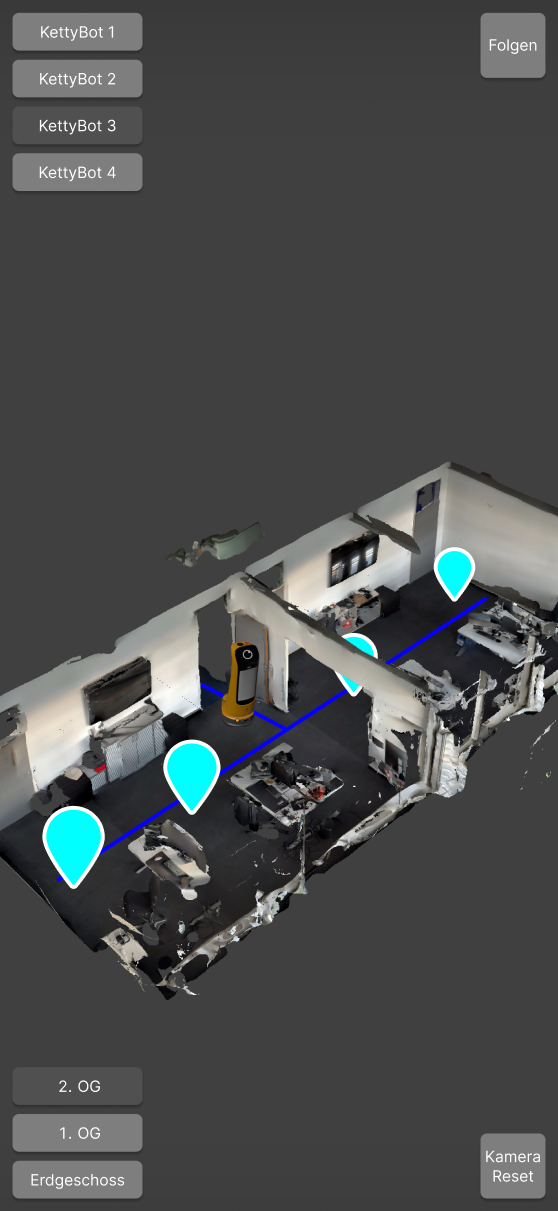
\includegraphics[width=0.5\textwidth]{Mockup Uebersicht}
    \\
    Quelle: Eigene Darstellung
\end{figure}

\begin{figure}[H]
    \centering
    \caption{Mockup der Steuerung}\label{fig:MockupControls}
    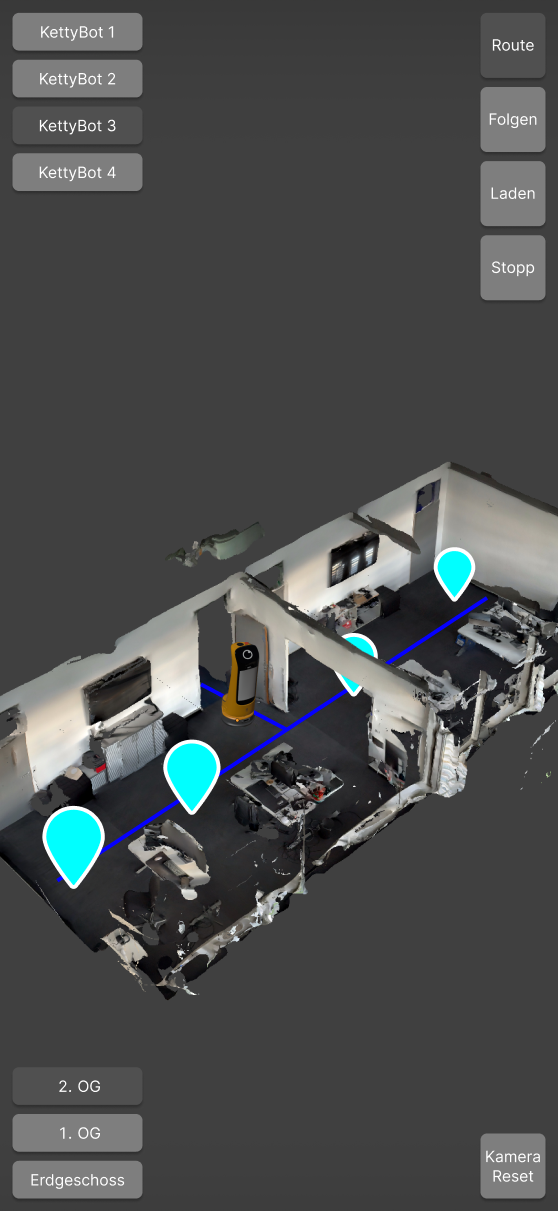
\includegraphics[width=0.5\textwidth]{Mockup Steuerung}
    \\
    Quelle: Eigene Darstellung
\end{figure}

\begin{figure}[H]
    \centering
    \caption{Mockup des Routenplanungs-Popup}\label{fig:MockupRoutePlanner}
    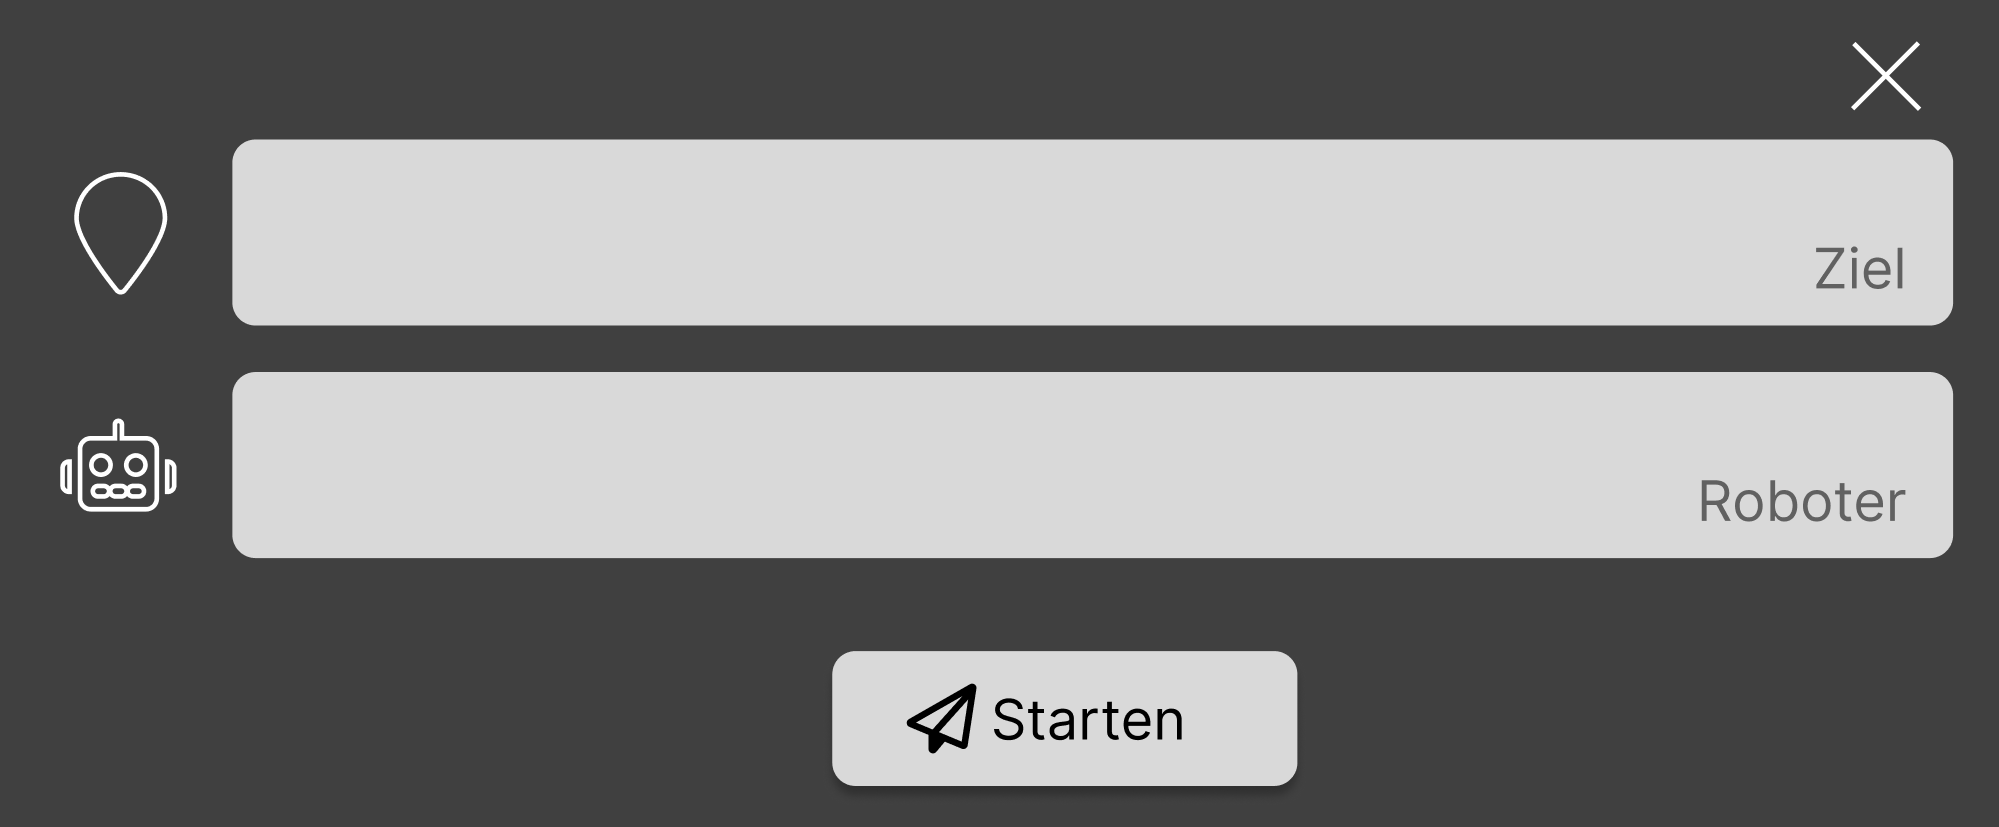
\includegraphics[width=0.9\textwidth]{Mockup Routenplaner}
    \\
    Quelle: Eigene Darstellung
\end{figure}

\begin{figure}[H]
    \centering
    \caption{Mockup der Verwaltung}\label{fig:MockupAdministration}
    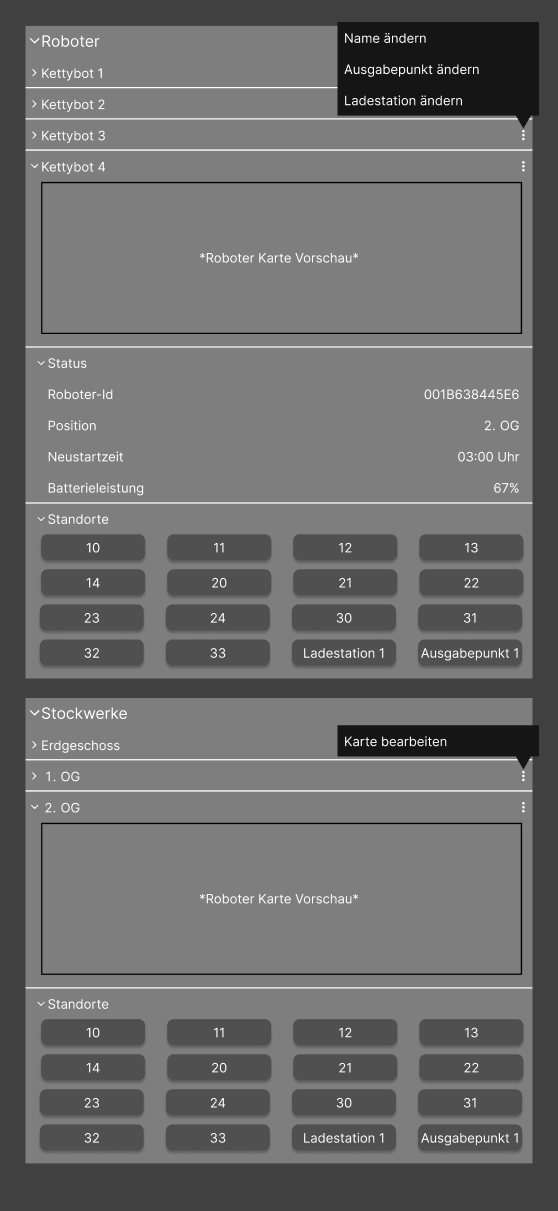
\includegraphics[width=0.5\textwidth]{Mockup Verwaltung}
    \\
    Quelle: Eigene Darstellung
\end{figure}

\section{Tabellen}
\begin{table}[H]
    \caption{Beschreibung der Probleme in erster Usability Testrunde}\label{tbl:1stUsabilityTestsProblemsDesc}
    \begin{tabular}{l|l}
        Problem     & Beschreibung \\ \hline
        Problem 1   & \multicolumn{1}{p{12cm}}{Der Ladestation Button mit Akkustand verwechselt.} \\ \hline
        Problem 2   & \multicolumn{1}{p{12cm}}{Die Icons der Buttons sind nicht selbsterklärend. Ohne anklicken der Buttons kennt man die Funktionen nicht.} \\ \hline
        Problem 3   & \multicolumn{1}{p{12cm}}{Die Anordnung der Ergebnisse im Input Dropdown suggeriert, dass man nur nach Nummern und nicht nach Namen suchen kann.} \\ \hline
        Problem 4   & \multicolumn{1}{p{12cm}}{Die Tooltips auf der Karte sind durch die Farben schlecht lesbar.} \\ \hline
        Problem 5   & \multicolumn{1}{p{12cm}}{Die Fehlermeldungen erklären das Problem nicht.} \\ \hline
        Problem 6   & \multicolumn{1}{p{12cm}}{Es wurde versucht die Modelle in der Übersicht zu verschieben, statt in den Editiermodus zu wechseln.} \\ \hline
        Problem 7   & \multicolumn{1}{p{12cm}}{Erklärung der Steuerung im Editiermodus ist nicht eindeutig genug.} \\ \hline
        Problem 8   & \multicolumn{1}{p{12cm}}{Ohne Loslassen der Maus kann nicht zwischen Verschieben und Rotieren des Modells gewechselt werden.} \\ \hline
        Problem 9   & \multicolumn{1}{p{12cm}}{Es wurde erwartet, dass man in der Routenplanung mehrere Ziele einstellen kann.} \\ \hline
        Problem 10  & \multicolumn{1}{p{12cm}}{Es wurde erwartet, dass die Ladestation in der Routenplanung eingestellt werden kann.} \\ \hline
        Problem 11  & \multicolumn{1}{p{12cm}}{Der Toast Dialog der die Steuerung im Editiermodus wurde nicht angezeigt.} \\ \hline
        Problem 12  & \multicolumn{1}{p{12cm}}{Unklarheit darüber wohin das 3D-Modell verschoben werden muss. Hierbei handelt es sich um ein Problem mit der Aktivität und nicht mit dem Prototyp.} \\ \hline
        Problem 13  & \multicolumn{1}{p{12cm}}{Darstellung der 3D-Modelle sieht kaputt aus.} \\ \hline
        Problem 14  & \multicolumn{1}{p{12cm}}{Ein Stockwerk-Button wird durch das Beta Modus Tag von chayns verdeckt.} \\ \hline
        Problem 15  & \multicolumn{1}{p{12cm}}{Es gab Schwierigkeiten beim Positionieren des Modells.} \\ \hline
        Problem 16  & \multicolumn{1}{p{12cm}}{Der Roboter wurde aufgrund des Icons – das über diesem angezeigt wird – nicht erkannt.} \\ \hline
        Problem 17  & \multicolumn{1}{p{12cm}}{Die Transparenz der Lieferauftrag-Fläche macht Text schlecht lesbar und sieht insgesamt nicht gut aus.} \\ \hline
        Problem 18  & \multicolumn{1}{p{12cm}}{Die Robotersteuerungs-Buttons werden nicht angezeigt, wenn die Routenplanung geöffnet ist.} \\ \hline
        Problem 19  & \multicolumn{1}{p{12cm}}{Es wurde erwartet, dass man nach dem Schließen des Eidtiermodus wieder im Nutzermodus landet.} \\ \hline
        Problem 20  & \multicolumn{1}{p{12cm}}{Der Button zum Zurücksetzen der Kameraposition wurde im Editiermodus nicht gefunden, da dieser an einer anderen Position als in der Übersicht angezeigt wird.} \\
    \end{tabular}
\end{table}
\begin{table}[H]
    \caption{Beschreibung der Probleme in zweiter Usability Testrunde}\label{tbl:2ndUsabilityTestsProblemsDesc}
    \begin{tabular}{l|l}
        Problem     & Beschreibung \\ \hline
        Problem 1   & \multicolumn{1}{p{12cm}}{Unklarheit darüber wie man die Karte rotiert.} \\ \hline
        Problem 2   & \multicolumn{1}{p{12cm}}{Beim Entfernen einer Roboterauswahl, wird in das Stockwerk des Roboters gewechselt, obwohl das nur bei der Auswahl eines Roboters passieren sollte.} \\ \hline
        Problem 3   & \multicolumn{1}{p{12cm}}{Es wurde erwartet, dass man den Roboter über das Ladestations-Icon auf der Karte zur Ladestation schicken kann.} \\ \hline
        Problem 4   & \multicolumn{1}{p{12cm}}{Suchfunktion zum Auswählen eines Standorts nicht gefunden, da das Routenplanungs-Popup nicht geöffnet wurde.} \\ \hline
        Problem 5   & \multicolumn{1}{p{12cm}}{Irritation darüber, dass die Steuerung über einen Tooltip erklärt wird.} \\ \hline
        Problem 6   & \multicolumn{1}{p{12cm}}{Editiermodus nicht im Nutzermodus gefunden, da das Icon des Buttons falsch verstanden wurde.} \\ \hline
        Problem 7   & \multicolumn{1}{p{12cm}}{Editiermodus nicht im Admin-Modus gefunden, da das Kontextmenü übersehen wurde.}
    \end{tabular}
\end{table}

\end{appendices}
\addtocontents{toc}{\protect\setcounter{tocdepth}{2}}

%-----------------------------------
% Literaturverzeichnis
%-----------------------------------
\newpage

% Die folgende Zeile trägt ALLE Werke aus literatur.bib in das
% Literaturverzeichnis ein, egal ob sie zietiert wurden oder nicht.
% Der Befehl ist also nur zum Test der Skripte sinnvoll und muss bei echten
% Arbeiten entfernt werden.
%\nocite{*}

%\addcontentsline{toc}{section}{Literatur}

% Die folgenden beiden Befehle würden ab dem Literaturverzeichnis wieder eine
% römische Seitennummerierung nutzen.
% Das ist nach dem Leitfaden nicht zu tun. Dort steht nur dass 'sämtliche
% Verzeichnisse VOR dem Textteil' römisch zu nummerieren sind. (vgl. S. 3)
%\pagenumbering{Roman} %Zähler wieder römisch ausgeben
%\setcounter{page}{4}  %Zähler manuell hochsetzen

% Ausgabe des Literaturverzeichnisses

% Keine Trennung der Werke im Literaturverzeichnis nach ihrer Art
% (Online/nicht-Online)
%\begin{RaggedRight}
%\printbibliography
%\end{RaggedRight}

% Alternative Darstellung, die laut Leitfaden genutzt werden sollte.
% Dazu die Zeilen auskommentieren und folgenden code verwenden:

%\defbibfilter{notonline}{
%	type=misc or
%	type=article or
%	type=incollection or
%	type=inproceedings or
%	type=book
%}
%\defbibfilter{online}{
%	type=online or
%	type=software
%}

% Literaturverzeichnis getrennt nach Nicht-Online-Werken und Online-Werken
% (Internetquellen).
% Die Option nottype=online nimmt alles, was kein Online-Werk ist.
% Die Option heading=bibintoc sorgt dafür, dass das Literaturverzeichnis im
% Inhaltsverzeichnis steht.
% Es ist übrigens auch möglich mehrere type- bzw. nottype-Optionen anzugeben, um
% noch weitere Arten von Zusammenfassungen eines Literaturverzeichnisse zu
% erzeugen.
% Beispiel: [type=book,type=article]
\printbibliography[heading=bibintoc,title={\langde{Literaturverzeichnis}\langen{Bibliography}}]

% neue Seite für Internetquellen-Verzeichnis
\newpage

% Laut Leitfaden 2018, S. 14, Fussnote 44 stehen die Internetquellen NICHT im
% Inhaltsverzeichnis, sondern gehören zum Literaturverzeichnis.
% Die Option heading=bibintoc würde die Internetquelle als eigenen Eintrag im
% Inhaltsverzeicnis anzeigen.
%\printbibliography[type=online,heading=bibintoc,title={\headingNameInternetSources}]
%\printbibliography[filter=online,heading=subbibliography,title={\headingNameInternetSources}]

\newpage
\pagenumbering{gobble} % Keine Seitenzahlen mehr

%-----------------------------------
% Ehrenwörtliche Erklärung
%-----------------------------------
\section*{%
	\langde{Ehrenwörtliche Erklärung}
	\langen{Declaration in lieu of oath}}
\langde{Hiermit versichere ich, dass die vorliegende Arbeit von mir selbstständig und ohne unerlaubte Hilfe angefertigt worden ist, insbesondere dass ich alle Stellen, die wörtlich oder annähernd wörtlich aus Veröffentlichungen entnommen sind, durch Zitate als solche gekennzeichnet habe. Ich versichere auch, dass die von mir eingereichte schriftliche Version mit der digitalen Version übereinstimmt. Weiterhin erkläre ich, dass die Arbeit in gleicher oder ähnlicher Form noch keiner Prüfungsbehörde/Prüfungsstelle vorgelegen hat. Ich erkläre mich damit \textcolor{red}{einverstanden/nicht einverstanden}, dass die Arbeit der Öffentlichkeit zugänglich gemacht wird. Ich erkläre mich damit einverstanden, dass die Digitalversion dieser Arbeit zwecks Plagiatsprüfung auf die Server externer Anbieter hochgeladen werden darf. Die Plagiatsprüfung stellt keine Zurverfügungstellung für die Öffentlichkeit dar.}
\langen{I hereby declare that I produced the submitted paper with no assistance from any other party and without the use of any unauthorized aids and, in particular, that I have marked as quotations all passages which are reproduced verbatim or near-verbatim from publications. Also, I declare that the submitted print version of this thesis is identical with its digital version. Further, I declare that this thesis has never been submitted before to any examination board in either its present form or in any other similar version. I herewith \textcolor{red}{agree/disagree} that this thesis may be published. I herewith consent that this thesis may be uploaded to the server of external contractors for the purpose of submitting it to the contractors’ plagiarism detection systems. Uploading this thesis for the purpose of submitting it to plagiarism detection systems is not a form of publication.}


\par\medskip
\par\medskip

\vspace{5cm}

\begin{table}[H]
	\centering
	\begin{tabular*}{\textwidth}{c @{\extracolsep{\fill}} ccccc}
		\myOrt, \the\day.\the\month.\the\year
		&
		% Hinterlege deine eingescannte Unterschrift im Verzeichnis /abbildungen und nenne sie unterschrift.png
		% Bilder mit transparentem Hintergrund können teils zu Problemen führen
		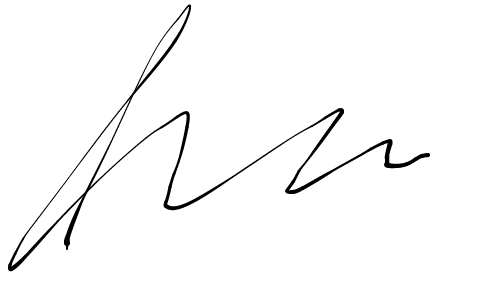
\includegraphics[width=0.35\textwidth]{unterschrift}\vspace*{-0.35cm}
		\\
		\rule[0.5ex]{12em}{0.55pt} & \rule[0.5ex]{12em}{0.55pt} \\
		\langde{(Ort, Datum)}\langen{(Location, Date)} & \langde{(Eigenhändige Unterschrift)}\langen{(handwritten signature)}
		\\
	\end{tabular*} \\
\end{table}

\end{document}
